% Paquets généraux
\documentclass[a4paper,12pt,titlepage,twoside]{article}
\usepackage[T1]{fontenc}
\usepackage[utf8]{inputenc}
\usepackage[french]{babel}
\addto\captionsfrench{%
  \renewcommand{\tablename}{Tableau}%
}
\usepackage[gen]{eurosym}
%\usepackage[dvips]{graphicx}
\usepackage{fancyhdr}
\usepackage{pdfpages} 
\usepackage{multido}
\usepackage{hyperref}
%\usepackage{textcomp}
\usepackage{schemabloc}
\usepackage[bitstream-charter]{mathdesign}
\usepackage{array}
\newcolumntype{P}[1]{>{\centering\arraybackslash}p{#1}}

\newcommand{\id}{54}
\newcommand{\nom}{Liaisons mécaniques}
\newcommand{\sequence}{04}
\newcommand{\num}{01}
\newcommand{\type}{TP}
\newcommand{\descrip}{Modélisation d'un solide. Comportement des liaisons mécaniques. Modéliser les mécanismes du laboratoire par un schéma cinématique, paramétré.}
\newcommand{\competences}{A3-C4: Analyse d'architecture et de comportement \\ &  Mod1-C1: Isolement d'un solide ou d'un système de solides \\ &  Mod2-C10-1: Modèle de solide indéformable \\ &  Mod2-C11: Modélisation géométrique et cinématique des mouvements entre solides indéformables \\ &  Mod2-C12: Modélisation cinématique des liaisons entre solides \\ &  Mod2-C15: Modélisation des actions mécaniques \\ &  Rés-C6: Utilisation d'un solveur ou d'un logiciel multi physique \\ &  Com1-C1: Différents descripteurs introduits dans le programme \\ &  Com2-C4: Outils de communication}
\newcommand{\nbcomp}{9}
\newcommand{\systemes}{Plateforme Stewart}
\newcommand{\systemessansaccent}{Plateforme Stewart}
\newcommand{\ilot}{2}
\newcommand{\ilotstr}{02}
\newcommand{\dossierilot}{\detokenize{Ilot_02 Plateforme Stewart}}
\newcommand{\imageun}{Plateforme}

\newcommand{\urlsysteme}{\href{https://www.costadoat.fr/systeme/57}{Ressources système}}
\newcommand{\matlabsimscape}{\href{https://github.com/Costadoat/Sciences-Ingenieur/raw/master/Systemes/Plateforme Stewart/Plateforme_Stewart_Simscape.zip}{Modèle Simscape}}
\newcommand{\solidworks}{\href{https://github.com/Costadoat/Sciences-Ingenieur/raw/master/Systemes/Plateforme Stewart/Plateforme_Stewart_Solidworks.zip}{Modèle Solidworks}}
\newcommand{\edrawings}{\href{https://github.com/Costadoat/Sciences-Ingenieur/raw/master/Systemes/Plateforme Stewart/Plateforme_Stewart.EASM}{Modèle eDrawings}}
\newcommand{\test}{Stewart_param1}
\newcommand{\testi}{Stewart_param2}
\newcommand{\testii}{Stewart_param3}
\newcommand{\testiii}{Stewart_param4}
\newcommand{\testiiii}{Stewart_euler}

\newcommand{\institute}{Lycée Dorian}

\usepackage{fancyvrb}
\usepackage{color}
\usepackage{xcolor}
\usepackage{colortbl}
\usepackage{helvet}
\renewcommand{\familydefault}{\sfdefault}
\usepackage{amsfonts}
\usepackage{amsmath}
%\usepackage{xspace}
\usepackage{varioref}
\usepackage{tabularx}
%\usepackage{floatflt}
\usepackage{graphics}
\usepackage{wrapfig}
\usepackage{textcomp}
\usepackage{tikz}
\usepackage{wrapfig}
\usepackage{gensymb}
\usepackage[percent]{overpic}
\usepackage[european]{circuitikz}
\usetikzlibrary{babel}
\usepackage{ifthen}
\usepackage{cancel}
\usepackage{etoolbox}
\usepackage{multirow}
%\usepackage{boxedminipage}
\definecolor{gris25}{gray}{0.75}
\definecolor{bleu}{RGB}{18,33,98}
\definecolor{bleuf}{RGB}{42,94,171}
\definecolor{bleuc}{RGB}{231,239,247}
\definecolor{rougef}{RGB}{185,18,27}
\definecolor{rougec}{RGB}{255,188,204}%255,230,231
\definecolor{vertf}{RGB}{103,126,82}
\definecolor{vertc}{RGB}{220,255,191}
\definecolor{forestgreen}{rgb}{0.13,0.54,0.13}
\definecolor{blcr}{rgb}{0.59,0.69,0.84}
\definecolor{blfr}{rgb}{0.32,0.51,0.75}
\definecolor{orfr}{rgb}{0.90,0.42,0.15}
\definecolor{orcr}{rgb}{0.90,0.65,0.50}
\definecolor{orangef}{rgb}{0.659,0.269,0.072}
\definecolor{orange}{rgb}{0.58,0.35,0.063}
\definecolor{orangec}{rgb}{0.43,0.32,0.25}
\definecolor{rcorrect}{rgb}{0.6,0,0}
\definecolor{sequence}{rgb}{0.75,0.75,0.75}
\definecolor{competences}{rgb}{0.61,0.73,0.35}
\definecolor{grisf}{HTML}{222222}
\definecolor{grisc}{HTML}{636363}
\definecolor{normal}{HTML}{4087c4}
\definecolor{info}{HTML}{5bc0de}
\definecolor{success}{RGB}{92,184,92}
\definecolor{warning}{RGB}{240,173,78}
\definecolor{danger}{RGB}{217,83,79}
\hypersetup{                    % parametrage des hyperliens
    colorlinks=true,                % colorise les liens
    breaklinks=true,                % permet les retours à la ligne pour les liens trop longs
    urlcolor= blfr,                 % couleur des hyperliens
    linkcolor= orange,                % couleur des liens internes aux documents (index, figures, tableaux, equations,...)
    citecolor= forestgreen                % couleur des liens vers les references bibliographiques
    }

% Mise en page
\pagestyle{fancy}

\setlength{\hoffset}{-18pt}
\setlength{\oddsidemargin}{0pt} 	% Marge gauche sur pages impaire2s
\setlength{\evensidemargin}{0pt} 	% Marge gauche sur pages paires
\setlength{\marginparwidth}{00pt} 	% Largeur de note dans la marge
\setlength{\headwidth}{481pt} 	 	% Largeur de la zone de tête (17cm)
\setlength{\textwidth}{481pt} 	 	% Largeu\textbf{r de la zone de texte (17cm)
\setlength{\voffset}{-18pt} 		% Bon pour DOS
\setlength{\marginparsep}{7pt}	 	% Séparation de la marge
\setlength{\topmargin}{-30pt} 		% Pas de marge en haut
\setlength{\headheight}{55pt} 		% Haut de page
\setlength{\headsep}{20pt} 		% Entre le haut de page et le texte
\setlength{\footskip}{30pt} 		% Bas de\textbf{ page + séparation
\setlength{\textheight}{700pt} 		% Hauteur de l'icone zone de texte (25cm)
\setlength\fboxrule{1 pt}
\renewcommand{\baselinestretch}{1}
\setcounter{tocdepth}{1}
\newcommand{\cadre}[2]
{\fbox{
  \begin{minipage}{#1\linewidth}
   \begin{center}
    #2\\
   \end{center}
  \end{minipage}
 }
}

\newcommand{\repon}[1]
{
~\ \\
\begin{tabular}{|m{\linewidth}|}
 \hline
\multido{}{#1}{\\ \hline}
\end{tabular}
}

\newcounter{num_quest} \setcounter{num_quest}{0}
\newcounter{num_rep} \setcounter{num_rep}{0}
\newcounter{num_cor} \setcounter{num_cor}{0}

\newcommand{\question}[1]{\refstepcounter{num_quest}\par
~\ \\ \parbox[t][][t]{0.15\linewidth}{\textbf{Question \arabic{num_quest}}}\parbox[t][][t]{0.85\linewidth}{#1}\par
}


\newcommand{\reponse}[3]
{\refstepcounter{num_rep}
\noindent
\rule{\linewidth}{.5pt}\\
\textbf{Question \arabic{num_rep}:} ~\ \\
\ifdef{\public}{\multido{\i=1+1}{#1}{~\ \\}#2}{#3}
}

\newcommand{\cor}
{\refstepcounter{num_cor}
\noindent
\rule{\linewidth}{.5pt}
\textbf{Question \arabic{num_cor}:} \\
}

\newcommand{\repcarre}[2]
{
~\ \\
\begin{tikzpicture}
\draw [fill=white] (0,0) rectangle +(\linewidth,#1);
\node[align=left] at (1.1,#2-0.3) {\textbf{Question #1:}};
\end{tikzpicture}
}

\newcommand{\titre}[1]
{\begin{center}
\cadre{0.8}{\huge #1} 
\end{center}
}


% En tête et pied de page
\lhead{\nom}
\rhead{
\includegraphics[width=2cm]{../../img/logo}}
\lfoot{\auteurun,\ \auteurdeux}
\cfoot{Page \thepage}

\fancypagestyle{documentreponse}{%
  \fancyhf{}
  \fancyhead[LO]{Nom: ........................ Prénom: ........................}
  \fancyhead[LE]{\nom}
  \fancyhead[RE,RO]{
\includegraphics[width=2cm]{../../img/logo}}
  \lfoot{Document réponse}
  \cfoot{Page \thepage}
   }
  
\fancypagestyle{correction}{%
  \fancyhf{}
  \lhead{\colorbox{danger}{\begin{minipage}{0.65\paperwidth} \textcolor{white}{\textbf{Correction}} \end{minipage}} }
  \rhead{
\includegraphics[width=2cm]{../../img/logo}}
  \lfoot{Renaud Costadoat, Françoise Puig}
  \rfoot{\colorbox{danger}{\begin{minipage}{0.5\paperwidth} \begin{flushright}\textcolor{white}{\textbf{Correction}}\end{flushright} \end{minipage}} }}

\fancypagestyle{correctioninfo}{%
  \fancyhf{}
  \lhead{\colorbox{danger}{\begin{minipage}{0.65\paperwidth} \textcolor{white}{\textbf{Correction}} \end{minipage}} }
  \rhead{
\includegraphics[width=2cm]{../../img/logo}}
  \lfoot{Renaud Costadoat, Juliette Genzmer, Willie Robert}
  \rfoot{\colorbox{danger}{\begin{minipage}{0.6\paperwidth} \begin{flushright}\textcolor{white}{\textbf{Correction}}\end{flushright} \end{minipage}} }}

\renewcommand{\footrulewidth}{0.4pt}

\usepackage{eso-pic}
\newcommand{\BackgroundPic}{%
\put(0,0){%
\parbox[b][\paperheight]{\paperwidth}{%
\vfill
\begin{center}
\hspace{0.5cm}\vspace{0.5cm}

\includegraphics[width=\paperwidth,height=\paperheight,%
keepaspectratio]{../../img/fond3}%
\end{center}
\vfill
}}}

\newcommand{\BackgroundPicdeux}{%
\put(25,-30){%
\parbox[b][\paperheight]{\paperwidth}{%
\vfill
\begin{center}
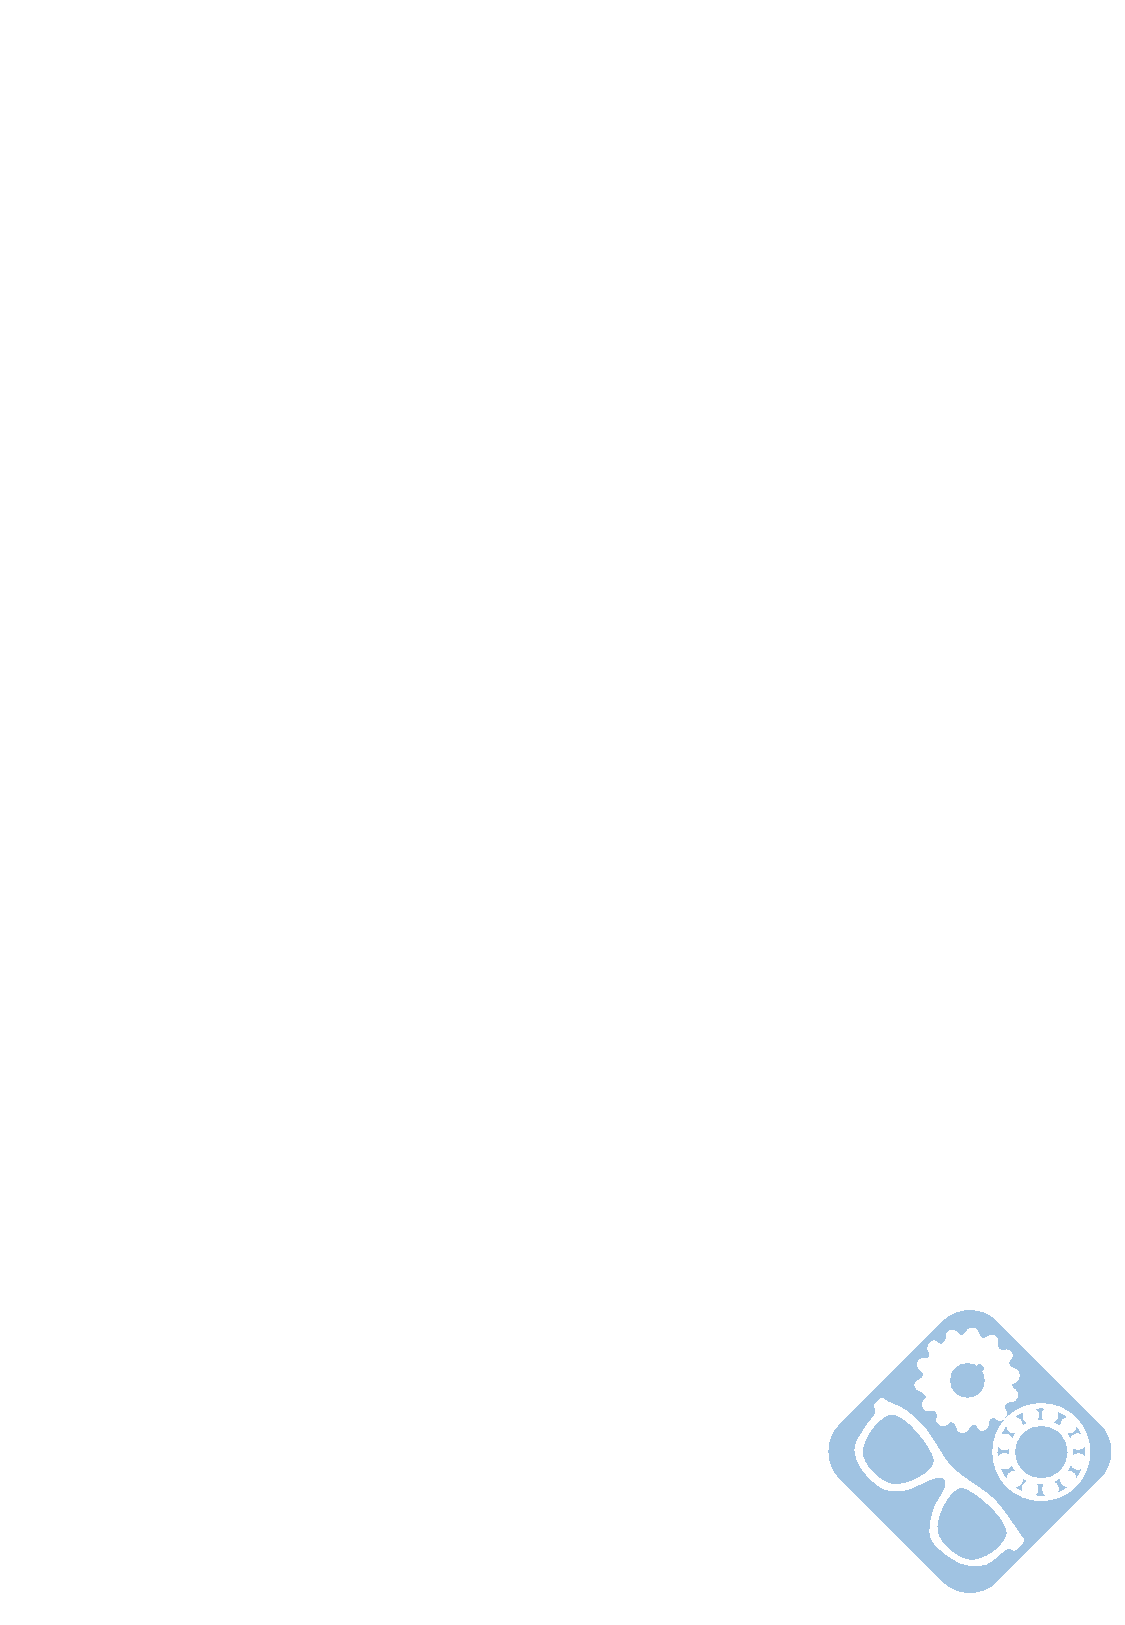
\includegraphics[width=\paperwidth,height=\paperheight,%
keepaspectratio]{../../img/fond4}%
\end{center}
\vfill
}}}

\begin{document}

\pagestyle{empty}

\AddToShipoutPicture*{\BackgroundPic}


\includegraphics[width=2cm]{../../img/logo}

\Huge{DS \num\ - \sujet}

\vspace{1cm}

\ifdef{\prive}{\begin{center}\colorbox{danger}{\Huge{Avec Correction}}\end{center}}{}

\begin{center}
\centering\huge{PTSI}
\end{center}

\vspace{2cm}


\begin{center}
\centering\Large{\jour}
\end{center}

\vspace{2cm}

\normalsize

\tableofcontents

\newpage

\AddToShipoutPicture{\BackgroundPicdeux}

\pagestyle{fancy}

\begin{center}
\Huge \sujet
\end{center}


\normalsize

\section{Système Spiralift pour salles modulables}

\subsection{Présentation générale}

\subsubsection{Salles modulables}

De nos jours, les organisateurs d'événements sont attachés à des prestations dont la qualité correspond au meilleur de ce que l'ingénierie peut offrir. Toutefois, les solutions architecturales et technologiques adaptées peuvent varier selon le type et l'ampleur de la manifestation : un concert de musique classique, un spectacle de danse, une conférence, un gala, ou un concert de musique amplifiée n'ont pas du tout les mêmes contraintes de sonorisation, d'acoustique, de disposition de
sièges, ou même de nombre de spectateurs assis...

Finalement, le seul point commun entre toutes ces activités est la nature très lourde des investissements nécessaires à la création de lieux adaptés.

Un autre constat s'impose aux responsables des collectivités territoriales : la fréquence de chaque type de manifestation justifie difficilement l'investissement nécessaire à l'édification d'une salle dédiée.

La solution la plus en vogue actuellement repose sur le principe de modularité : créer des salles modulables.

Les photos de la figure \ref{fig01} montrent quelques exemples de configurations possibles au Swisstech Convention Center de l'École Polytechnique Fédérale de Lausanne.


\begin{figure}[!h]
 \centering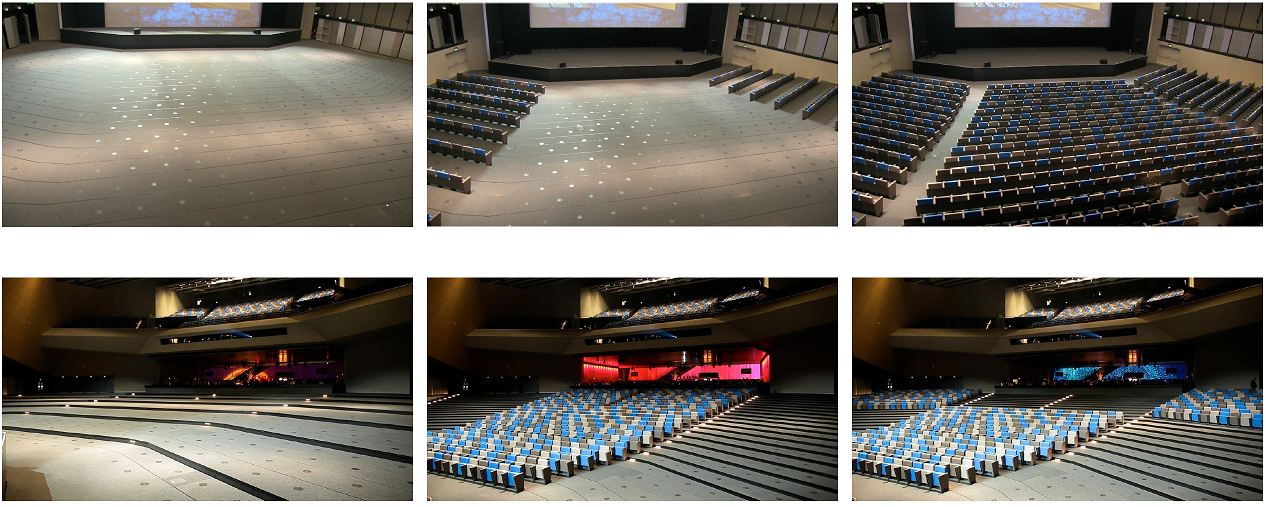
\includegraphics[width=0.7\linewidth]{img/fig01}
 \caption{Exemples de configurations}
 \label{fig01}
\end{figure}

Pour remplir pleinement son rôle, le système de transformation d'une telle salle se doit d'être flexible, simple d'utilisation et nécessiter peu d'intervention humaine. L'objectif est de transformer une salle en quelques heures afin de permettre la succession d'un maximum de manifestations dans un temps donné : un taux d'occupation élevé permet un amortissement rapide des investissements très lourds évoqués précédemment.

Une solution très prisée repose sur l'utilisation de plates-formes mobiles permettant de modifier la hauteur de sièges. Sur ces plates-formes, les rangées de sièges sont pivotantes. Le tout est motorisé et contrôlable par automate.

La figure \ref{fig02} montre l'exemple d'une salle dans une configuration de type \og banquet \fg (le sol est horizontal pour recevoir des tables de dîner) et une configuration de type « théâtre » où les sièges sont en gradins.

\begin{figure}[!h]
 \centering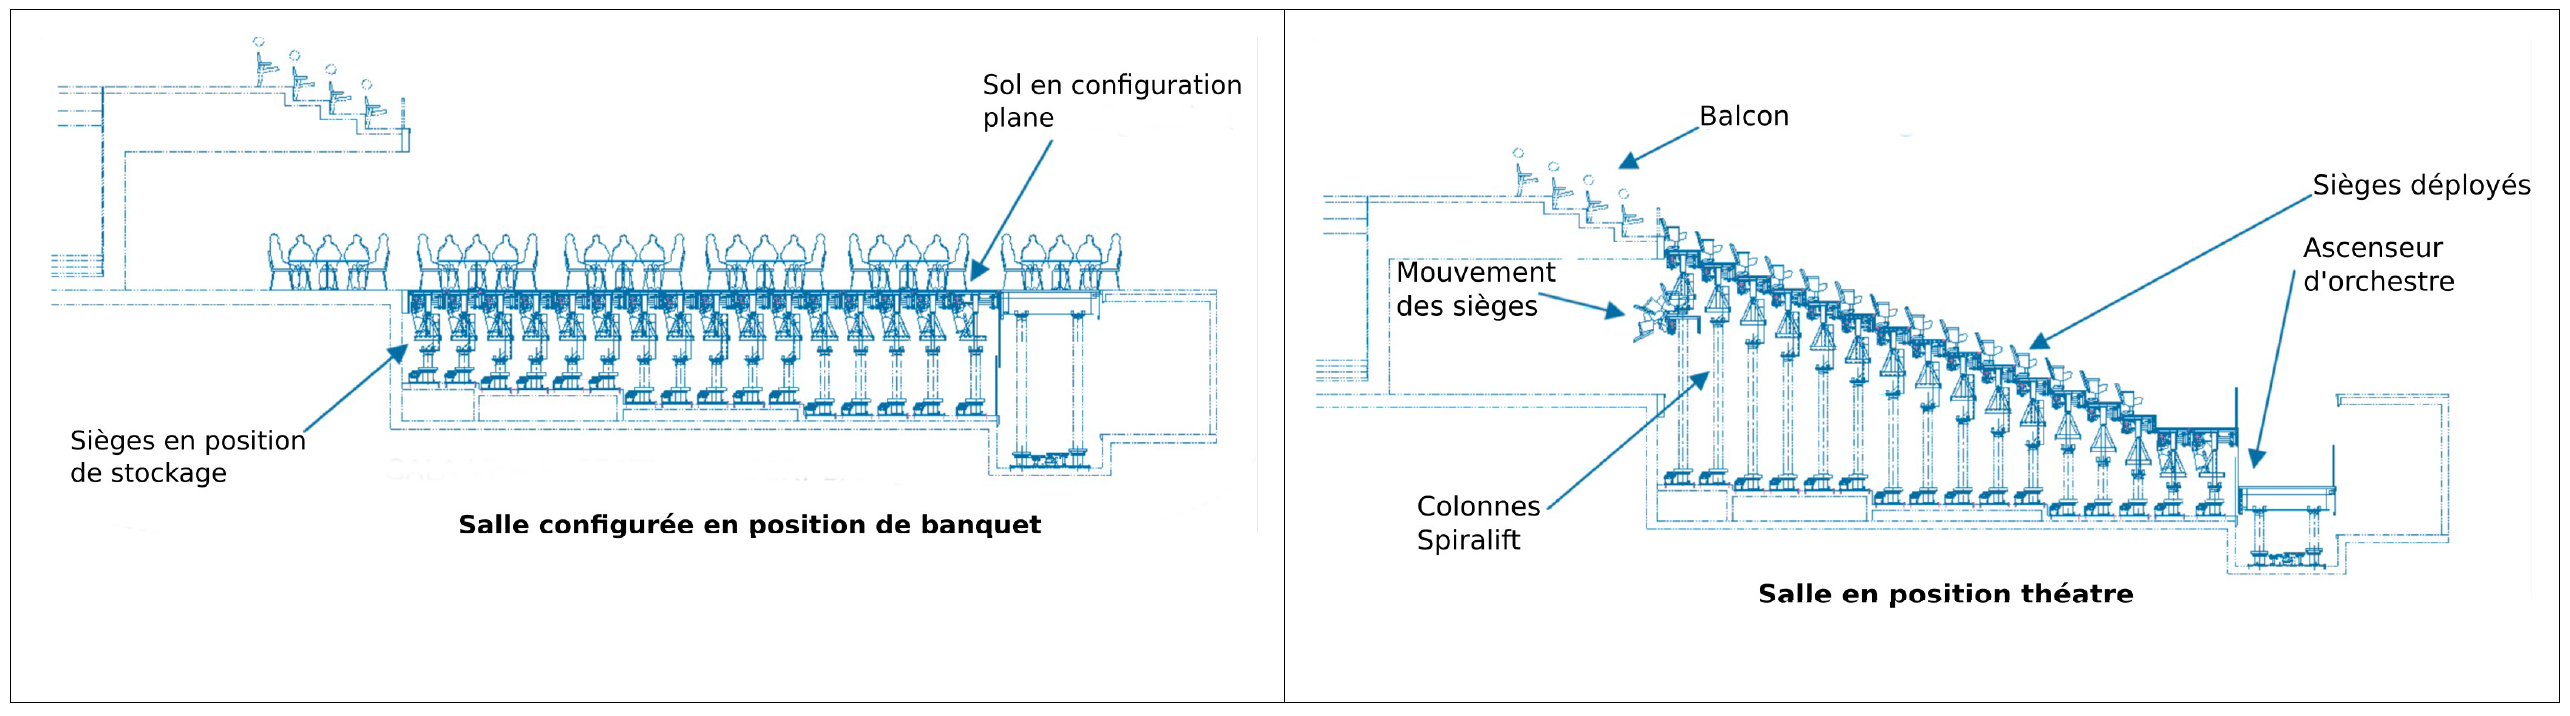
\includegraphics[width=0.7\linewidth]{img/fig02}
 \caption{Représentation des configurations \og banquet \fg et \og théâtre \fg}
 \label{fig02}
\end{figure}

La solution présentée ici et étudiée dans ce sujet repose sur l'utilisation des colonnes Spiralift de l'entreprise GALA SYSTEMES.

La figure \ref{fig03} montre une coupe transversale de deux rangées de sièges : les sièges de la rangée la plus haute sont déployés alors que ceux de l'autre rangée sont en position de stockage.

\begin{figure}[!h]
 \centering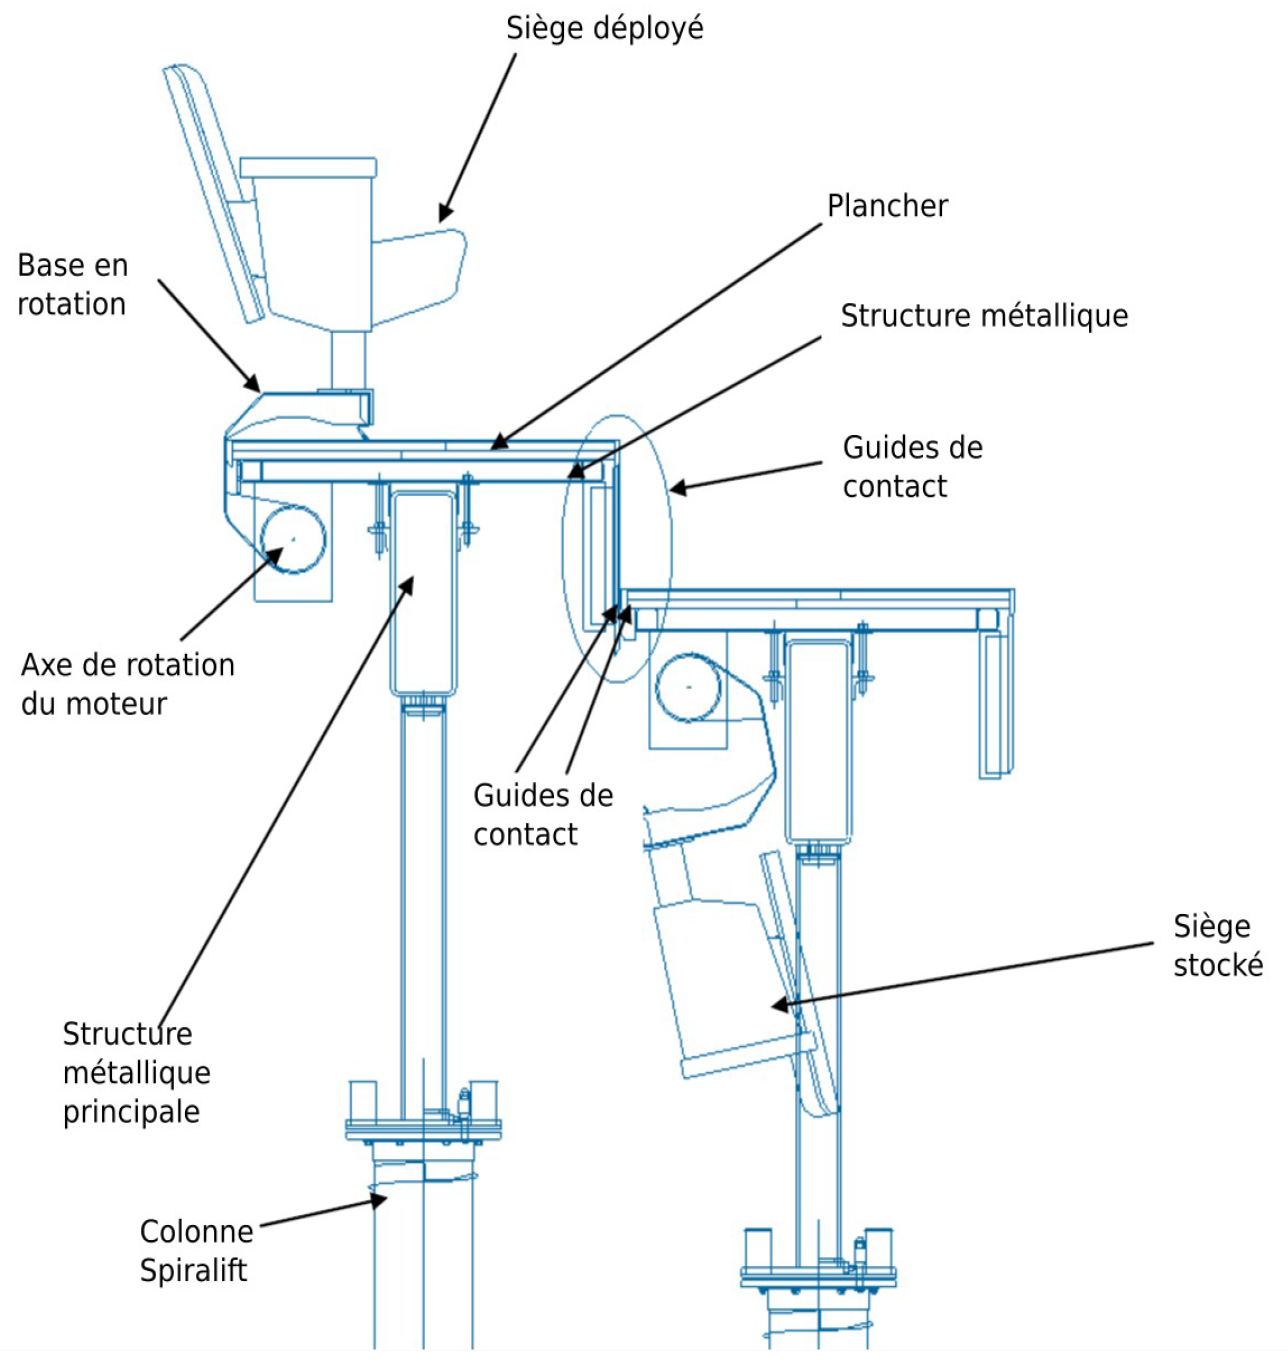
\includegraphics[width=0.7\linewidth]{img/fig03}
 \caption{Système de stockage des sièges}
 \label{fig03}
\end{figure}

Le déploiement des sièges se fait par rangée : l'ensemble des sièges d'une rangée est monté sur une base mobile en rotation par rapport à la structure métallique principale de cette rangée.

Un arbre, encastré avec cette base mobile, en liaison pivot par rapport à la structure métallique principale est actionné par des moteurs asynchrones.

Le mouvement vertical de l'ensemble {structure métallique principale + Plancher + Rangée de sièges} est obtenu grâce à des colonnes Spiralift décrites plus loin dans le sujet.

Cette solution permet d'obtenir une configuration de salle très flexible et évolutive car on peut obtenir des hauteurs de plancher quelconques, avec ou sans rangée de sièges.

Les sièges étant montés rigidement sur la base mobile en rotation, le type de siège choisi pour la salle n'est presque pas restreint par la solution technique de déploiement.

Hormis quelques contraintes d'encombrement et de poids, le décorateur peut choisir le type de siège qu'il souhaite, comme il le ferait dans une salle non-modulable.

\subsubsection{Motorisation des Spiralifts}

Dans la plupart des applications, les Spiralifts sont actionnés par des ensembles de moteur-freins, d'arbres de transmission et de réducteurs. Pour l'application considérée dans ce sujet, le schéma typique de la motorisation des Spiralifts est représenté par la figure \ref{fig04}.

\begin{figure}[!h]
 \centering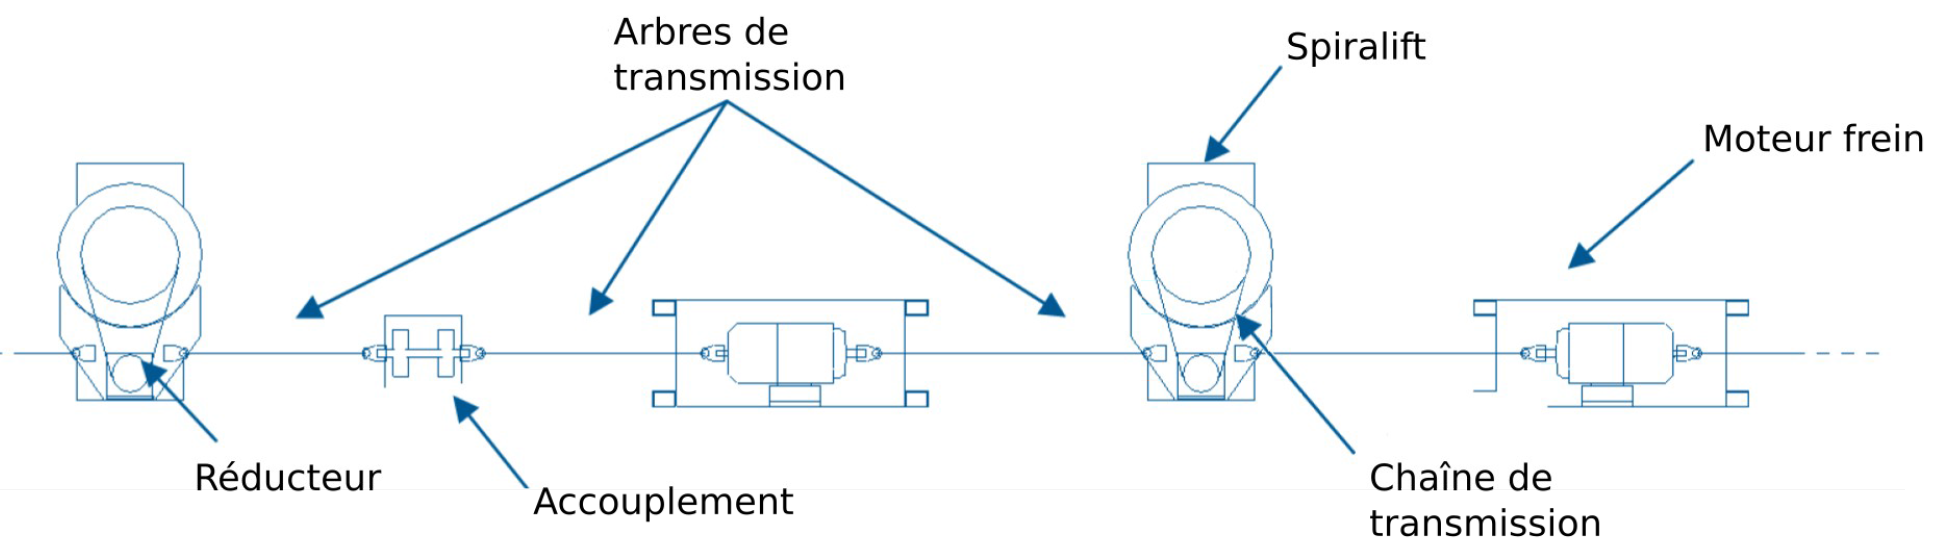
\includegraphics[width=0.7\linewidth]{img/fig04}
 \caption{Structure typique d'entraînement}
 \label{fig04}
\end{figure}

Pour des raisons de sécurité, comme c'est le cas de cette solution possédant deux moteurs-freins, les salles modulables sont équipées de systèmes placés en redondance (actionneurs, capteurs, éléments de transmission) pour pallier les éventuels dysfonctionnements.

Les caractéristiques de la chaîne d'action pilotant l'allée 26B (présentée en annexe 1) du Swisstech Convention Center sont données sur le diagramme de blocs internes représenté figure \ref{fig05}.

\begin{figure}[!h]
 \centering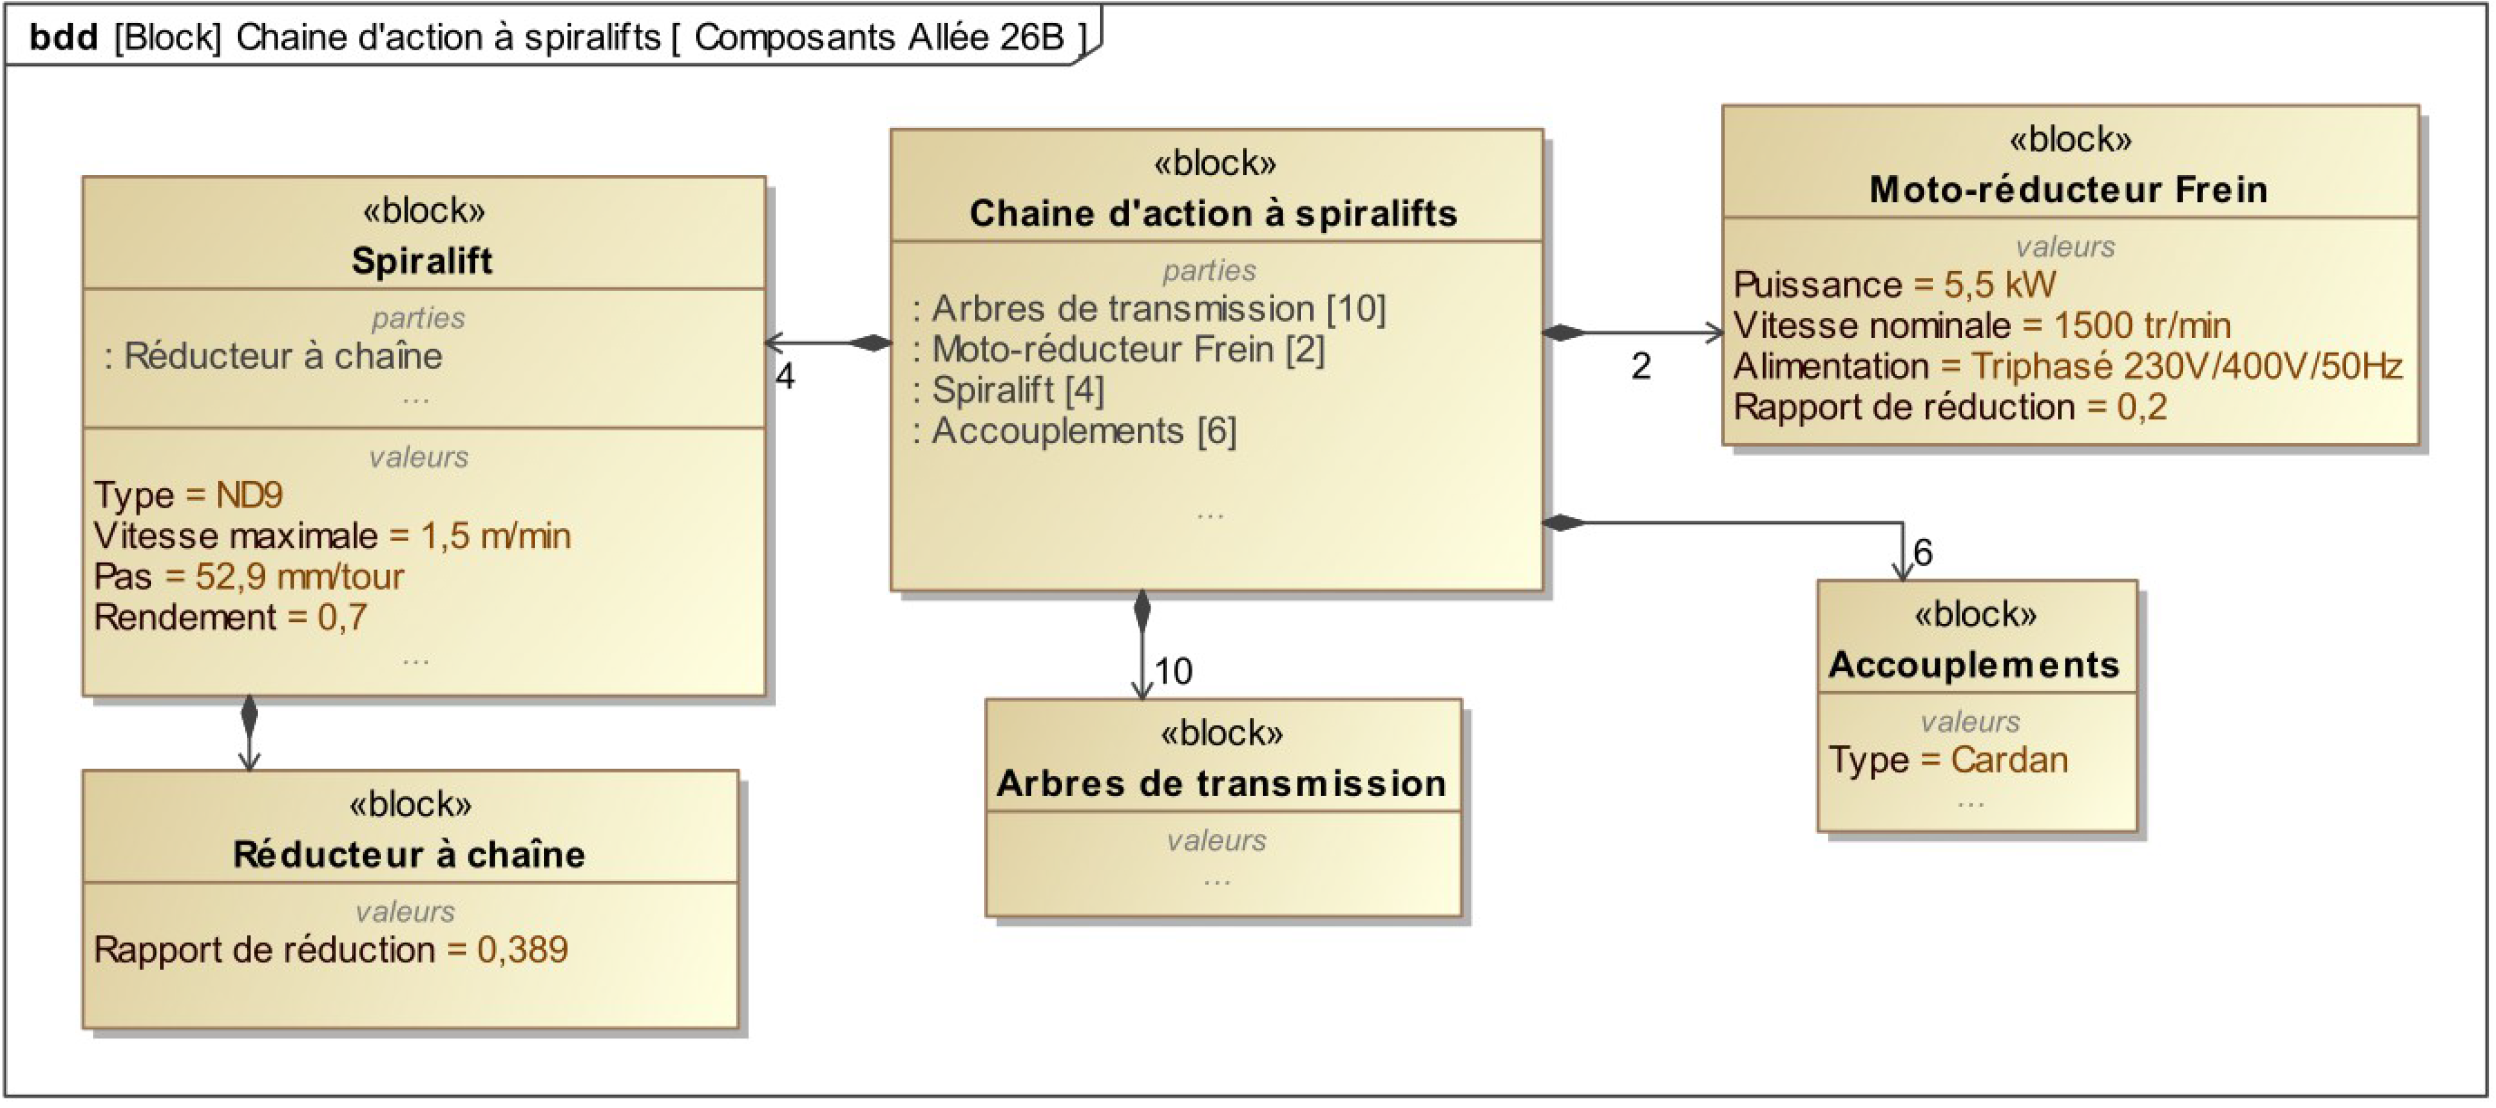
\includegraphics[width=0.7\linewidth]{img/fig05}
 \caption{Diagramme de blocs internes de la chaîne d'action à Spiralifts}
 \label{fig05}
\end{figure}

Les diagrammes SysML relatifs à l'installation d'une salle sont présentés sur les pages suivantes.

Le diagramme d'exigence partiel de la figure \ref{fig06} présente les contraintes imposées lors de la conception de la salle.

Le diagramme de la figure \ref{fig07} présente le détail des exigences liées à l'exigence Id=\og 13.1.2.3: plates-formes mobiles\fg.

Le diagramme de la figure \ref{fig08} présente les exigences relatives à l'asservissement de position de l'ascenseur d'orchestre.

\begin{figure}[!h]
 \centering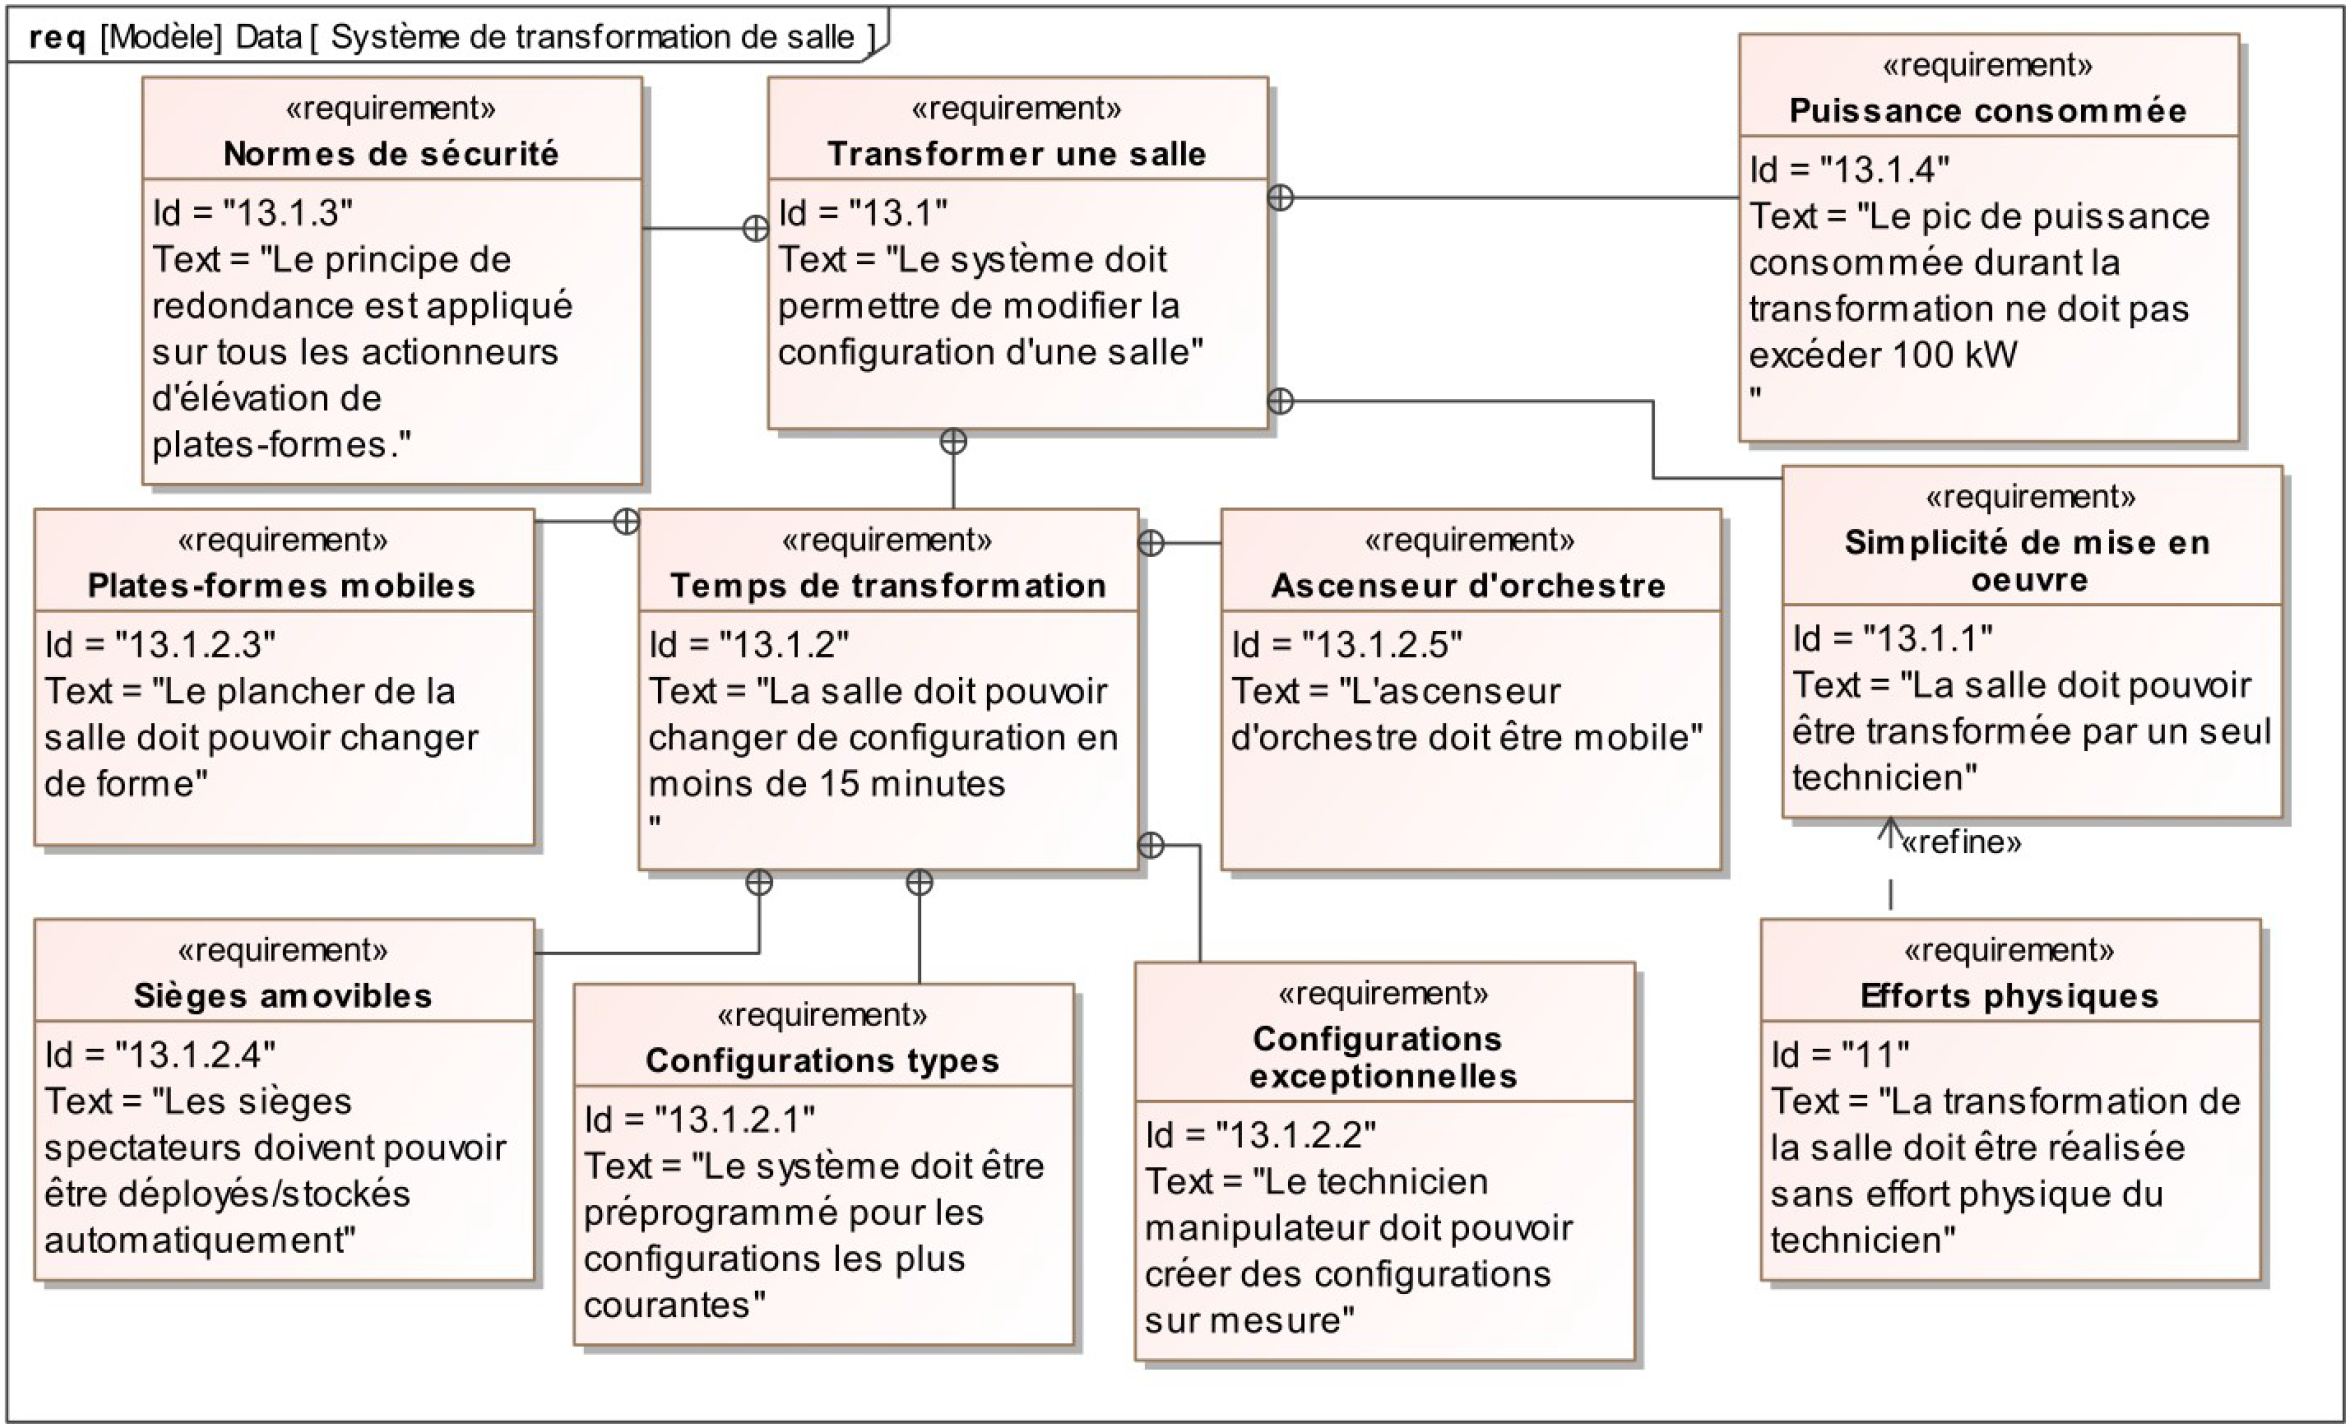
\includegraphics[width=0.7\linewidth]{img/fig06}
 \caption{Diagramme d'exigences de la transformation de la salle}
 \label{fig06}
\end{figure}

\begin{figure}[!h]
 \centering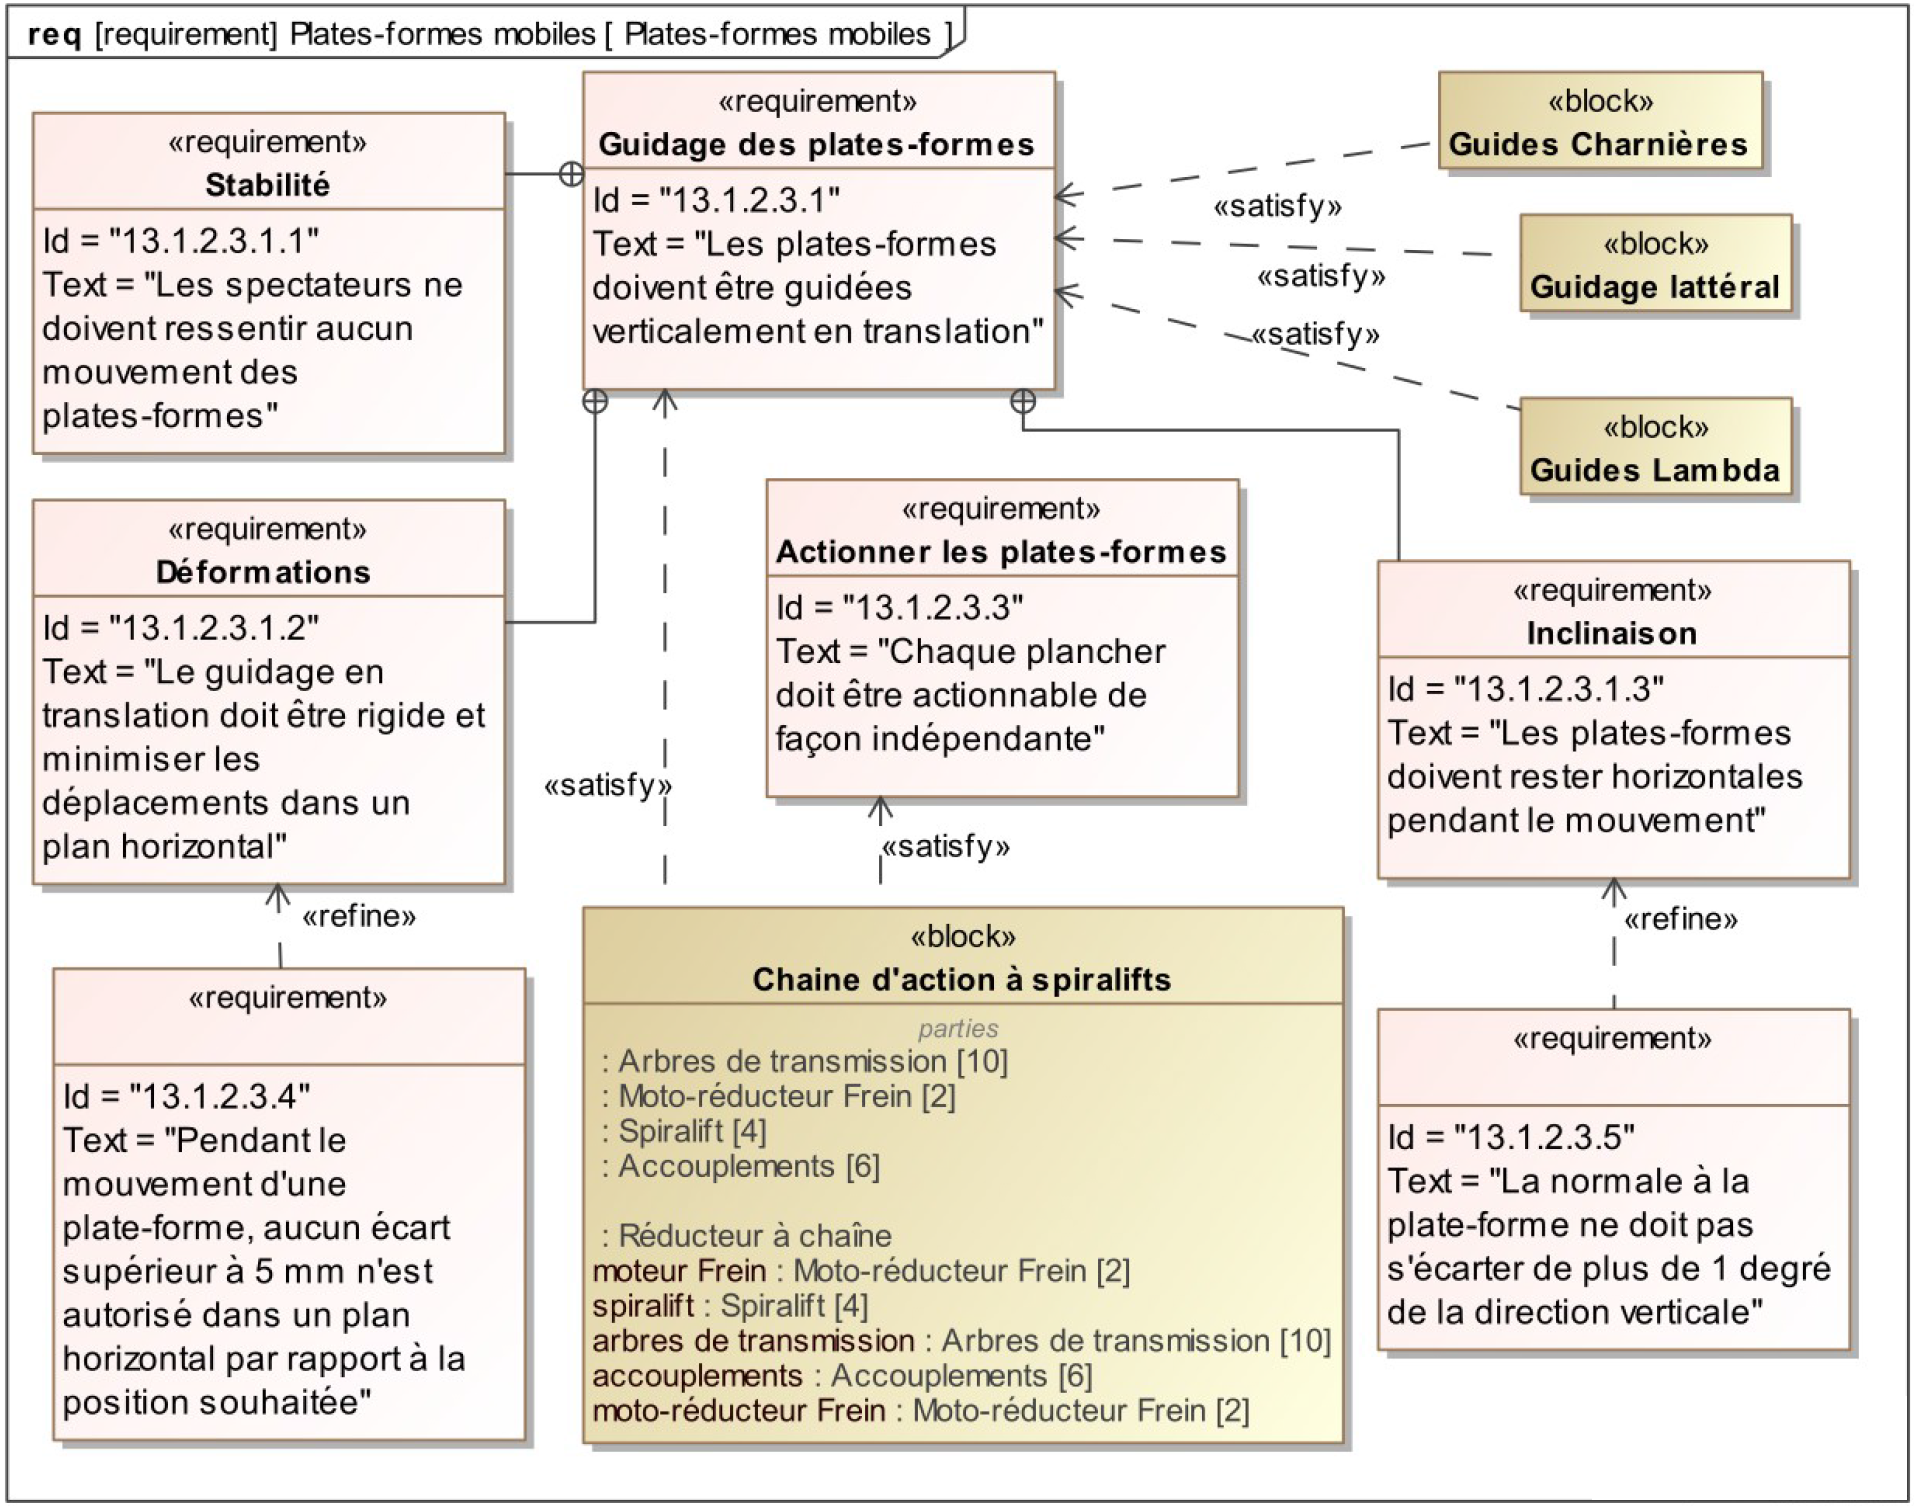
\includegraphics[width=0.7\linewidth]{img/fig07}
 \caption{Diagramme d'exigences du guidage des plates-formes}
 \label{fig07}
\end{figure}

\begin{figure}[!h]
 \centering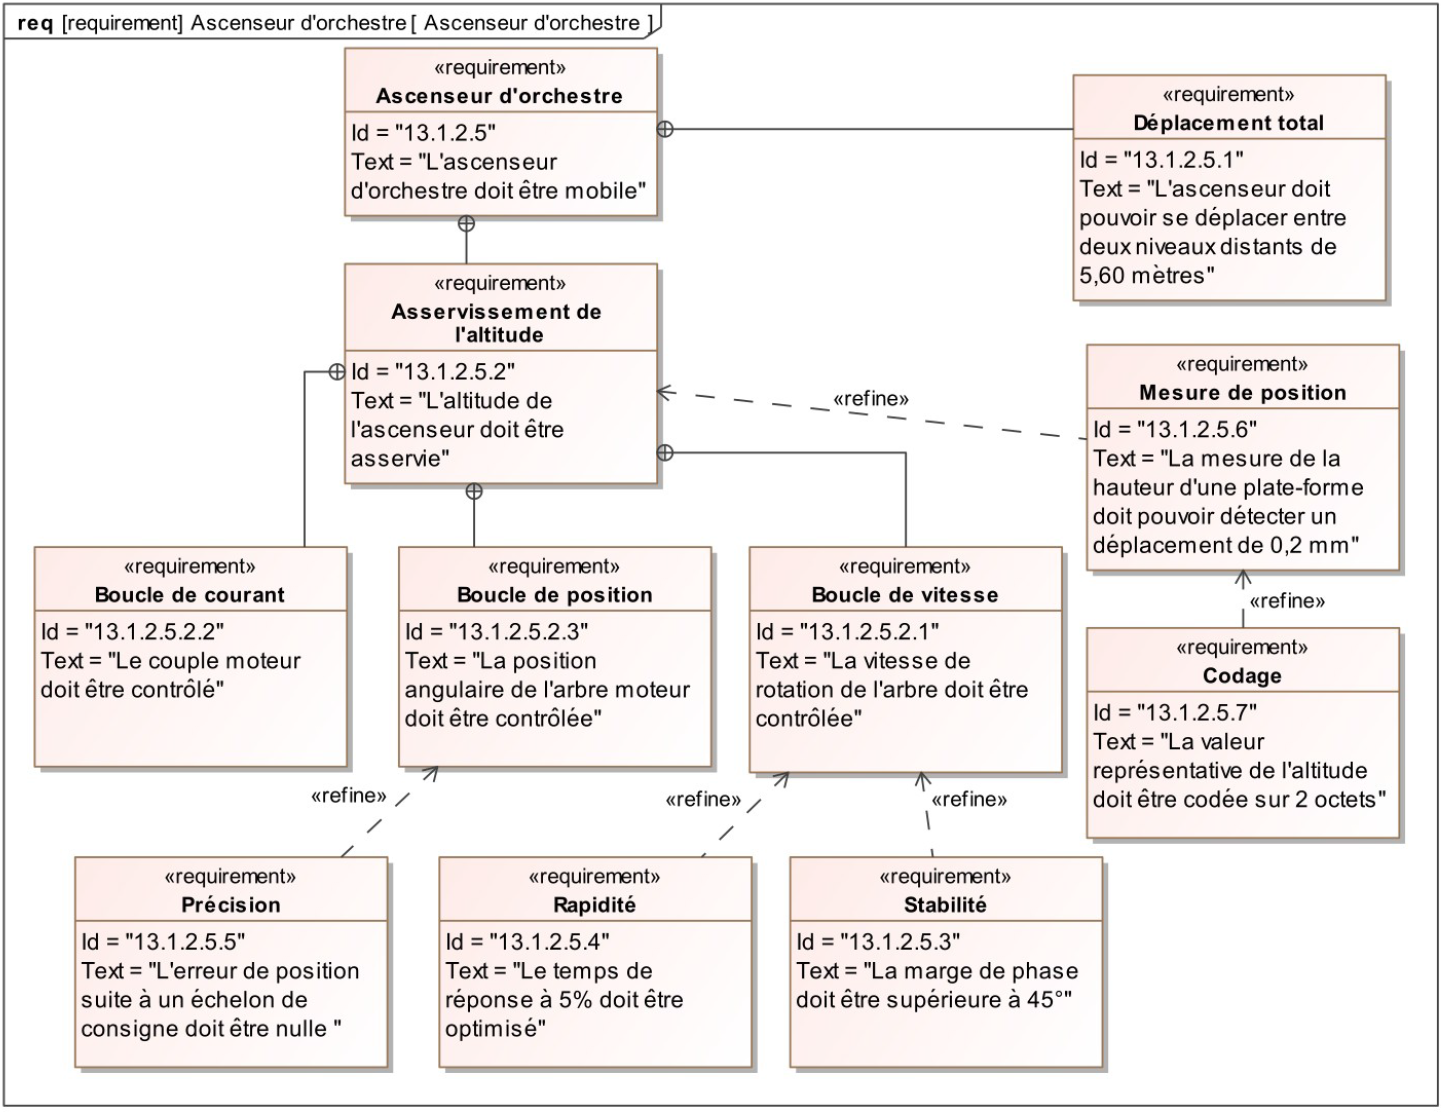
\includegraphics[width=0.7\linewidth]{img/fig08}
 \caption{Diagramme d'exigences du réglage de l'altitude de l'ascenseur d'orchestre}
 \label{fig08}
\end{figure}

\subsection{Objectifs}

Soucieuse de faire progresser ses solutions, une entreprise ayant l'habitude de proposer des salles sur la base de Spiralifts envisage quelques modifications à ses technologies habituelles. Afin de préparer ses prochaines études, elle décide de prendre comme base de réflexion la salle existante du Swisstech Convention Center de l'Ecole Polytechnique Fédérale de Lausanne.

\newpage

Cette étude est décomposée en six parties indépendantes :
\begin{itemize}
 \item dans la partie 1, on vérifiera les exigences relatives au guidage de la plate-forme d'une
rangée auto-guidée,
 \item dans la partie 2, on choisira la motorisation permettant le retournement d'une rangée de
sièges,
 \item dans la partie 3, on validera le choix du Spiralift (modèle et quantité) pour actionner une
plate-forme,
 \item dans la partie 4, on réglera l'asservissement de la position de l'ascenseur d'orchestre,
 \item dans la partie 5, on proposera une stratégie d'optimisation du temps de transformation d'une
salle, ce temps de transformation étant un critère important pour les exploitants de la salle,
 \item dans la partie 6, on réalisera un bilan global de l'étude.
\end{itemize}

\section{Solution technique pour assurer l'exigence de stabilité des planchers mobiles}

L'objectif de cette partie est de vérifier que les solutions de guidage retenues pour les plates-formes
mobiles permettent de garantir l'exigence de stabilité et de sécurité mentionnée dans le diagramme
d'exigence « plates-formes mobiles ».

Il existe principalement deux solutions de guidage des plates-formes mobiles :
\begin{itemize}
 \item \textbf{guidage mural} : lorsque les plates-formes sont en contact avec un mur de la salle, il est
possible de monter des rails de guidage dans les murs. On utilise alors des solutions
classiques de guidages linéaires à billes,
 \item \textbf{plate-forme auto-guidée} : lorsque les plates-formes sont au centre de la pièce, ou bien que
la solution de guidage mural est exclue (pour des considérations esthétiques par exemple), le
guidage peut être réalisé en utilisant des guides \og charnière \fg et \og lambda \fg.
\end{itemize}

La figure \ref{fig09} montre schématiquement l'agencement typique des différents composants assurant le guidage d'une plate-forme.

\begin{figure}[!h]
 \centering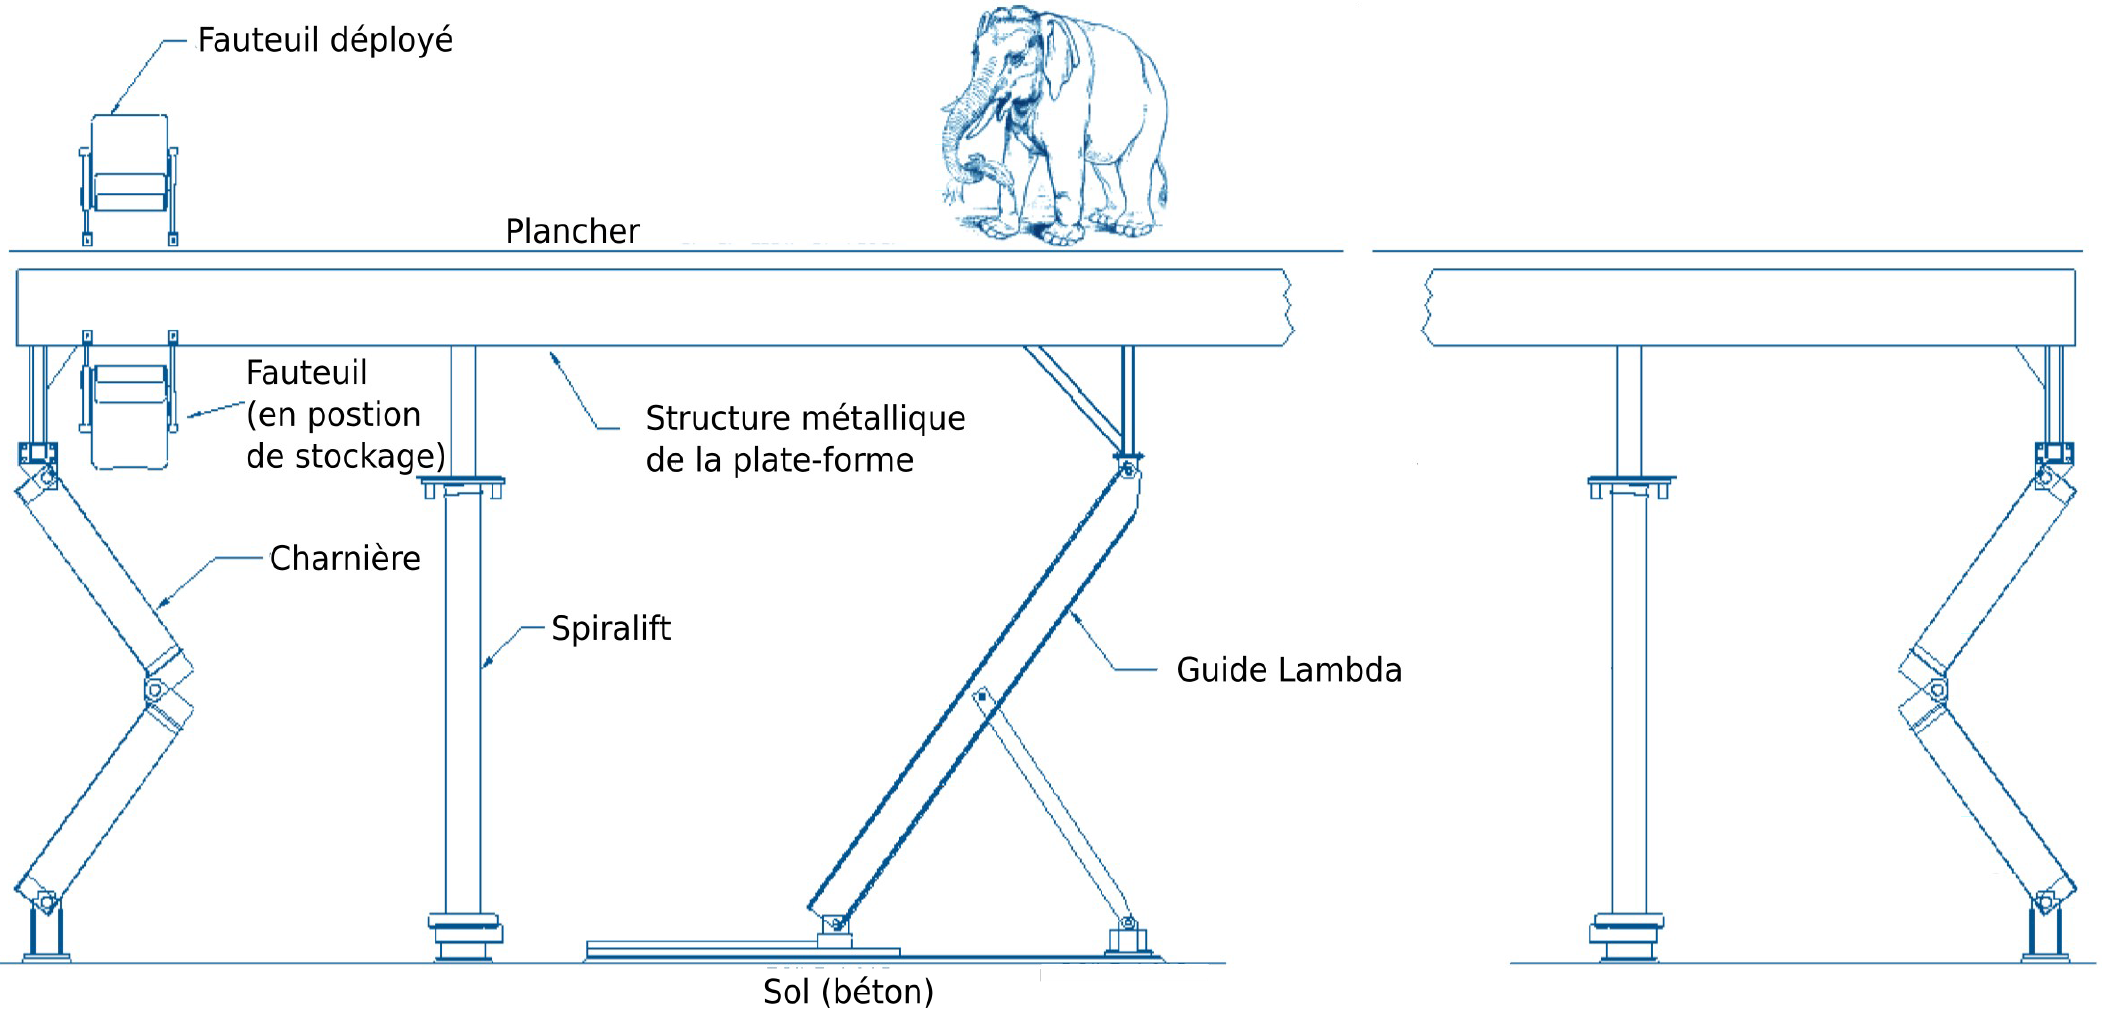
\includegraphics[width=0.7\linewidth]{img/fig09}
 \caption{Agencement typique du guidage d'une plate-forme}
 \label{fig09}
\end{figure}

Afin de bien se rendre compte des dimensions de ces composants, quelques vues complémentaires
d'une salle existante sont disponibles sur la figure \ref{fig10}.

\begin{figure}[!h]
 \centering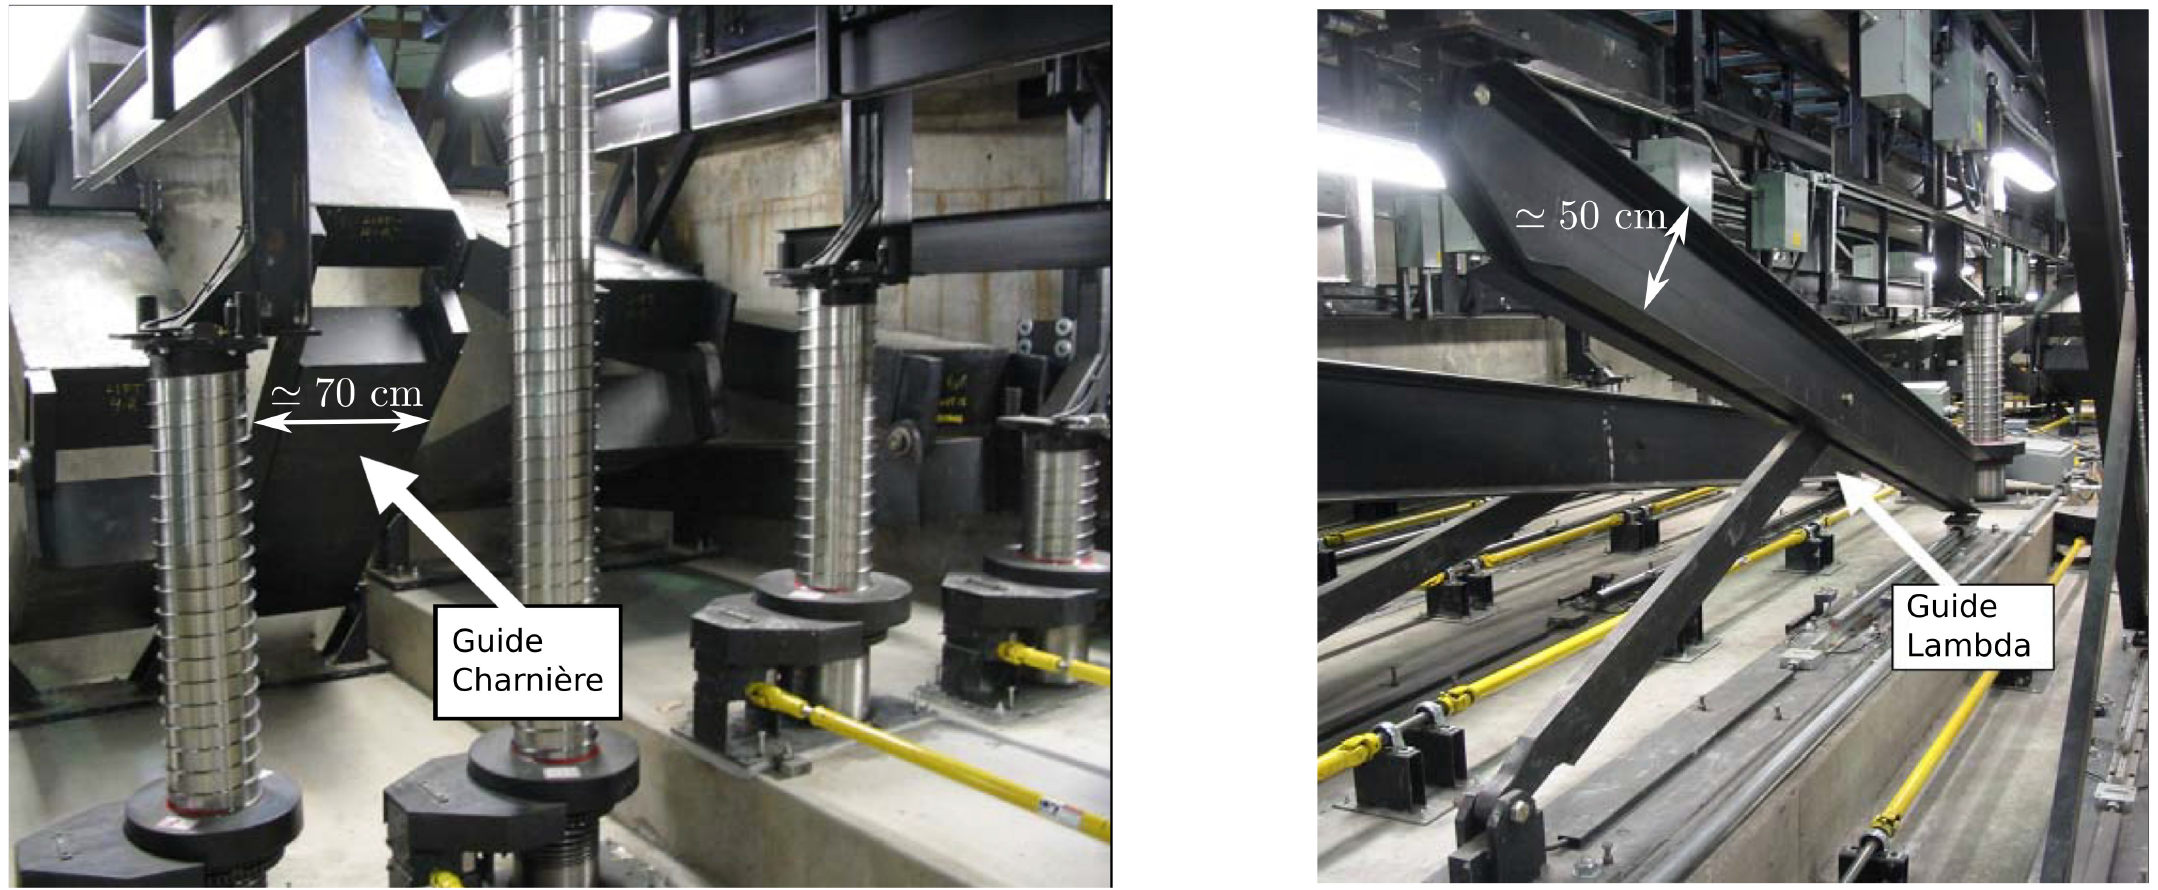
\includegraphics[width=0.7\linewidth]{img/fig10}
 \caption{Éléments de guidage d'une plate-forme}
 \label{fig10}
\end{figure}

Il est à noter que la plupart des modèles de Spiralift ne participent pas à la fonction de guidage, leur rôle étant seulement de transmettre un effort sur la plate-forme dans la direction verticale. La liaison entre un Spiralift et la plate-forme sera donc modélisée par une liaison ponctuelle.

On donne sur la figure \ref{fig11} le schéma cinématique du mécanisme de mise en mouvement vertical d'une plate-forme mobile.

\begin{figure}[!h]
 \centering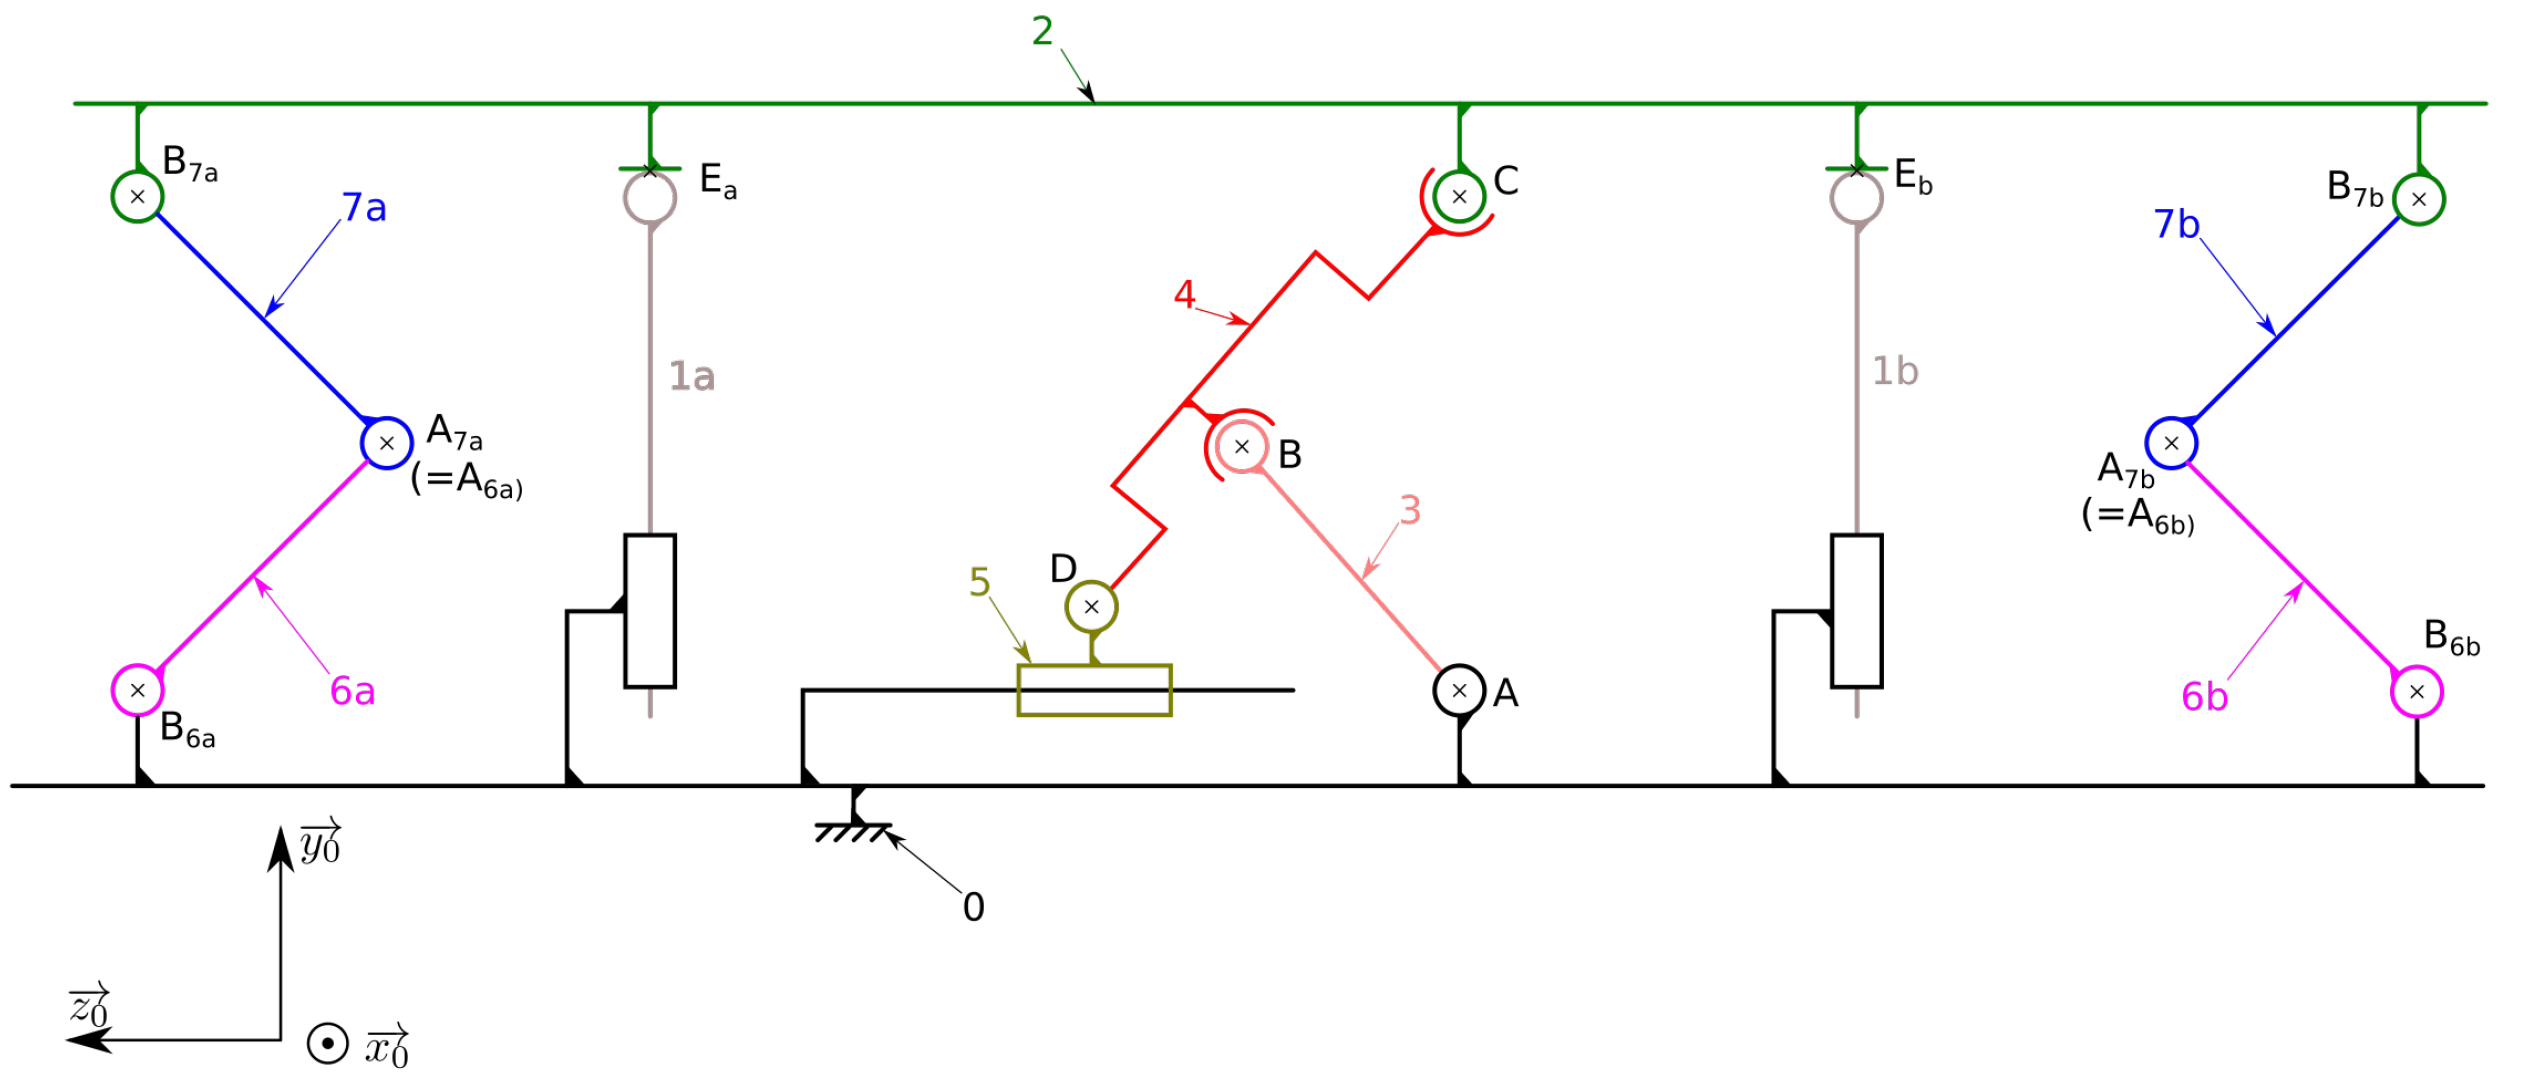
\includegraphics[width=0.7\linewidth]{img/fig11}
 \caption{Schéma cinématique du guidage d'une plate-forme}
 \label{fig11}
\end{figure}

Le sol est noté \textbf{0}. La plate-forme est notée \textbf{2}. Les deux guides charnières sont composés des pièces {\textbf{6a}, \textbf{7a}} et {\textbf{6b}, \textbf{7b}}. Le guide lambda est composé de \textbf{3}, \textbf{4}, et \textbf{5}.

Pour simplifier ce schéma, et puisque cette simplification n'a pas d'incidence sur l'analyse qui suit, le détail de la cinématique d'un Spiralift n'est pas représenté. Les deux Spiralifts sont donc représentés par \textbf{1a} et \textbf{1b}.

\question{Sur le document réponse, compléter le tableau en indiquant la désignation complète des liaisons (avec leurs caractéristiques telles que axes, centres, directions,...).}

\question{Dessiner le graphe de liaison de ce système.}

%\question{Conclure sur le respect de l'exigence « déformation » (Id=13.1.2.3.1.2 de la figure \ref{fig07}).}

Le guidage vertical d'une plate-forme par rapport au sol doit conduire à un mouvement descriptible par le tableau de mobilités suivant (par rapport au repère de la figure \ref{fig11}) :

\begin{center}
\begin{tabular}{|c|c|}
\hline
Rotations & Translations \\
\hline
$R_x=0$ & $T_x=0$ \\
\hline
$R_y=0$ & $T_y=1$ \\
\hline
$R_z=0$ & $T_z=0$ \\
\hline
\end{tabular}
\end{center}

\question{Montrer que $\overrightarrow{V_{C\in 2/0}}=\overrightarrow{V_{C\in 4/5}}+\overrightarrow{V_{C\in 5/0}}=\overrightarrow{V_{C\in 4/3}}+\overrightarrow{V_{C\in 3/0}}$.}

~\

Notations : le torseur cinématique du mouvement d'un solide \textbf{i} par rapport à un solide \textbf{j} exprimé au
point K dans une base $\left(\overrightarrow{x_n},\overrightarrow{y_n},\overrightarrow{z_n}\right)$ sera noté
$\left\{V_{i/j}\right\}=\left\{\begin{array}{c}\overrightarrow{\Omega_{i/j}}=\omega_{xij}\cdot \overrightarrow{x_n}+\omega_{yij}\cdot \overrightarrow{y_n}+\omega_{zij}\cdot \overrightarrow{z_n} \\
\overrightarrow{V_{K\in i/j}}=u_{ij}\cdot \overrightarrow{x_n}+v_{ij}\cdot \overrightarrow{y_n}+w_{ij}\cdot \overrightarrow{z_n}
\end{array}\right\}_K$

On prendra:
\begin{itemize}
 \item $\overrightarrow{CA}=-l(t)\cdot\overrightarrow{y_0}$,
 \item $\overrightarrow{CB}=l_1\cdot\overrightarrow{y_4}$,
 \item $\overrightarrow{CD}=l_2\cdot\overrightarrow{y_4}$. 
\end{itemize}

\question{A partir de la relation précédente, déterminer:\begin{itemize}
 \item une relation entre $w_{50}$, $l(t)$, $\omega_{30}$ et les paramètres géométriques,
 \item une relation entre $\omega_{43}$, $\omega_{45}$ et les paramètres géométriques.
\end{itemize}}

\question{Déterminer la relation qui lie $\omega_{43}$, $\omega_{45}$ et $\omega_{30}$.}

\question{En déduire le nombre de mobilités du sous-système \textbf{0}, \textbf{3}, \textbf{4} et \textbf{5}.}

\question{Déterminer le nombre de mobilités du système.}

\question{En détaillant bien votre raisonnement, déterminer le degré d'hyperstatisme du mécanisme modélisé sur le schéma cinématique.}

%\question{Dans le tableau du document réponse, indiquer par une croix la suppression d'un degré de liberté contribuant à la vérification d'une exigence « déformation » ou « inclinaison » (voir figure \ref{fig07}).}

\question{Compléter le tableau du document réponse, en indiquant d'une croix, le (ou les) composant(s) contribuant à la suppression d'un degré de liberté.}

%\question{Les solutions de guidage choisies sont-elles à même de supprimer l'ensemble des degrés de liberté nécessaires à la prise en compte des exigences « déformation » et « inclinaison » ?}

\section{Vérification des exigences relatives au retournement d'une rangée de sièges}

Le retournement d'une rangée de sièges s'effectue à l'aide d'une motorisation dont les caractéristiques sont résumées par la figure \ref{fig12}.
	
\begin{figure}[!h]
 \centering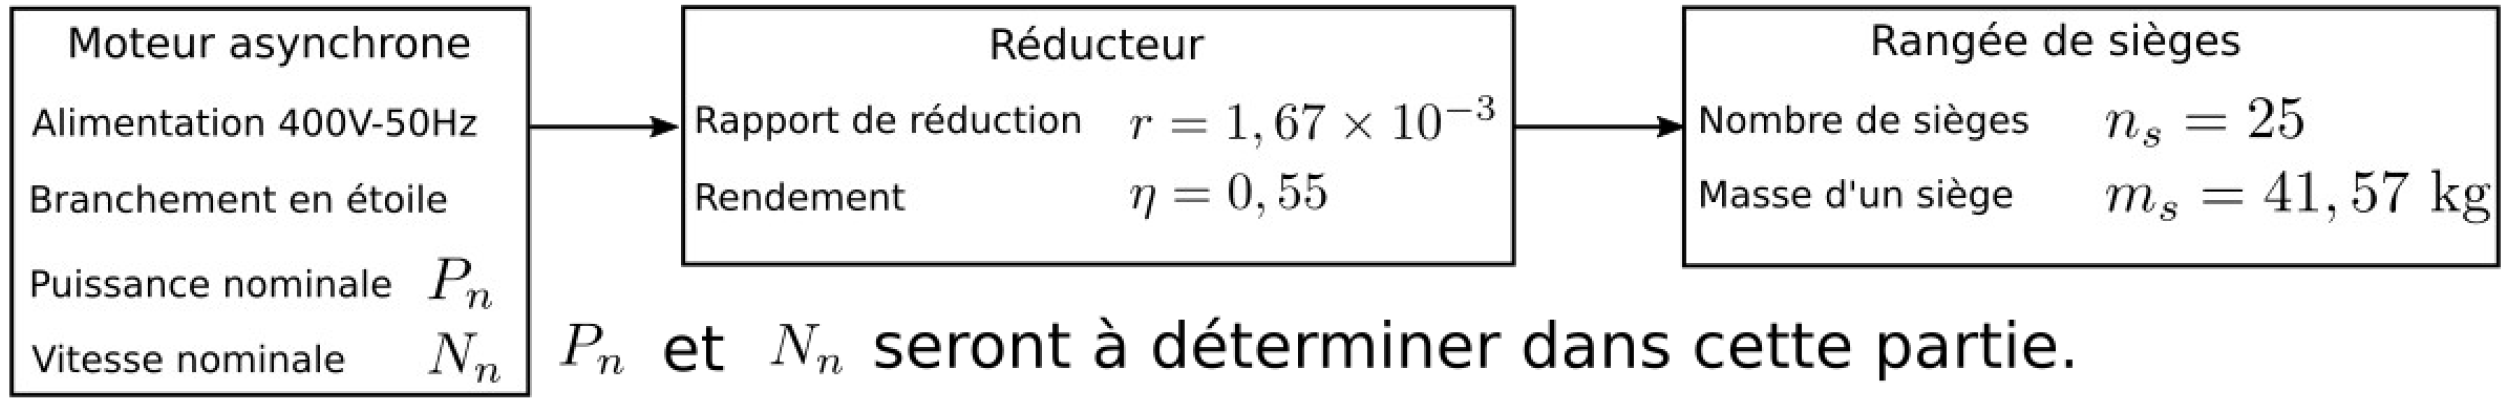
\includegraphics[width=0.7\linewidth]{img/fig12}
 \caption{Caractéristiques de la chaîne d'énergie du retournement des sièges}
 \label{fig12}
\end{figure}

La cinématique du retournement et le paramétrage utilisé dans cette partie sont décrits par la figure \ref{fig13} ci-dessous.

\begin{figure}[!h]
 \centering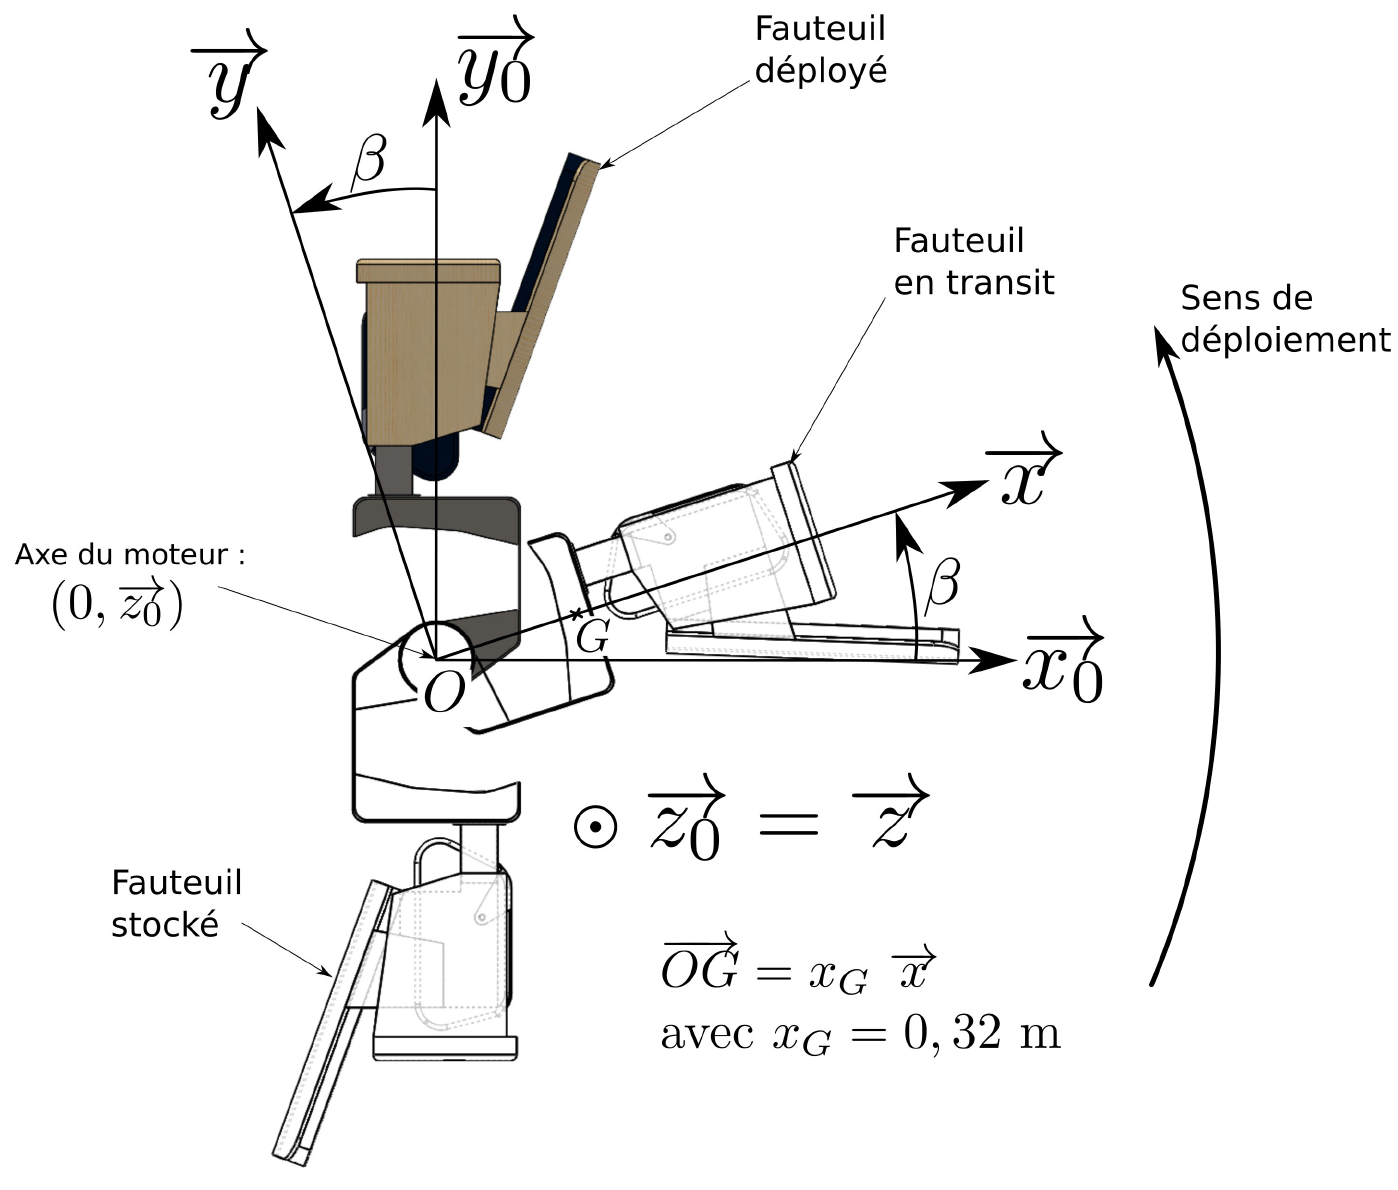
\includegraphics[width=0.7\linewidth]{img/fig13}
 \caption{Paramétrage du mouvement d'une rangée de sièges}
 \label{fig13}
\end{figure}

L'objectif de cette partie est de choisir un moto-réducteur à l'aide d'un extrait de catalogue constructeur. On déterminera alors le nombre maximal de rangées de sièges qu'il est possible de retourner simultanément tout en respectant l'exigence de puissance consommée (voir diagramme d'exigence de la figure \ref{fig06}).

Hypothèses :
\begin{itemize}
 \item le retournement des sièges ne s'effectuant que lorsque la plate-forme est immobile, on peut considérer que le référentiel associé au repère $(O,\overrightarrow{x_0},\overrightarrow{y_0},\overrightarrow{z_0})$ est galiléen,
 \item on prendra la valeur $g=9,81m.s^{-2}$ pour l'accélération de la pesanteur ($\overrightarrow{g}=-g.\overrightarrow{y_0}$),
 \item on supposera que toutes les liaisons autres que les liaisons internes au réducteur sont
parfaites,
 \item pour des raisons de symétrie le problème peut être considéré dans le plan $(O,\overrightarrow{x_0},\overrightarrow{y_0})$,
 \item le retournement d'une rangée de siège s'effectue sur un demi-tour à une vitesse de rotation $N_{max}=2,5tr.min^{-1}$,
 \item afin de simplifier l'étude, on considère que le couple à retenir pour le choix du moteur correspond au couple maximal déterminé par une étude statique.
\end{itemize}

\question{Déterminer la vitesse de rotation du moteur en tours par minute pour obtenir la vitesse $N_{max}$.}

%\question{Pour quel angle $\beta$ le couple à appliquer sur une rangée de sièges pour la maintenir en équilibre est-il maximal ?}

%\question{En déduire le couple maximal $Cm$ en sortie de moteur.}

%\question{À l'aide de la documentation fournie en annexe 2, choisir parmi les moteurs qui conviennent, celui dont la masse est la plus faible. Compléter la désignation de ce moteur sur le document réponse N°1.}

%\question{À partir de la documentation du moteur choisi, calculer la puissance active consommée pour retourner une rangée de sièges.}

%\question{En déduire le nombre de rangées de sièges qu'il est possible de retourner simultanément sans dépasser la puissance de 100kW imposée par le diagramme d'exigences de la figure \ref{fig06}.}

\section{Choix d'un modèle de Spiralift}

Dans cette partie, l'objectif est de valider le choix d'un modèle Spiralift, et de vérifier s'il est possible de réduire le nombre de Spiralifts nécessaires pour actionner l'allée 26B.

Cette étude va se dérouler en deux temps.

Dans un premier temps, nous allons déterminer si les efforts engendrés par les mouvements des guides ont une incidence prépondérante sur le dimensionnement d'un Spiralift. Pour cela, il va falloir réaliser :
\begin{itemize}
 \item une étude cinématique du mouvement des guides charnières,
 \item une étude dynamique liée à ce même mouvement pour déterminer les efforts à développer pour provoquer ce mouvement.
\end{itemize}

Dans un second temps, nous allons déterminer la charge sur un Spiralift.

\subsection{Présentation détaillée de la problématique}

Les guides charnières sont des pièces qui assurent la rigidité à l'ensemble d'une plate-forme mobile en mouvement. Pour cela, ce sont des pièces mécano-soudées de dimensions importantes. Les caractéristiques cinétiques des demi-charnières sont données en annexe 3.

Compte tenu des valeurs élevées de ces caractéristiques cinétiques, on peut s'interroger sur l'effort à développer pour imposer le mouvement de ces pièces.

\subsection{Paramétrage}

\begin{figure}[!h]
 \centering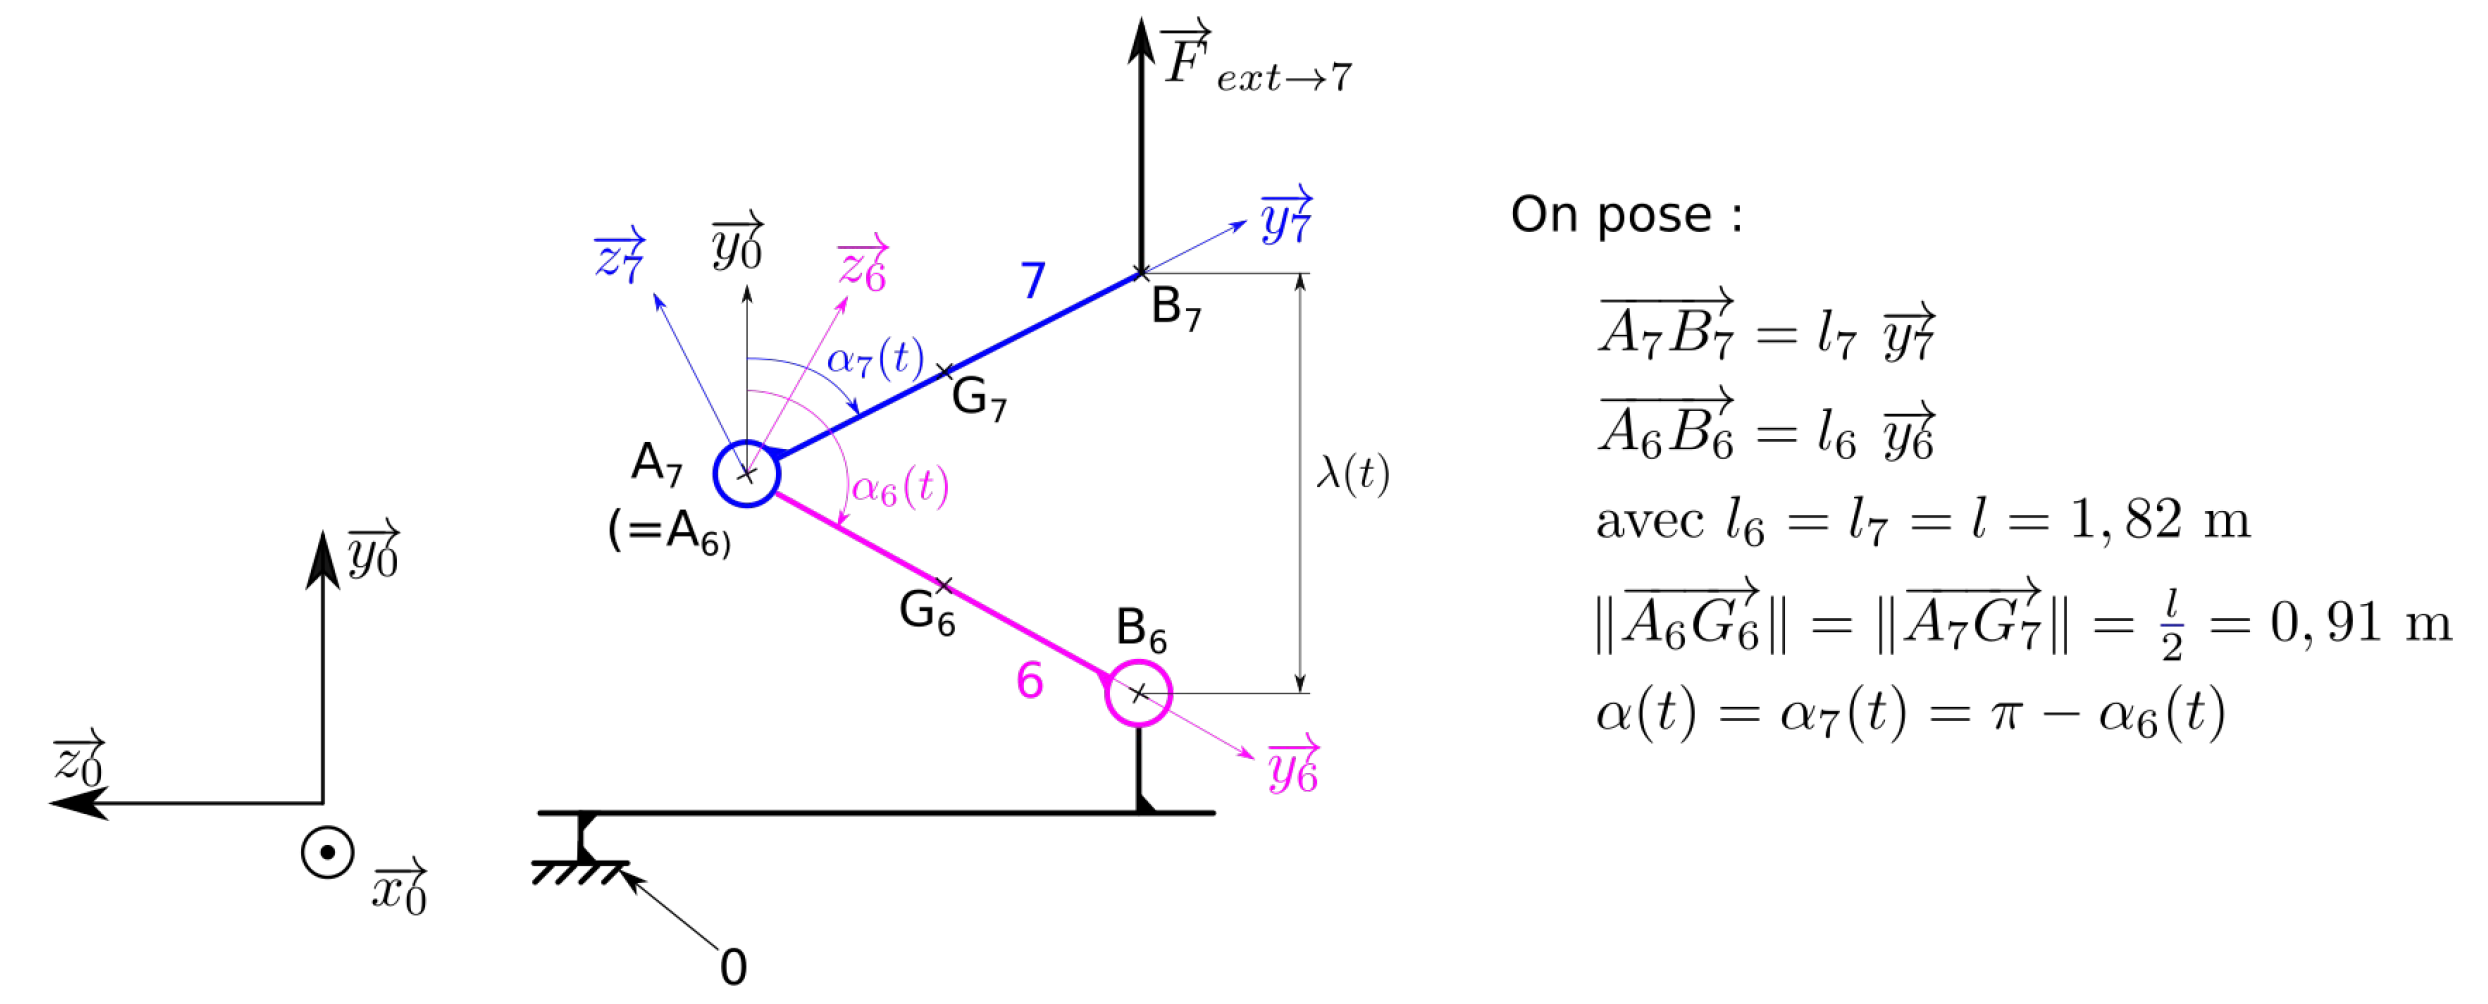
\includegraphics[width=0.7\linewidth]{img/fig14}
 \caption{Paramétrage du mouvement d'une charnière}
 \label{fig14}
\end{figure}

On considère l'ensemble \textbf{E}={\textbf{6}+\textbf{7}} qui représente un guide charnière. L'annexe 3 fournit les données sur chaque demi-charnière. Pour simplifier l'étude, on considérera que \textbf{6} et \textbf{7} sont identiques.

%L'objectif de cette partie est de déterminer la force $\overrightarrow{F_{ext\rightarrow 7}}=F.\overrightarrow{y_0}$ à exercer sur \textbf{7} en $B_7$ pendant le mouvement de la plate-forme.

Ce mouvement étant imposé, $\overrightarrow{B_6B_7}=\lambda(t).\overrightarrow{y_0}$ est supposé connu.

Pendant la montée, le mouvement de la plate-forme suit une loi de vitesse en trapèze.


\question{Le document réponse présente l'évolution de $\ddot{\lambda}\ (t)=\frac{1}{12}rad.s^{-1}$ et $\dot{\lambda}\ (t)$. Tracer $\lambda\ (t)$ en sachant que $\lambda\ (0)=0$. On fera particulièrement attention:
\begin{itemize}
 \item aux valeurs initiale et finale de $\lambda$,
 \item à l'allure générale de la courbe.
\end{itemize}}

\subsection{Relation entre $\lambda(t)$ et $\alpha(t)$}

Pour la suite de l'étude, nous aurons besoin de la relation mathématique liant $\lambda(t)$ et $\alpha(t)$ qui pourront être notées  $\lambda$ et $\alpha$ pour simplifier les notations.

\question{À l'aide d'une relation de fermeture géométrique, montrer que $\lambda=2\cdot l\cdot cos(\alpha)$.}

~\

La figure \ref{fig14a} présente plusieurs courbes dont l'une représente $\alpha\ (t)$.

\begin{figure}[!h]
 \centering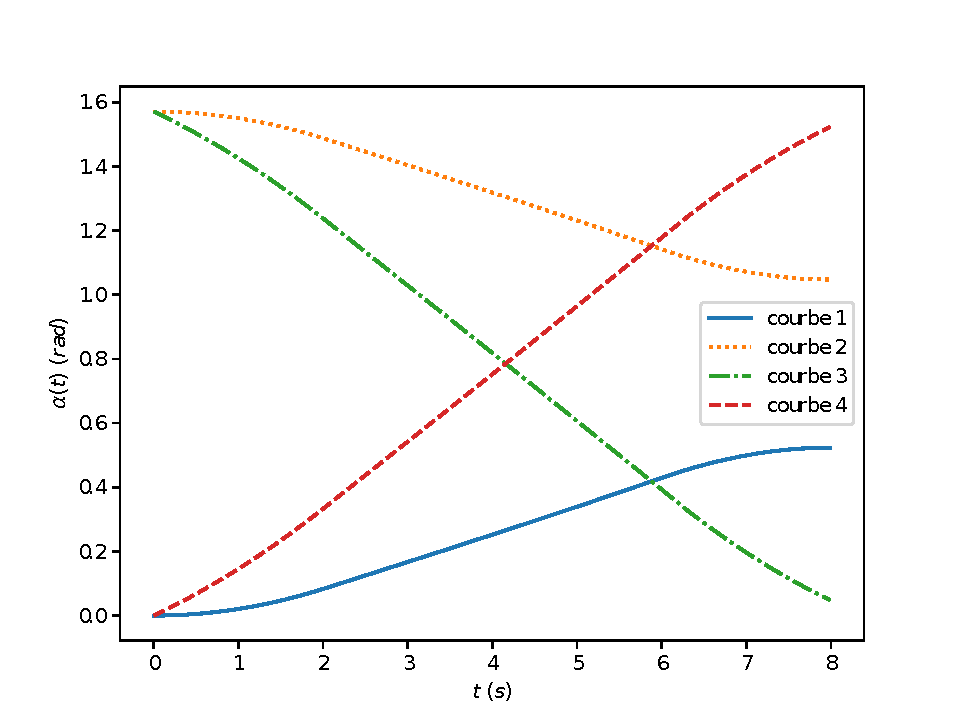
\includegraphics[width=0.7\linewidth]{img/fig14a}
 \caption{Évolution de $\alpha\ (t)$}
 \label{fig14a}
\end{figure}

\question{Déterminer à quelle courbe (1, 2, 3 ou 4) correspond $\alpha\ (t)$.}

\subsection{Détermination des torseurs cinématiques des mouvements de 6/0 et 7/0}

Dans toute la suite du problème, on fera l'hypothèse que le problème peut être traité comme un problème plan.

Notations : le torseur cinématique du mouvement d'un solide \textbf{i} par rapport à un solide \textbf{j} exprimé au
point K dans une base $\left(\overrightarrow{x_n},\overrightarrow{y_n},\overrightarrow{z_n}\right)$ sera noté
$\left\{V_{i/j}\right\}=\left\{\begin{array}{c}\overrightarrow{\Omega_{(i/j)}}=\omega_{ij}\cdot \overrightarrow{x_n} \\
\overrightarrow{V_{K,i/j}}=v_{ij}\cdot \overrightarrow{y_n}+w_{ij}\cdot \overrightarrow{z_n}
\end{array}\right\}_K$

\question{Exprimer le torseur cinématique du mouvement de \textbf{6} par rapport à \textbf{0} $\left\{V_{6/0}\right\}$ en $B_6$ en fonction de $\dot{\alpha}=\frac{d\alpha}{dt}$. En déduire l'expression de ce torseur en $G_6$.}

\question{Exprimer le torseur cinématique du mouvement de \textbf{7} par rapport à \textbf{0} $\left\{V_{7/0}\right\}$ en $B_7$ en fonction de $\dot{\alpha}=\frac{d\alpha}{dt}$, $\dot{\lambda}=\frac{d\lambda}{dt}$ et $l$. En déduire l'expression de ce torseur en $G_7$.}


\section{Asservissement de l'altitude d'une plate-forme de l'ascenseur d'orchestre}

Certaines salles sont équipées d'espaces de rangement situés sous la scène. Une plate-forme d'ascenseur d'orchestre peut s'abaisser au niveau du plancher de l'espace de stockage permettant ainsi à des opérateurs de faire glisser sur la plate-forme le matériel de scène, comme des décors ou des instruments de musique.

\begin{figure}[!h]
 \centering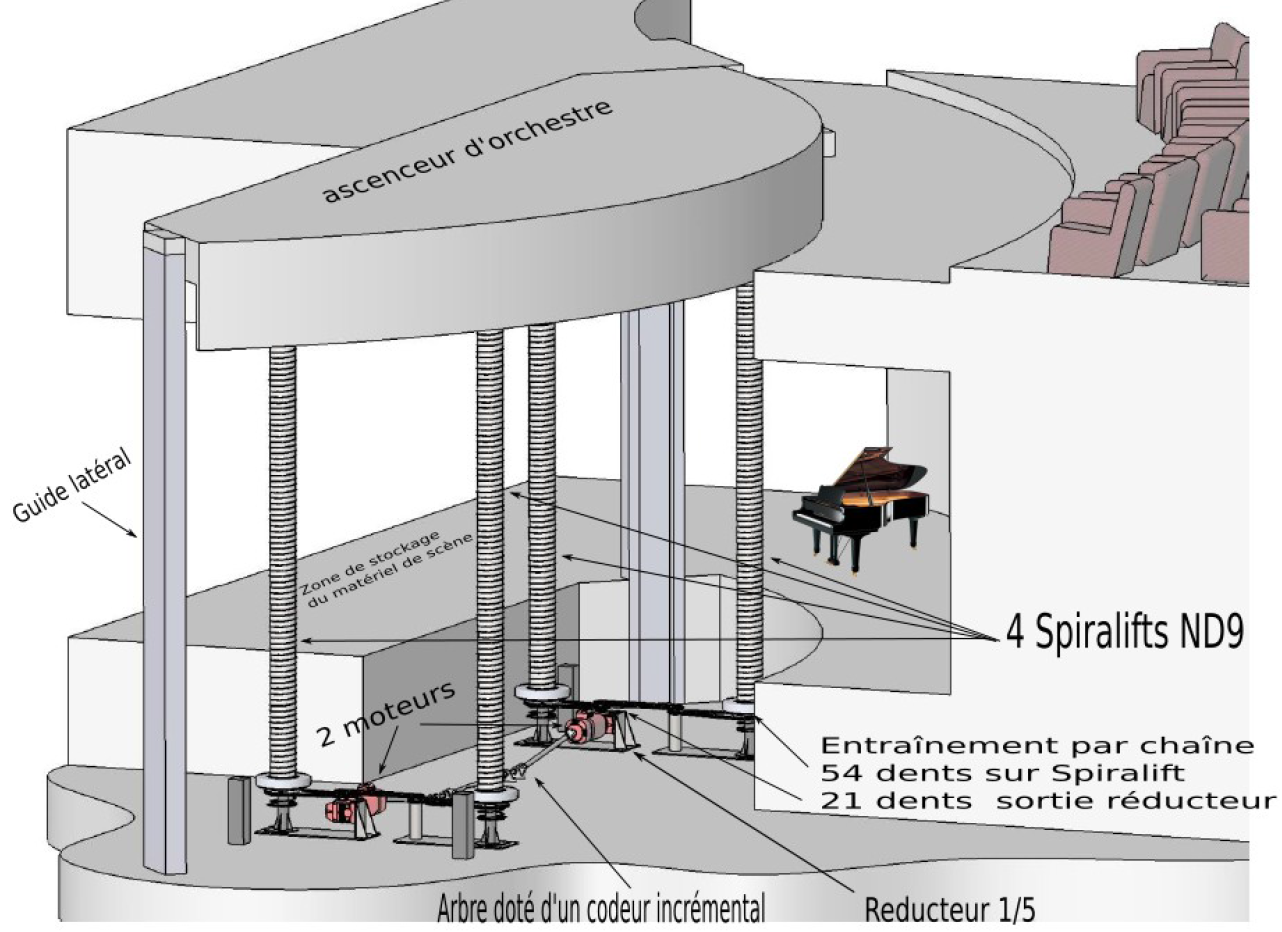
\includegraphics[width=0.7\linewidth]{img/fig16}
 \caption{Description de l'ascenseur d'orchestre}
 \label{fig16}
\end{figure}

Le positionnement de cette plate-forme doit être effectué avec une grande précision, afin de permettre le déploiement du matériel de scène par roulage entre l'espace de stockage et l'ascenseur d'orchestre.

L'étude qui suit se limitera à l'étude d'un seul moteur pilotant une seule colonne Spiralift.

Afin de modéliser l'asservissement de l'altitude de la plate-forme d'ascenseur d'orchestre, un schéma de cet asservissement a été développé. Ce schéma est présenté sur la figure \ref{fig17}.

\begin{figure}[!h]
 \centering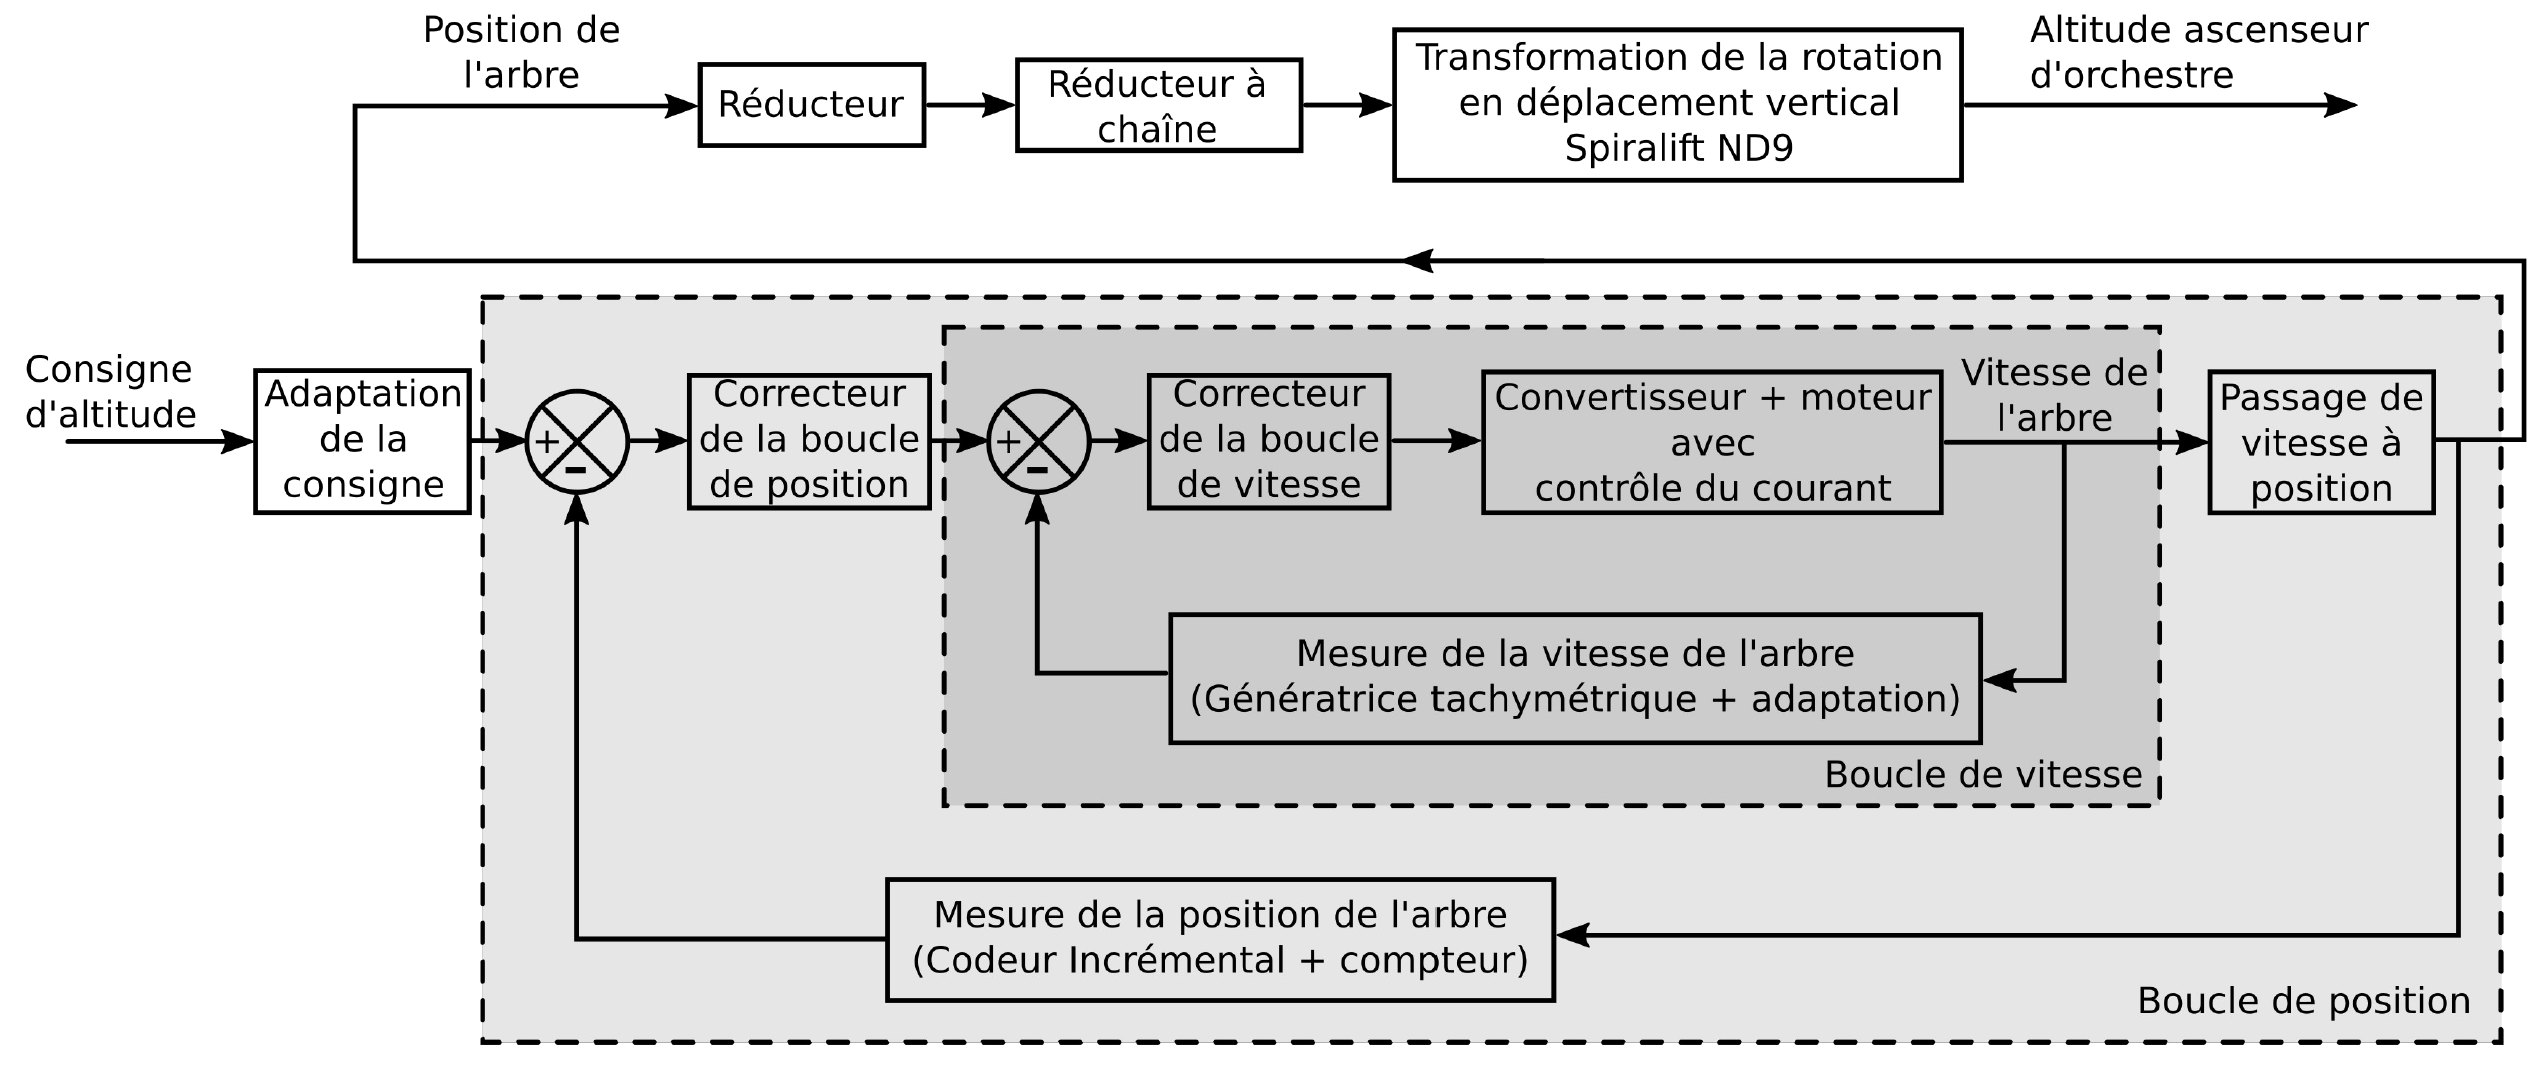
\includegraphics[width=0.7\linewidth]{img/fig17}
 \caption{Modélisation de l'asservissement d'altitude de l'ascenseur d'orchestre}
 \label{fig17}
\end{figure}

Dans une première partie de cette étude, l'objectif est de régler le correcteur de la boucle de vitesse, afin de satisfaire l'exigence de stabilité de cette boucle tout en optimisant son temps de réponse à 5\%.

Dans une deuxième partie, l'objectif sera de vérifier que les exigences de précisions relatives à l'asservissement de l'altitude de la plate-forme sont respectées.

Dans une troisième partie l'objectif sera de vérifier que la résolution du capteur d'altitude permet de répondre aux exigences attendues en matière d'affichage de l'altitude.

\subsection{Étude de la boucle de vitesse}

Afin d'assurer le bon positionnement de la plate-forme de l'ascenseur d'orchestre, le concepteur a choisi de contrôler la vitesse de l'arbre d'entraînement du Spiralift par le biais d'une boucle de vitesse.

Les objectifs de cette étude sont :
\begin{itemize}
 \item d'identifier les paramètres d'un modèle correspondant à la boucle de vitesse de l'arbre,
 \item de régler le correcteur à action proportionnelle de cette boucle de vitesse,
 \item de vérifier que les exigences de stabilité et d'optimisation du temps de réponse à 5\% de cette boucle de vitesse sont satisfaites.
\end{itemize}

Le schéma simplifié de la boucle de vitesse de l'arbre est donné sur la figure \ref{fig18}:
\begin{figure}[!h]
 \centering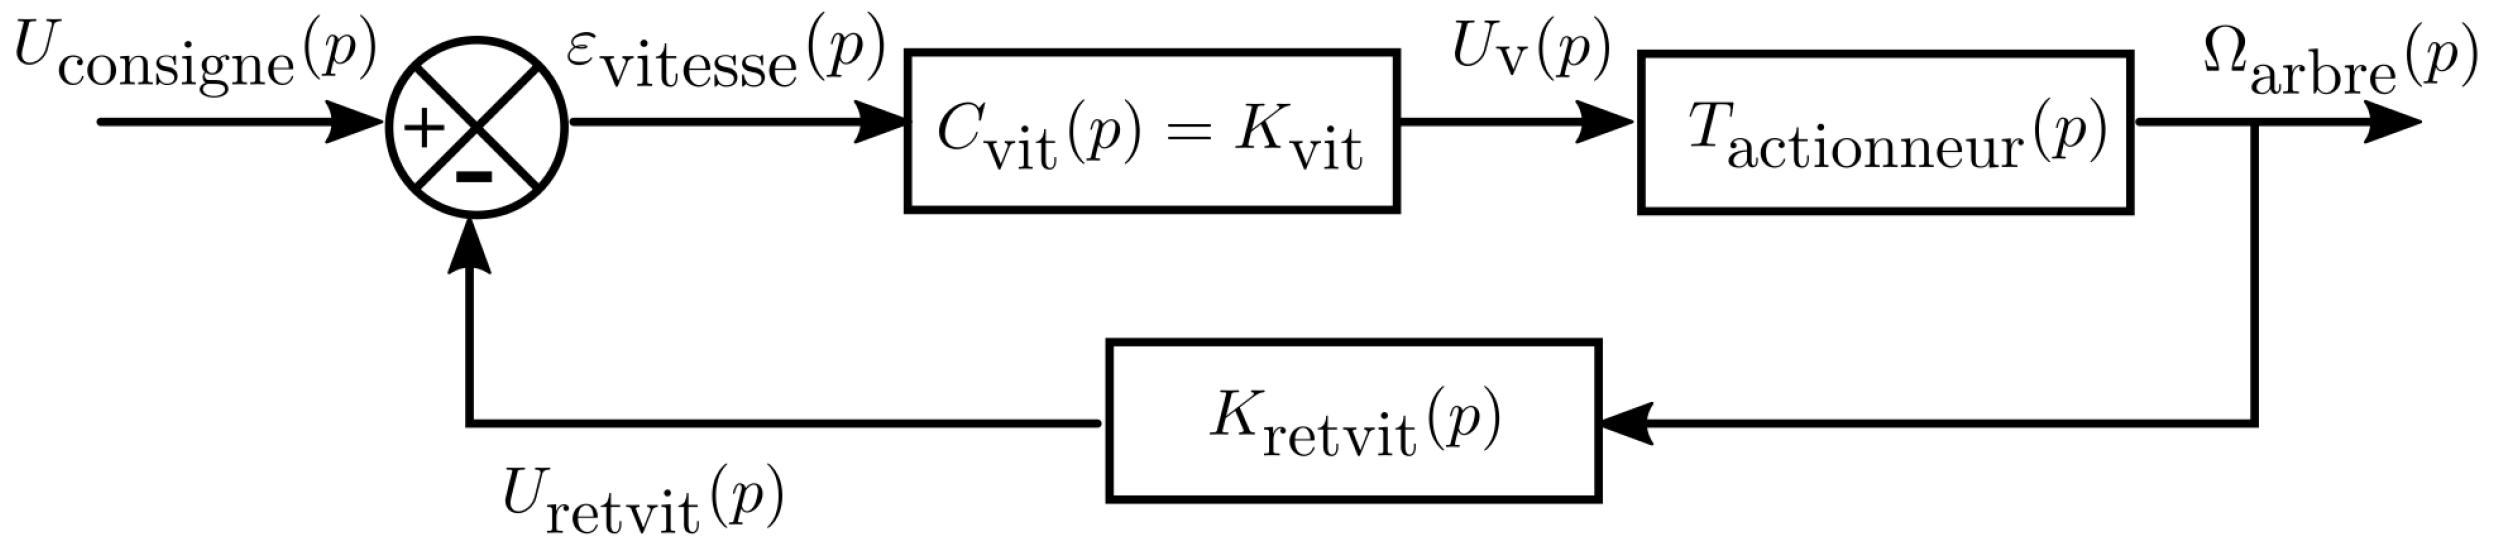
\includegraphics[width=0.7\linewidth]{img/fig18}
 \caption{Schéma simplifié de la boucle de vitesse de l'arbre}
 \label{fig18}
\end{figure}

Avec :
\begin{itemize}
 \item $u_{consigne}$, tension représentative de la consigne de vitesse de l'arbre (en $V$),
 \item $u_{retvit}$, tension représentative de la vitesse mesurée de l'arbre (en $V$),
 \item $u_v$, tension de commande du convertisseur (en $V$),
 \item $\omega_{arbre}$, vitesse de rotation de l'arbre en ($rad.s^{-1}$),
 \item $C_{vit}(p)$, fonction de transfert du correcteur à action proportionnelle,
 \item $T_{actionneur}(p)$, fonction de transfert du moteur associé à son convertisseur,
 \item $k_{retvit}(p)$, fonction de transfert associée au capteur de vitesse et son adaptation.
\end{itemize}

Remarque : par convention, les variables dans le domaine de Laplace sont notées avec des majuscules, alors qu'elles sont notées avec des minuscules dans le domaine temporel.

Un modèle obtenu à partir de l'étude fréquentielle du moteur associé à son convertisseur a permis de tracer le diagramme de Bode de la fonction de transfert $T_{actionneur}(p)=\frac{\Omega_{arbre}(p)}{U_v(p)}$. Ce diagramme de Bode est représenté sur la figure \ref{fig19}. Les asymptotes du diagramme de Bode sont représentées en pointillés.

\begin{figure}[!h]
 \centering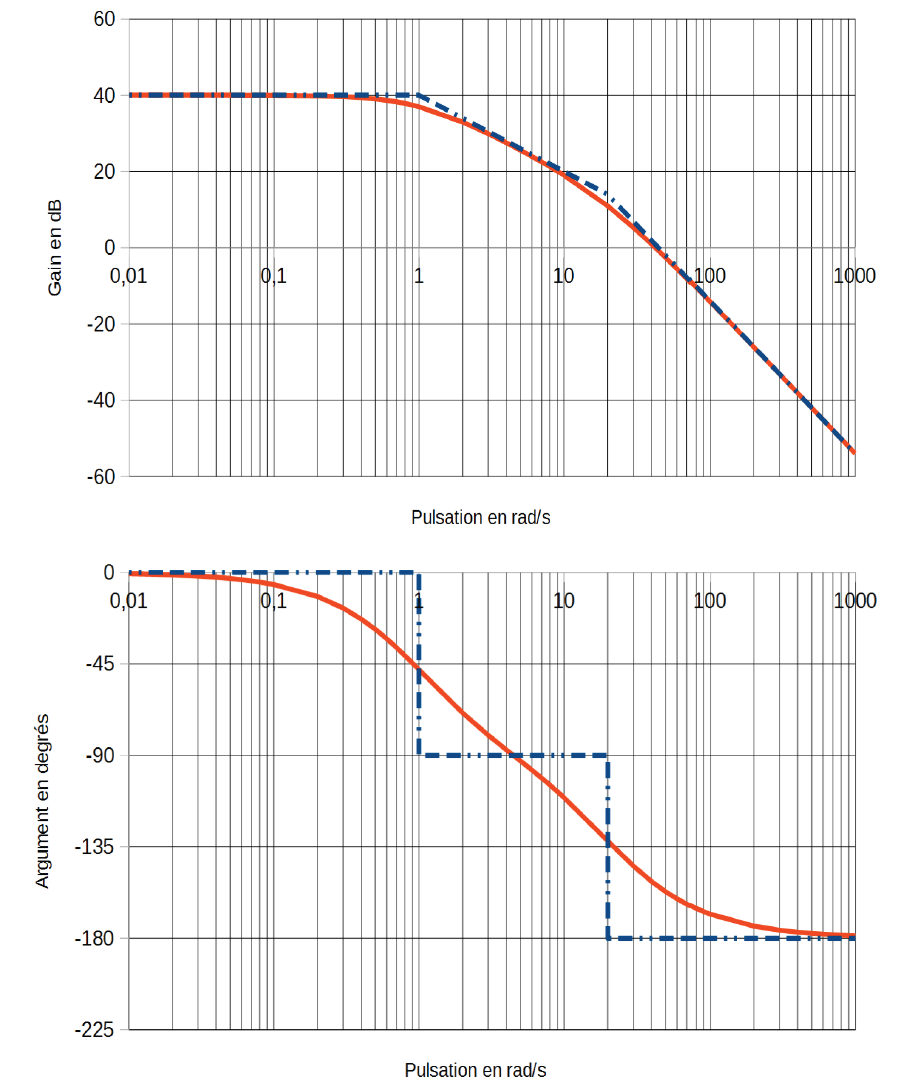
\includegraphics[width=0.7\linewidth]{img/fig19}
 \caption{Diagramme de Bode de $T_{actionneur}(p)$}
 \label{fig19}
\end{figure}

\question{À partir de l'étude de ces deux diagrammes, exprimer $T_{actionneur}(p)$ sous la forme $T_{actionneur}(p)=\frac{K_{ac}}{\left(1+\frac{p}{\omega_1}\right)\left(1+\frac{p}{\omega_2}\right)}$. Préciser les valeurs de $K_{ac}$, $\omega_1$ et $\omega_2$.}

Le capteur de vitesse délivre une tension uretvit proportionnelle à la vitesse de rotation de l'arbre.
La caractéristique de transfert de cet ensemble est donnée figure \ref{fig20}:

\begin{figure}[!h]
 \centering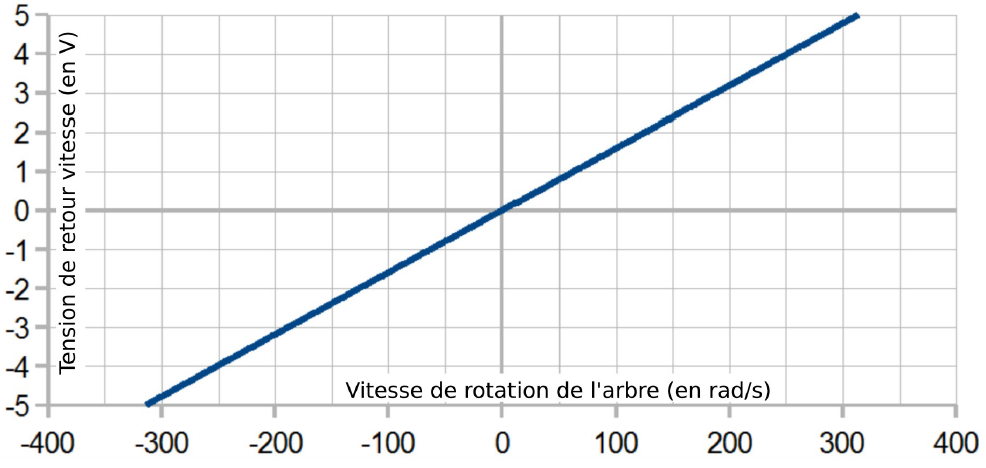
\includegraphics[width=0.7\linewidth]{img/fig20}
 \caption{Caractéristique de transfert du capteur de vitesse}
 \label{fig20}
\end{figure}

\question{Déterminer, à partir de la caractéristique donnée sur la figure \ref{fig20}, le coefficient d'amplification de la fonction de transfert $K_{retvit}(p)=\frac{U_{retvit}(p)}{\Omega_{arbre}(p)}$.}

\question{Déterminer l'expression littérale de la fonction de transfert en boucle ouverte $FTBO_{vitesse}(p)=\frac{U_{retvit}(p)}{\epsilon_{vitesse}(p)}$ en conservant dans cette expression la grandeur $K_{vit}$ du correcteur à action proportionnelle.}

\question{Tracer sur le diagramme de Bode de cette fonction de transfert en boucle ouverte pour $K_{vit}=1$.}

%\question{On souhaite régler le correcteur à action proportionnelle pour obtenir une marge de phase de 45°. Quelle valeur faut-il donner à $K_{vit}$ pour obtenir cette marge de phase ?}

\paragraph{Optimisation du temps de réponse à 5\%}
On souhaite optimiser le temps de réponse à 5\% de la boucle de vitesse. Cette optimisation risque de modifier la valeur du correcteur calculée précédemment.

L'objectif de cette partie est de calculer la valeur de $K_{vit}$ qui optimise le temps de réponse à 5\% de la boucle de vitesse et de vérifier que cette nouvelle valeur est compatible avec l'exigence de stabilité concernant la marge de phase.

\question{Exprimer la fonction de transfert en boucle fermée de la boucle de vitesse,
$FTBF_{vitesse}(p)=\frac{\Omega_{arbre}(p)}{U_{consigne}(p)}$ sous forme canonique $FTBF_{vitesse}(p)=\frac{A}{1+\frac{2\cdot m}{\omega_0}\cdot p + \left(\frac{p}{\omega_0}\right)^2}$. Préciser les expressions littérales de $A$, $\omega_0$ et $m$.}

%\question{À l'aide de la figure \ref{fig21}, déterminer la valeur à donner au coefficient d'amortissement $m$ pour optimiser le temps de réponse à 5\% de la boucle de vitesse. En déduire la valeur que l'on appellera $K_{opt}$ à donner à $K_{vit}$ permettant d'obtenir cette optimisation.}
%
%\begin{figure}[!h]
% \centering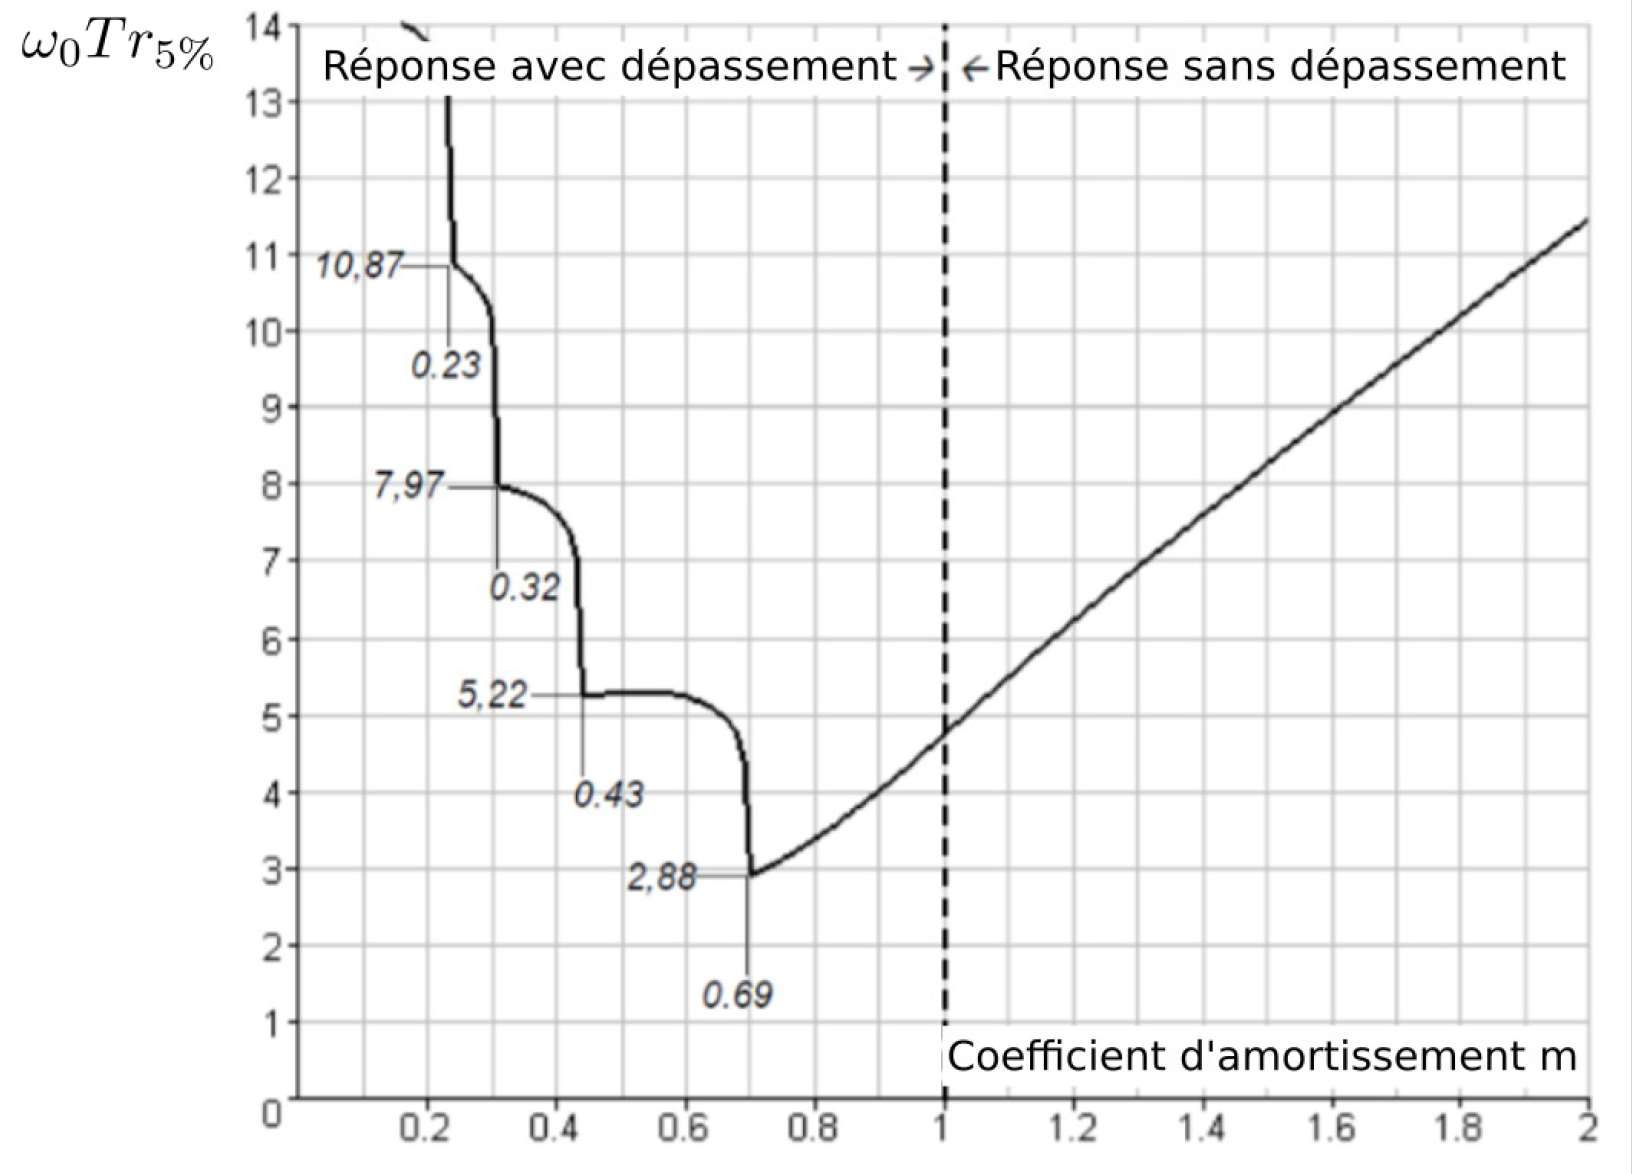
\includegraphics[width=0.7\linewidth]{img/fig21}
% \caption{Abaque du temps de réponse à 5\% réduit en fonction de $m$}
% \label{fig21}
%\end{figure}
%
%\question{Quelle est la marge de phase obtenue avec ce réglage du correcteur à la valeur $K_{opt}$ ?}
%
%\question{Conclure au regard de l'exigence de stabilité.}

\subsection{Étude de la boucle de position}

Le concepteur a choisi de contrôler indirectement l'altitude de la plate-forme d'ascenseur d'orchestre en contrôlant la position de l'arbre d'entraînement par le biais d'une boucle de position.

L'objectif de cette étude est de vérifier que l'erreur d'altitude de l'ascenseur d'orchestre sera nulle suite à un échelon appliqué à la consigne de positionnement.

Le schéma simplifié de la boucle de position de l'arbre a été remplacé par un schéma équivalent faisant apparaître une boucle de position à retour unitaire. Ce schéma équivalent est donné figure \ref{fig22}. L'altitude de l'ascenseur d'orchestre est reliée à la position de l'arbre par l'intermédiaire d'un réducteur à engrenages suivi d'un réducteur à chaîne, le tout entraînant la rotation de l'axe du Spiralift ND9.

\begin{figure}[!h]
 \centering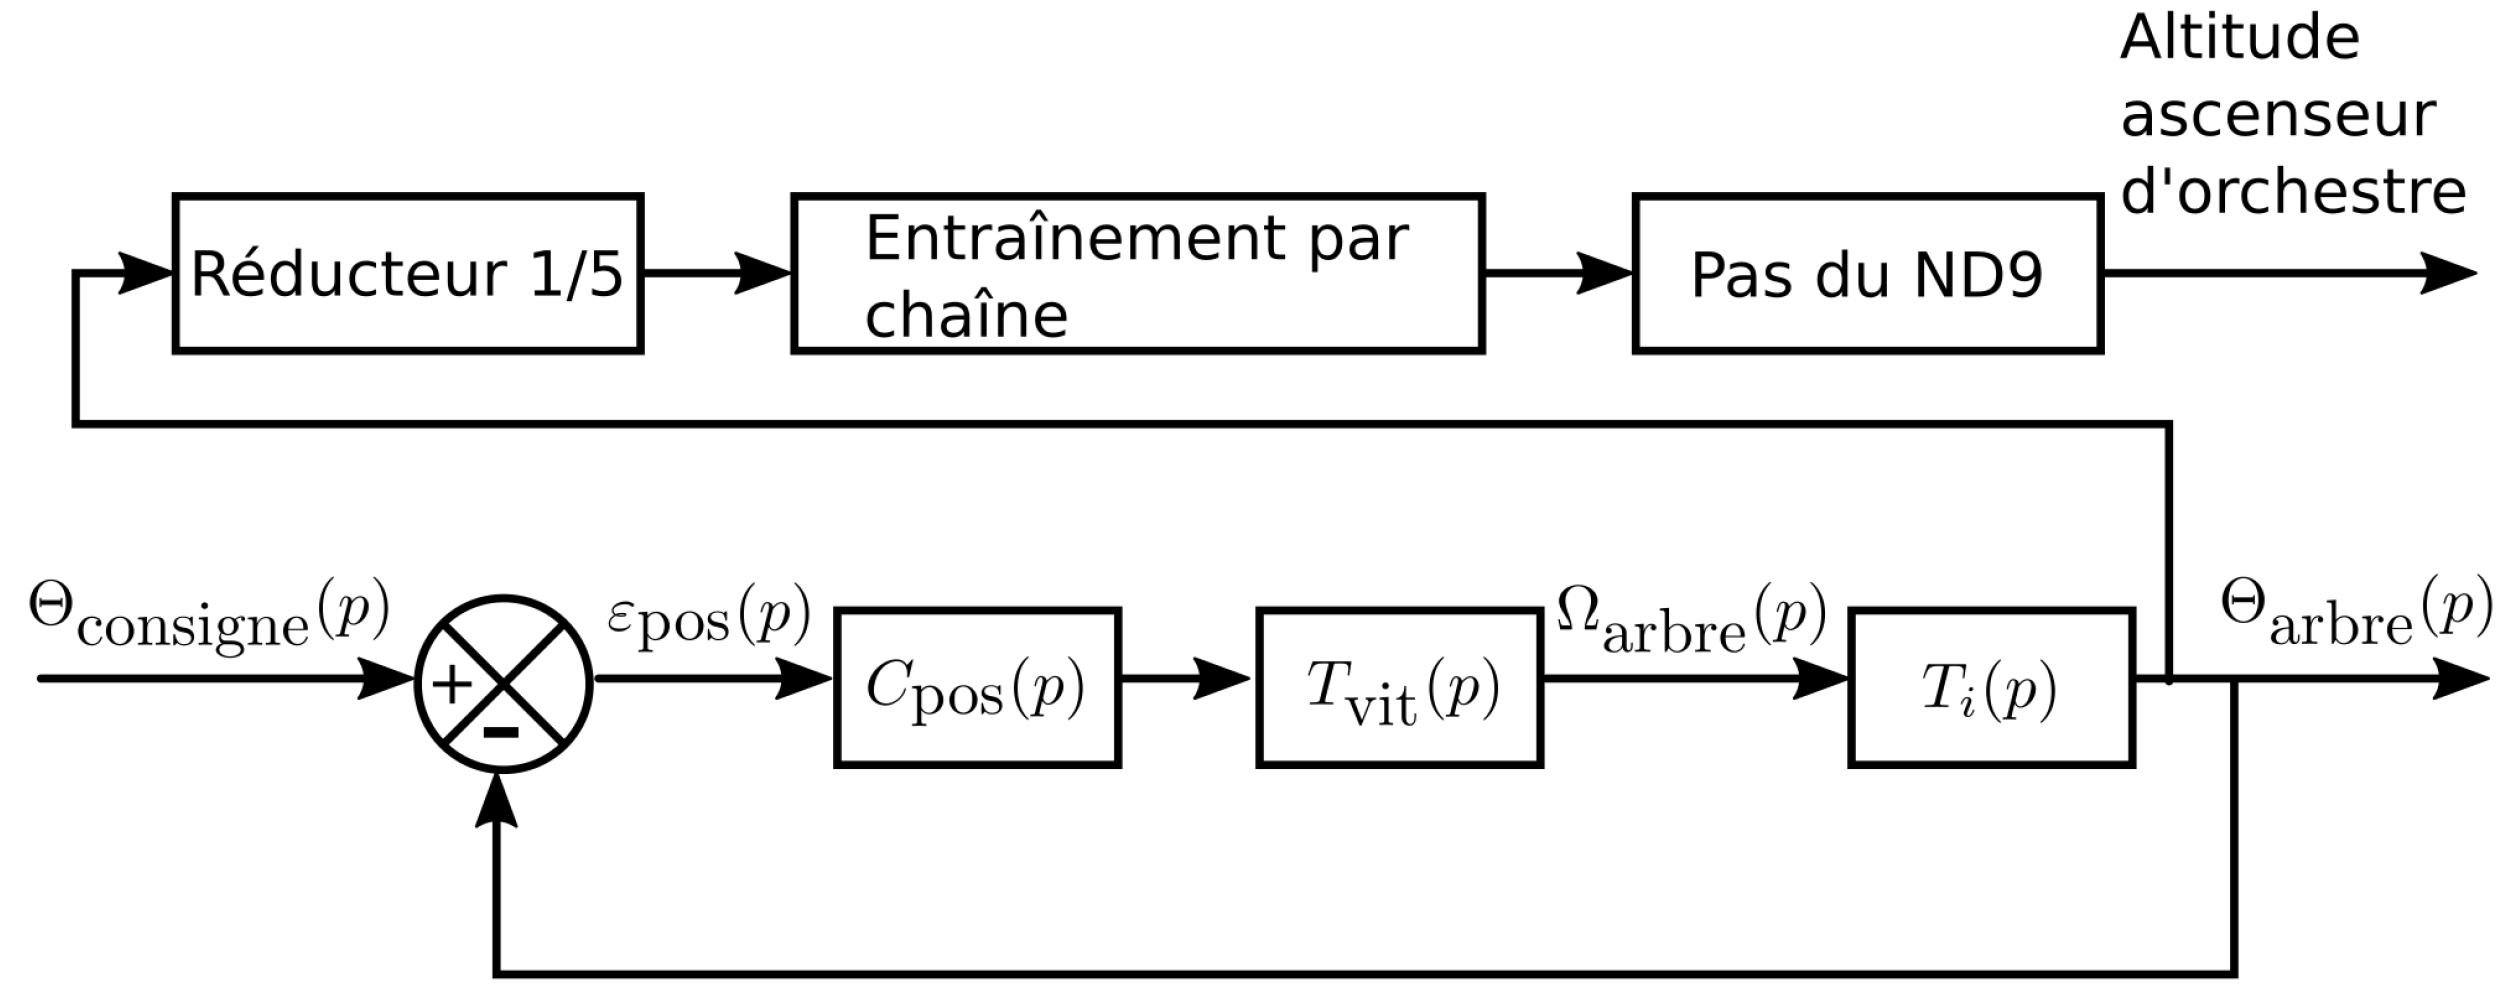
\includegraphics[width=0.7\linewidth]{img/fig22}
 \caption{Schéma simplifié de la boucle de position de l'arbre}
 \label{fig22}
\end{figure}

On note :
\begin{itemize}
 \item $\theta_{consigne}$, la grandeur représentative de la consigne de position de l'arbre,
 \item $\theta_{arbre}$, la position de l'arbre (sur plusieurs tours) (en $rad$),
 \item $\omega_{arbre}$, la vitesse de rotation de l'arbre en ($rad.s^{-1}$),
 \item $C_{pos}(p)$, la fonction de transfert du correcteur de la boucle de position,
 \item $T_{vit}(p)$, la fonction de transfert représentative de la boucle de vitesse,
 \item $T_i(p)$, la fonction de transfert permettant de passer de la vitesse angulaire à la position angulaire de l'arbre.
\end{itemize}

\question{Donner la fonction de transfert du bloc $T_i(p)=\frac{\theta_{arbre}(p)}{\Omega_{arbre}(p)}$ situé entre la vitesse de rotation de l'arbre et la position angulaire de l'arbre.}

La fonction de transfert en boucle ouverte de la boucle de position de l'arbre est donnée et vaut :
$FTBO_{posarbre}(p)=\frac{1}{p}\cdot \frac{A}{1+\frac{1,38}{\omega_0}\cdot p+\left(\frac{p}{\omega_0}\right)^2}$, où $A$ est un coefficient constant appelé coefficient d'amplification en boucle ouverte.

\question{Quelle est la classe de ce système ? En déduire l'erreur de position angulaire sur l'arbre suite à un échelon de consigne de position.}

\question{Conclure sur la satisfaction de l'exigence relative à l'erreur de position suite à un échelon de consigne.}

%\subsection{Vérification de la conformité de la résolution du capteur d'altitude}
%
%La mesure de l'altitude de l'ascenseur d'orchestre est déduite de la position angulaire (sur plusieurs tours) de l'arbre d'entraînement du Spiralift.
%
%La position angulaire de cet arbre est mesurée à l'aide d'un codeur incrémental délivrant 32 impulsions par tour, associé à un compteur. Le compteur est incrémenté de un à chaque impulsion quand la plate-forme monte (décrémenté de un à chaque impulsion quand la plate-forme descend).
%
%Le niveau le plus bas de l'ascenseur d'orchestre est détecté par un capteur de fin de course placé sur le rail de guidage.
%
%Lorsque l'ascenseur d'orchestre est à son niveau le plus bas, le compteur est mis à zéro. Ainsi, le nombre stocké au niveau du compteur est proportionnel à l'altitude de l'ascenseur d'orchestre.
%
%Données :
%\begin{itemize}
% \item la course totale de la plate-forme d'ascenseur d'orchestre est de 5,6 m,
% \item la sortie du réducteur est reliée à la couronne du Spiralift ND9 par une chaîne,
% \item le pignon associé à l'axe du réducteur, comporte 21 dents,
% \item le pignon associé à la couronne du Spiralift comporte 54 dents,
% \item Un tour de la couronne du Spiralift ND9 provoque une variation d'altitude de l'ascenseur d'orchestre d'une hauteur de 52,9 mm.
%\end{itemize}
%\begin{figure}[!h]
% \centering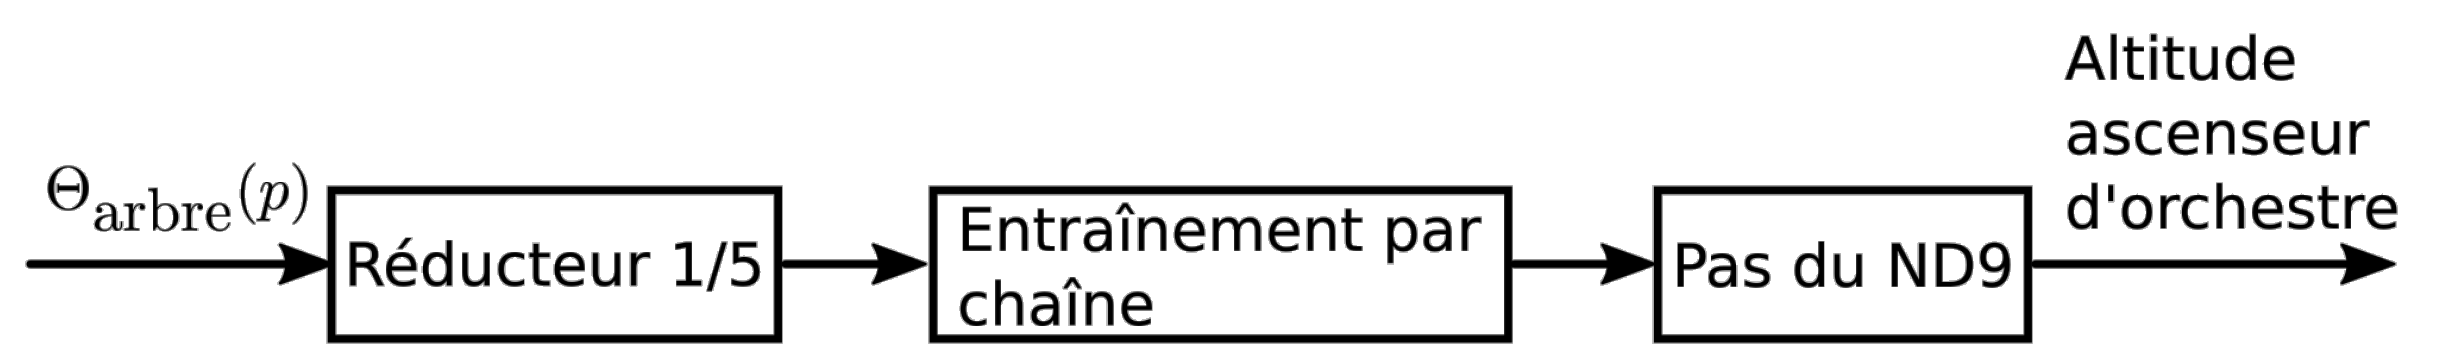
\includegraphics[width=0.7\linewidth]{img/fig23}
% \caption{Transmission à la sortie du moteur}
% \label{fig23}
%\end{figure}
%
%\question{Déterminer le plus petit écart d'altitude de l'ascenseur d'orchestre mesurable par ce dispositif et vérifier que l'exigence \og mesure de position \fg de la figure \ref{fig08} est respectée.}
%
%\question{Déterminer l'altitude du plancher de la zone de stockage par rapport à la position basse de l'ascenseur d'orchestre (voir figure \ref{fig16}) sachant que le code hexadécimal correspondant à l'altitude de ce plancher est 0x184E.}
%
%\question{Donner en binaire puis en hexadécimal le nombre codant l'altitude maximale. En déduire le nombre de bits nécessaires pour coder l'altitude de l'ascenseur d'orchestre. Ce résultat est-il conforme à l'exigence \og codage \fg de la figure \ref{fig08} ?}
%
%\question{Conclure en faisant le bilan des exigences satisfaites au niveau des asservissements.}

La pièce 4 est en réalité un assemblage entre deux pièces liées par un assemblage par vis, comme le montre la figure \ref{fig14} Cela permet de pouvoir régler la distance CD au montage du système.

\begin{figure}[!h]
 \centering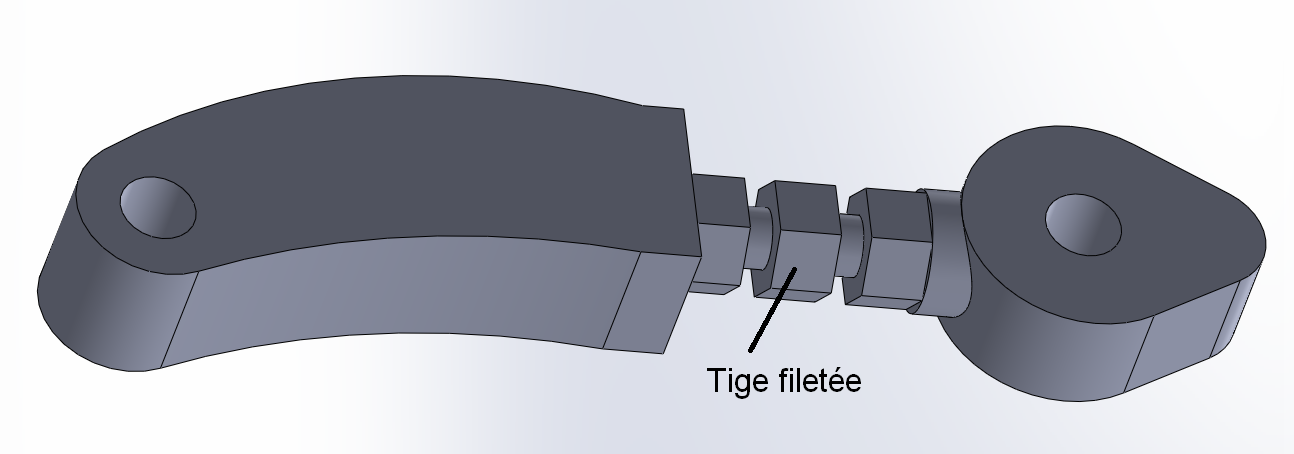
\includegraphics[width=0.7\linewidth]{img/assemblage}
 \caption{Charnière}
 \label{fig23}
\end{figure}

Afin de compenser l'hyperstatisme du système la longueur des charnières doit pouvoir être réglée. Ainsi, la charnière est un assemblage constituée de trois pièces l'une étant une tige filetée des deux côtés avec un écrou encastré au milieu, comme le montre la figure \ref{fig15}.

\begin{figure}[!h]
 \centering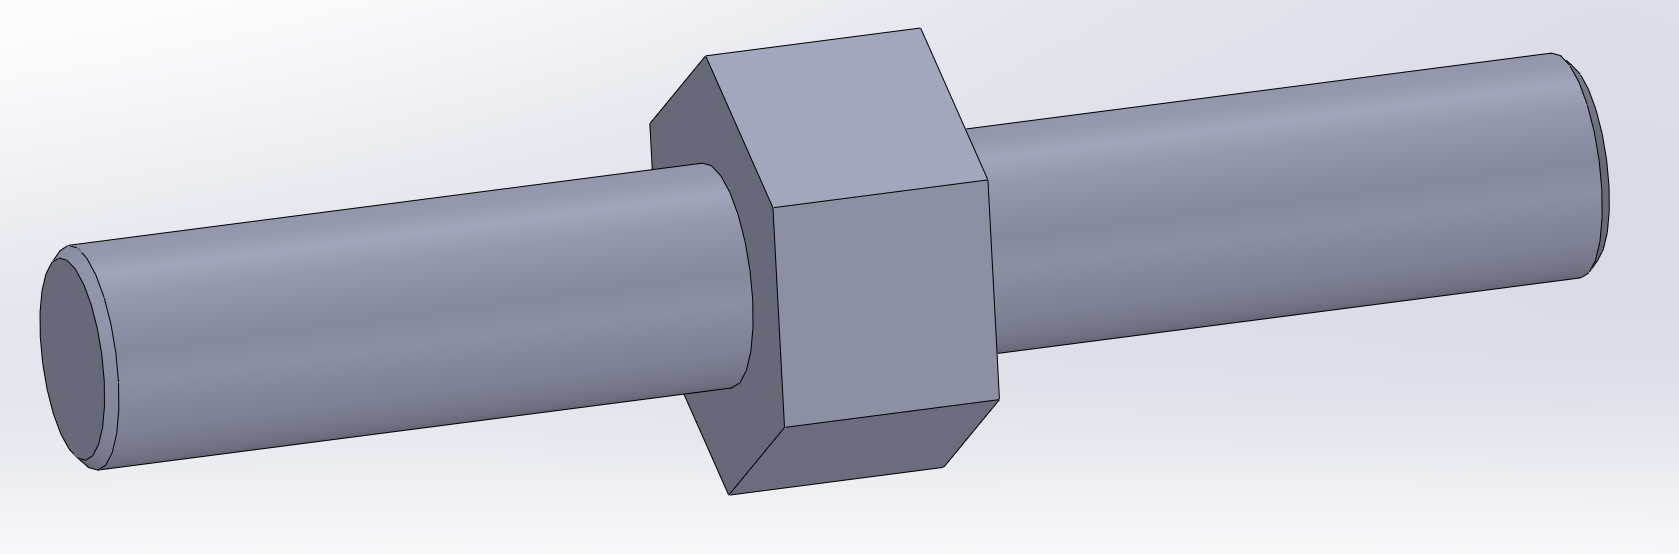
\includegraphics[width=0.6\linewidth]{img/vis}
 \caption{Tige filetée}
 \label{fig24}
\end{figure}

\question{Compléter la charnière, dans le cadre réservé à cet effet, sur la vue en coupe du document réponse.}

\question{Quelles caractéristiques doivent avoir les deux filets de chaque côté de l'écrou sur la tige filetée.}

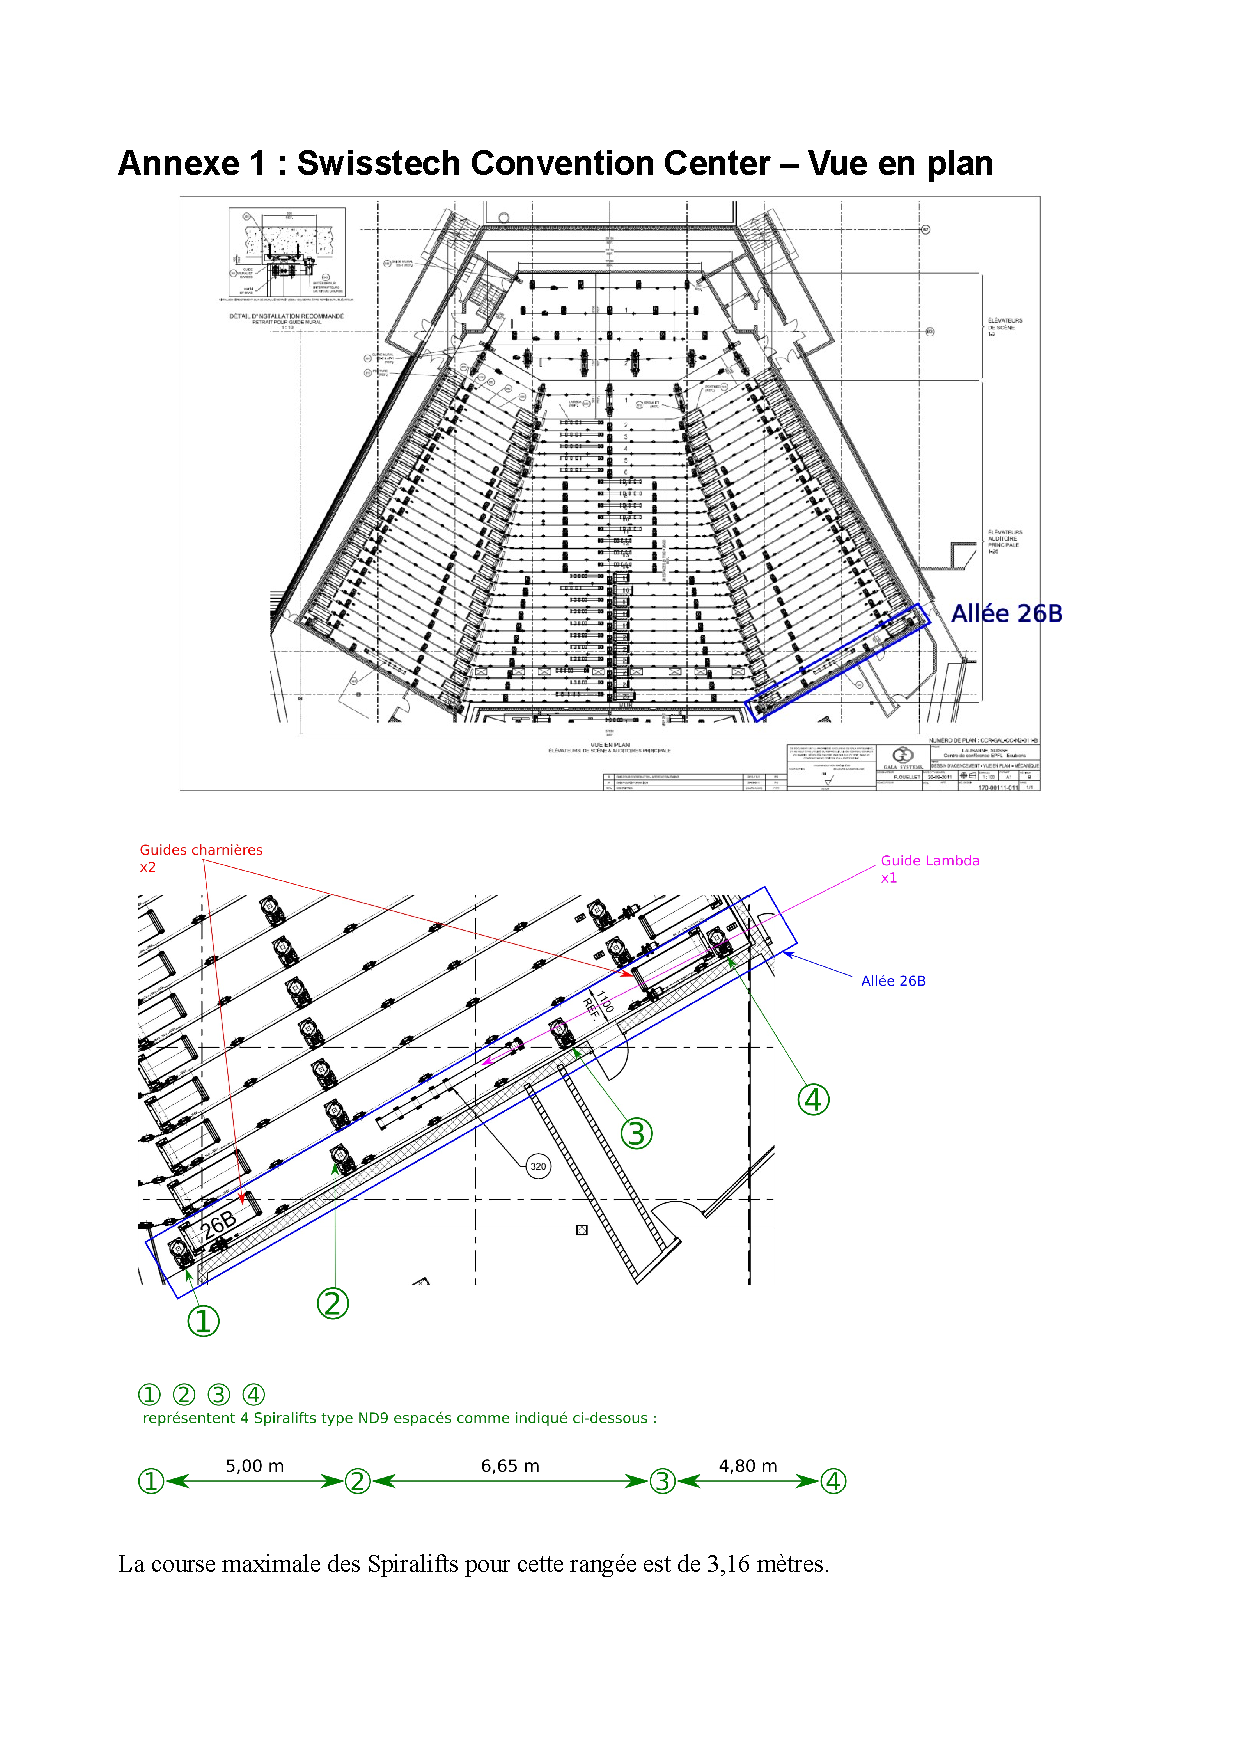
\includepdf[pages={-},scale=1,pagecommand={},offset=0cm 0cm]{img/annexes.pdf}
\newpage
\cleardoublepage

\pagestyle{documentreponse}

\section{Documents réponse}

\reponse{1}{\ifdef{\public}{
\begin{center}
\begin{tabular}{|l|l|}
\hline
$L_{0/1a}$: \hspace{5cm} & $L_{0/5}$: \hspace{5cm} \\
\hline
$L_{1a/2}$: & $L_{4/2}$:  \\
\hline
$L_{0/1b}$: & $L_{0/3}$:  \\
\hline
$L_{1b/2}$: & $L_{3/4}$:  \\
\hline
\end{tabular}
\end{center}}{
\begin{center}\begin{tabular}{|l|l|}
\hline
$L_{0/1a}$: glissière de direction $\overrightarrow{y_0}$ & $L_{0/5}$: pivot glissant d'axe $(A,\overrightarrow{z_0})$ \\
\hline
$L_{1a/2}$: ponctuelle de normale $(E_a,\overrightarrow{y_0})$ & $L_{4/2}$: sphérique de centre C \\
\hline
$L_{0/1b}$: glissière de direction $\overrightarrow{y_0}$ & $L_{0/3}$: pivot d'axe $(A,\overrightarrow{x_0})$ \\
\hline
$L_{1b/2}$: ponctuelle de normale $(E_b,\overrightarrow{y_0})$ & $L_{3/4}$: sphérique de centre B \\
\hline
\end{tabular}
\end{center}}}

\reponse{1}{\ifdef{\public}{\newpage}{\begin{center}
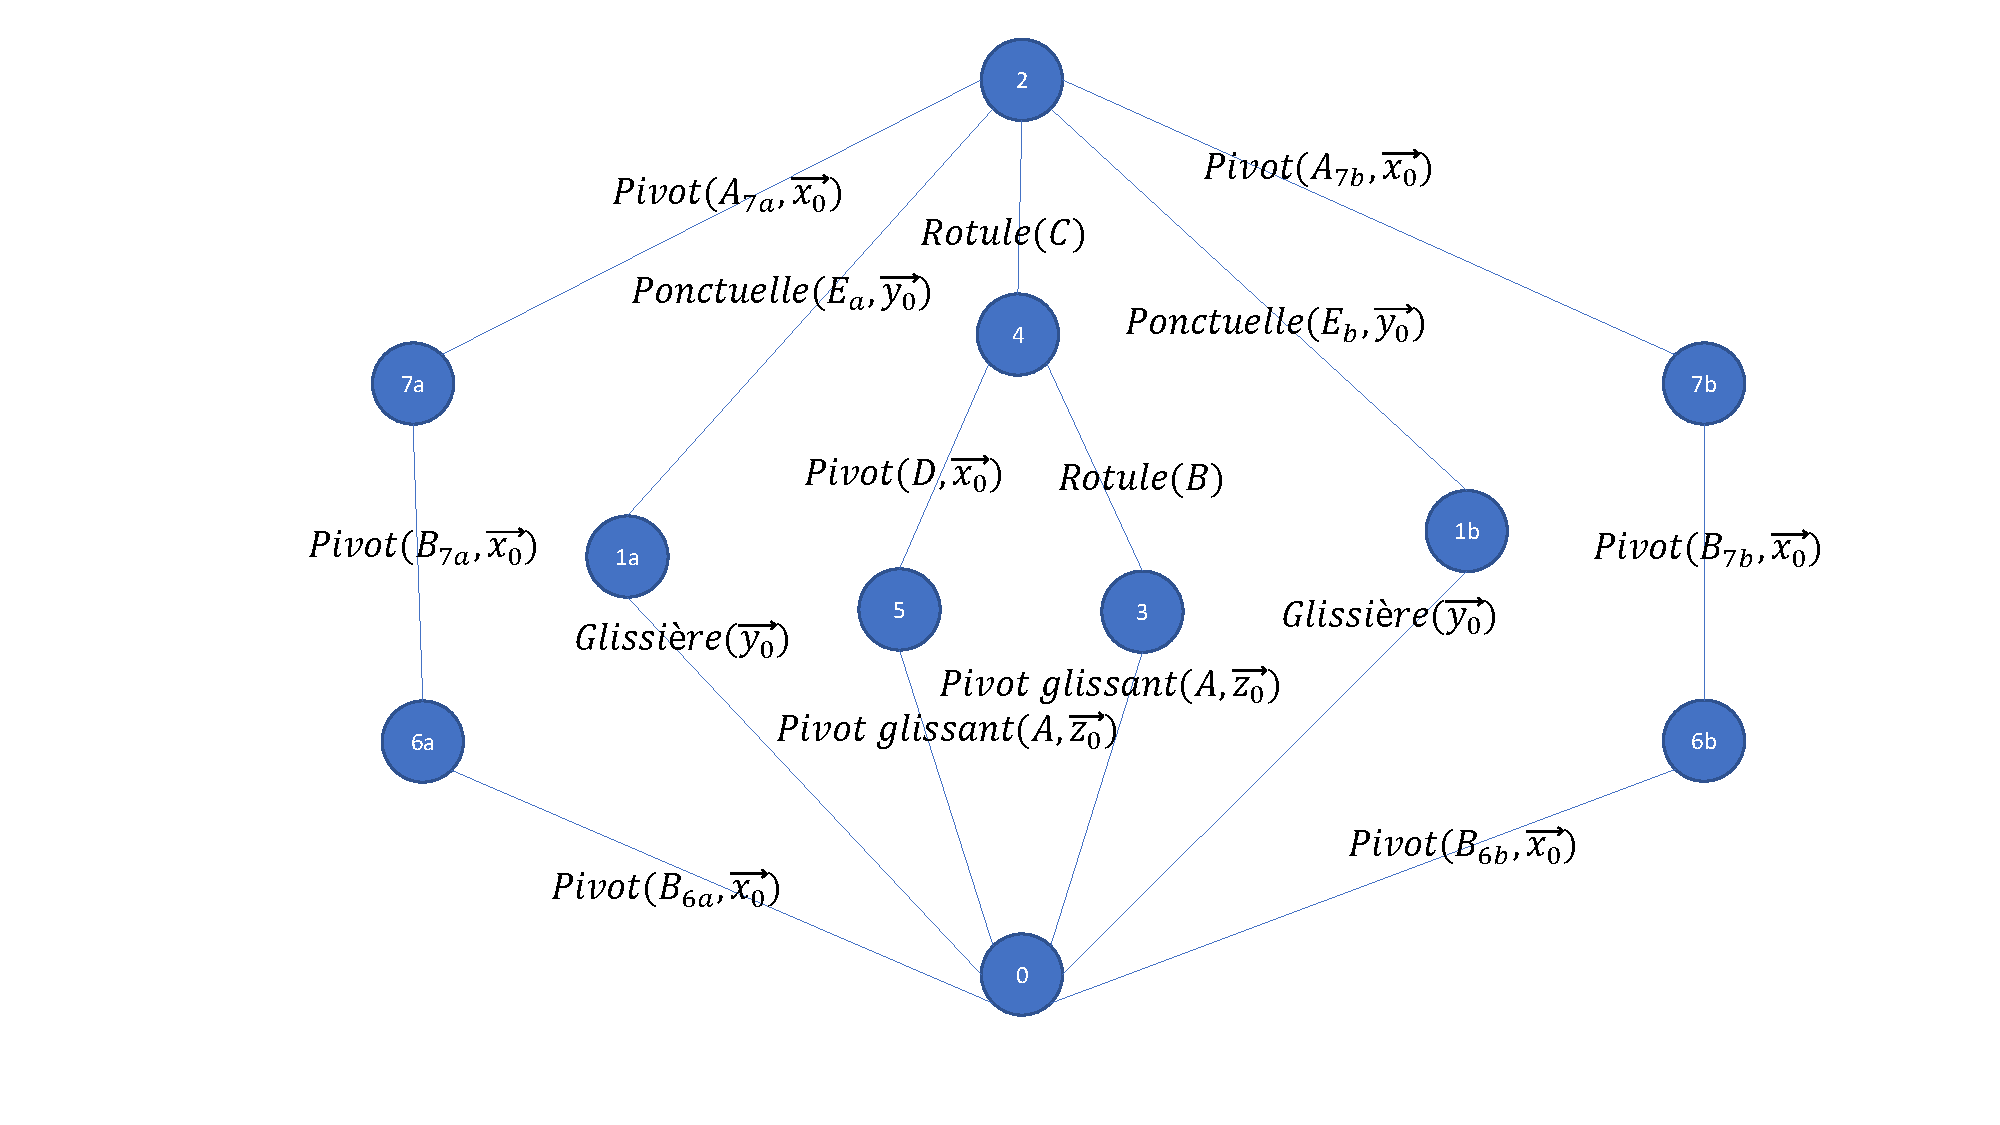
\includegraphics[width=\linewidth]{img/Graphe_liaisons}
\end{center}
\newpage}}

\reponse{1}{\ifdef{\public}{\vspace{5cm}}{$\overrightarrow{V_{C\in2/0}}=\overrightarrow{V_{C\in2/4}}+\overrightarrow{V_{C\in4/0}}=\overrightarrow{0}_{(pivot\ de\ centre\ C)}+\overrightarrow{V_{C\in4/5}}+\overrightarrow{V_{C\in5/0}}=\overrightarrow{V_{C\in4/3}}+\overrightarrow{V_{C\in3/0}}$}}

\reponse{1}{\ifdef{\public}{\vspace{5cm}}{$\overrightarrow{V_{C\in4/5}}+\overrightarrow{V_{C\in5/0}}=\overrightarrow{V_{D\in4/5}}+\overrightarrow{CD}\wedge \overrightarrow{\Omega_{4/5}}+\overrightarrow{V_{A\in5/0}}+\overrightarrow{CA}\wedge \overrightarrow{\Omega_{5/0}}=l_2.\overrightarrow{y_4}\wedge \omega_{45}\overrightarrow{x_0}+w_{50}.\overrightarrow{z_0}-l(t).\overrightarrow{y_0}\wedge \omega_{50}\overrightarrow{z_0}=-l_2.\omega_{45}\overrightarrow{z_4}+w_{50}.\overrightarrow{z_0}-l(t).\omega_{50}\overrightarrow{x_0}$\\
$\overrightarrow{V_{C\in4/3}}+\overrightarrow{V_{C\in3/0}}=\overrightarrow{CB}\wedge \overrightarrow{\Omega_{4/3}} +\overrightarrow{CA}\wedge \overrightarrow{\Omega_{3/0}}=l_1.\overrightarrow{y_4}\wedge\omega_{43}.\overrightarrow{x_0}-l(t).\overrightarrow{y_0}\wedge \omega_{30}.\overrightarrow{x_0}=-l_1.\omega_{43}.\overrightarrow{z_4}-l(t).\omega_{30}.\overrightarrow{z_0}$,

donc :
\begin{itemize}
 \item $\omega_{50}=0$,
 \item $w_{50}=-l(t).\omega_{30}$,
 \item $l_2.\omega_{45}=l_1.\omega_{43}$.
\end{itemize}}}

\reponse{1}{\ifdef{\public}{\vspace{5cm}}{$\overrightarrow{\Omega_{4/0}}=\overrightarrow{\Omega_{4/5}}+\overrightarrow{\Omega_{5/0}}=\overrightarrow{\Omega_{4/5}}+\overrightarrow{0}_{(liaison\ glissiere)}=\overrightarrow{\Omega_{4/3}}+\overrightarrow{\Omega_{3/0}}$
donc : $\omega_{45}=\omega_{43}+\omega_{30}$.}}

\reponse{1}{\ifdef{\public}{\vspace{1cm}}{Il y a 3 équations et 4 inconnues, il y a donc une seule mobilité.}}

\newpage

\reponse{1}{\ifdef{\public}{\vspace{2cm}}{A cause des charnières, le mécanisme a un mouvement plan. Il existe une rotation entre 2 et 4 autour du point C ce qui porte le nombre de mobilité à deux avec celle de la question précédente.}}

\reponse{1}{\ifdef{\public}{\vspace{2cm}}{$h=N_s-r_s$, $N_s=10*5+2*1+1*4+2*3=62$, $r_s=6.(p-1)-m=6.10-2=58$, donc $h=4$. \\
$h=6\cdot\gamma+m-I_c$, $I_c=10*1+2*5+1*2+2*3=28$, $h=6*5+2-28=4$.}}

\reponse{1}{\ifdef{\public}{\begin{tabular}{|c|c|c|c|c|}
\hline
& Guides charnières & Guide lambda & Un Spiralift seul & Combinaison de deux Spiralifts \\
\hline
$R_x=0$ & & & & \\
\hline
$R_y=0$ & & & & \\
\hline
$R_z=0$ & & & & \\
\hline
$T_x=0$ & & & & \\
\hline
$T_z=0$ & & & & \\
\hline
\end{tabular}}{\begin{tabular}{|c|c|c|c|c|}
\hline
& Guides charnières & Guide lambda & Un Spiralift seul & Combinaison de deux Spiralifts \\
\hline
$R_x=0$ & & & & X\\
\hline
$R_y=0$ & X & & & \\
\hline
$R_z=0$ & X & & & \\
\hline
$T_x=0$ & X & X & & \\
\hline
$T_z=0$ & & X & & \\
\hline
\end{tabular}}}



\reponse{1}{\ifdef{\public}{\vspace{1cm}}{$N_{moteur}=\frac{N_{max}}{r}=\frac{2,5}{1,67.10^{-3}}\approx 1497tr.min^{-1}$}}

\reponse{1}{\ifdef{\public}{%\begin{figure}[!h]
\begin{center}
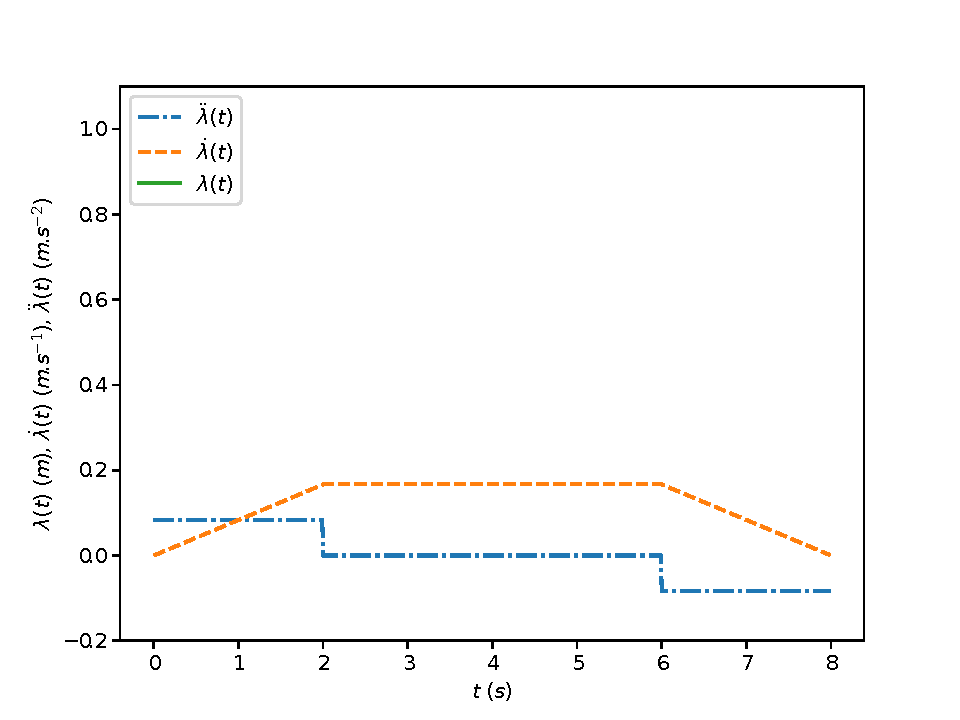
\includegraphics[width=0.7\linewidth]{img/DR14}
\end{center}
% \caption{Evolution de $\lambda\ (t)$, $\dot{\lambda}\ (t)$, $\ddot{\lambda}\ (t)$}
%\end{figure}
}{%\begin{figure}[!h]
\begin{center}
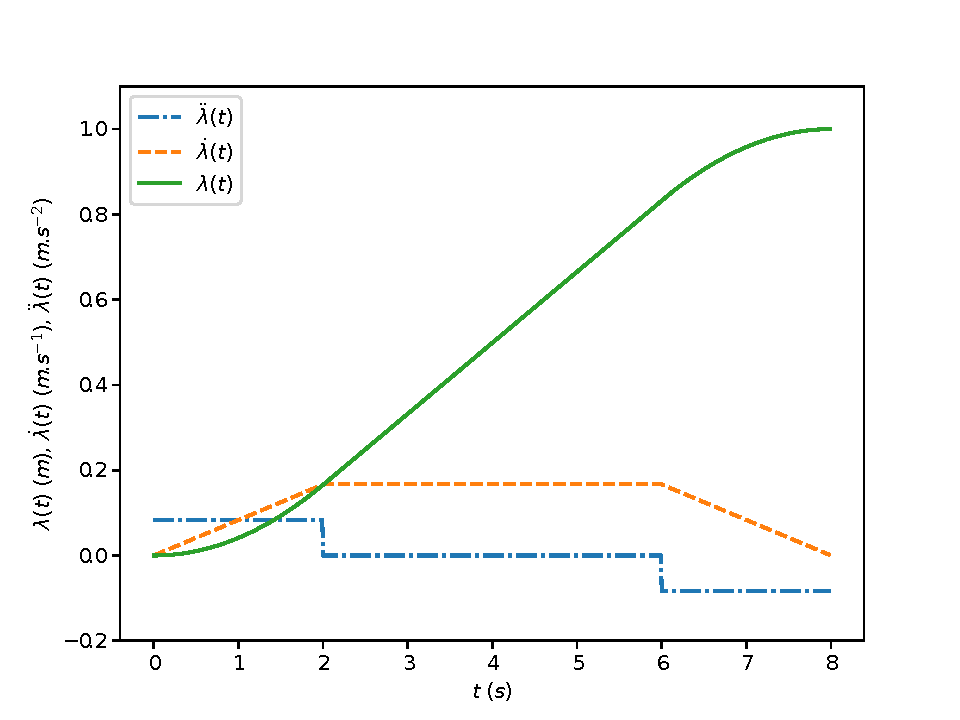
\includegraphics[width=0.7\linewidth]{img/DR14_cor}
\end{center}
% \caption{Evolution de $\lambda\ (t)$, $\dot{\lambda}\ (t)$, $\ddot{\lambda}\ (t)$. On calcule que $\lambda\ (0)=0$ $\lambda\ (8)=1$}
%\end{figure}
}}

\newpage

\reponse{1}{\ifdef{\public}{\vspace{3cm}}{Fermeture géométrique: $\overrightarrow{B_6A_7}+\overrightarrow{A_7B_7}+\overrightarrow{B_7B_6}=-l.\overrightarrow{y_6}+l.\overrightarrow{y_7}-\lambda.\overrightarrow{y_0}=-l.\left(cos\alpha_6.\overrightarrow{y_0}+sin\alpha_6.\overrightarrow{z_0}\right)+l.\left(cos\alpha_7.\overrightarrow{y_0}+sin\alpha_7.\overrightarrow{z_0}\right)-\lambda.\overrightarrow{y_0}=\overrightarrow{0}$. En projetant sur $\overrightarrow{y_0}$, on obtient $-l.cos\alpha_6+l.cos\alpha_7-\lambda=0$, donc $-l.cos(\pi-\alpha_7)+l.cos\alpha_7-\lambda=0$, d'où $\lambda=2.l.cos\alpha$.}}

\reponse{1}{\ifdef{\public}{\vspace{3cm}}{On sait que $\lambda\ (0)=0$, donc $\alpha\ (0)=\frac{\pi}{2}$ et $\lambda\ (8)=1$, donc $cos(\alpha\ (8))\neq 1$, donc $\alpha\ (8)\neq 0$, donc il s'agit de la courbe 2.}}

\reponse{1}{\ifdef{\public}{\vspace{3cm}}{$\overrightarrow{\Omega_{6/0}}=\dot{\alpha_6}.\overrightarrow{x_0}=-\dot{\alpha}.\overrightarrow{x_0}$ et $\overrightarrow{V_{B_6\in6/0}}=\overrightarrow{0}$\\
$\left\{V_{6/0}\right\}=\left\{\begin{array}{c}-\dot{\alpha}\cdot \overrightarrow{x_0} \\
\overrightarrow{0}
\end{array}\right\}_{B_6}$

$\overrightarrow{V_{G_6\in6/0}}=\overrightarrow{V_{B_6\in6/0}}+\overrightarrow{G_6B_6}\wedge \overrightarrow{\Omega_{6/0}}=\frac{l}{2}\overrightarrow{y_6}\wedge (-\dot{\alpha}.\overrightarrow{x_0})=\frac{l}{2}.\dot{\alpha}.\overrightarrow{z_6}$

$\left\{V_{6/0}\right\}=\left\{\begin{array}{c}-\dot{\alpha}\cdot \overrightarrow{x_0} \\
\frac{l}{2}.\dot{\alpha}.\overrightarrow{z_6}
\end{array}\right\}_{G_6}$}}

\newpage

\reponse{1}{\ifdef{\public}{\vspace{5cm}}{$\overrightarrow{\Omega_{7/0}}=\dot{\alpha_7}.\overrightarrow{x_0}=\dot{\alpha}.\overrightarrow{x_0}$ et $\overrightarrow{V_{B_7\in7/0}}=\dot{\lambda}\overrightarrow{y_0}$\\
$\left\{V_{7/0}\right\}=\left\{\begin{array}{c}\dot{\alpha}\cdot \overrightarrow{x_0} \\
\dot{\lambda}\overrightarrow{y_0}
\end{array}\right\}_{B_7}$

$\overrightarrow{V_{G_7\in7/0}}=\overrightarrow{V_{B_7\in7/0}}+\overrightarrow{G_7B_7}\wedge \overrightarrow{\Omega_{7/0}}=\dot{\lambda}\overrightarrow{y_0}
+\frac{l}{2}\overrightarrow{y_7}\wedge \dot{\alpha}.\overrightarrow{x_0}=\dot{\lambda}\overrightarrow{y_0}
-\frac{l}{2}.\dot{\alpha}.\overrightarrow{z_7}$

$\left\{V_{7/0}\right\}=\left\{\begin{array}{c}\dot{\alpha}\cdot \overrightarrow{x_0} \\
\dot{\lambda}\overrightarrow{y_0}-\frac{l}{2}.\dot{\alpha}.\overrightarrow{z_7}
\end{array}\right\}_{G_7}$}}

\reponse{1}{\ifdef{\public}{\vspace{4cm}}{Graphiquement, le diagramme de phase commence à 0°, puis passe par un palier à -90°, puis un dernier à -180°.

La forme proposée correspond donc avec $\omega_1=1rad.s^{-1}$ et $\omega_2=20rad.s^{-1}$, enfin, $20log(K_{ac})=40dB$, donc $K_{ac}=100rad.s^{-1}.V^{-1}$.}}

\reponse{1}{\ifdef{\public}{\vspace{4cm}}{Le coefficient $K_{retvit}$ est donné par la pente de la courbe, $K_{retvit}=\frac{4}{250}=16mV.s.rad^{-1}$.}}

\reponse{1}{\ifdef{\public}{\vspace{4cm}}{$FTBO_{vitesse}(p)=\frac{U_{retvit}(p)}{\epsilon_{vitesse}(p)}=K_{vit}\cdot T_{actionneur}\cdot K_{retvit}=\frac{K_{ac}\cdot K_{vit} \cdot K_{retvit}}{\left(1+\frac{p}{\omega_1}\right)\cdot \left(1+\frac{p}{\omega_2}\right)}$.}}

\newpage

\reponse{1}{\ifdef{\public}{\begin{center}
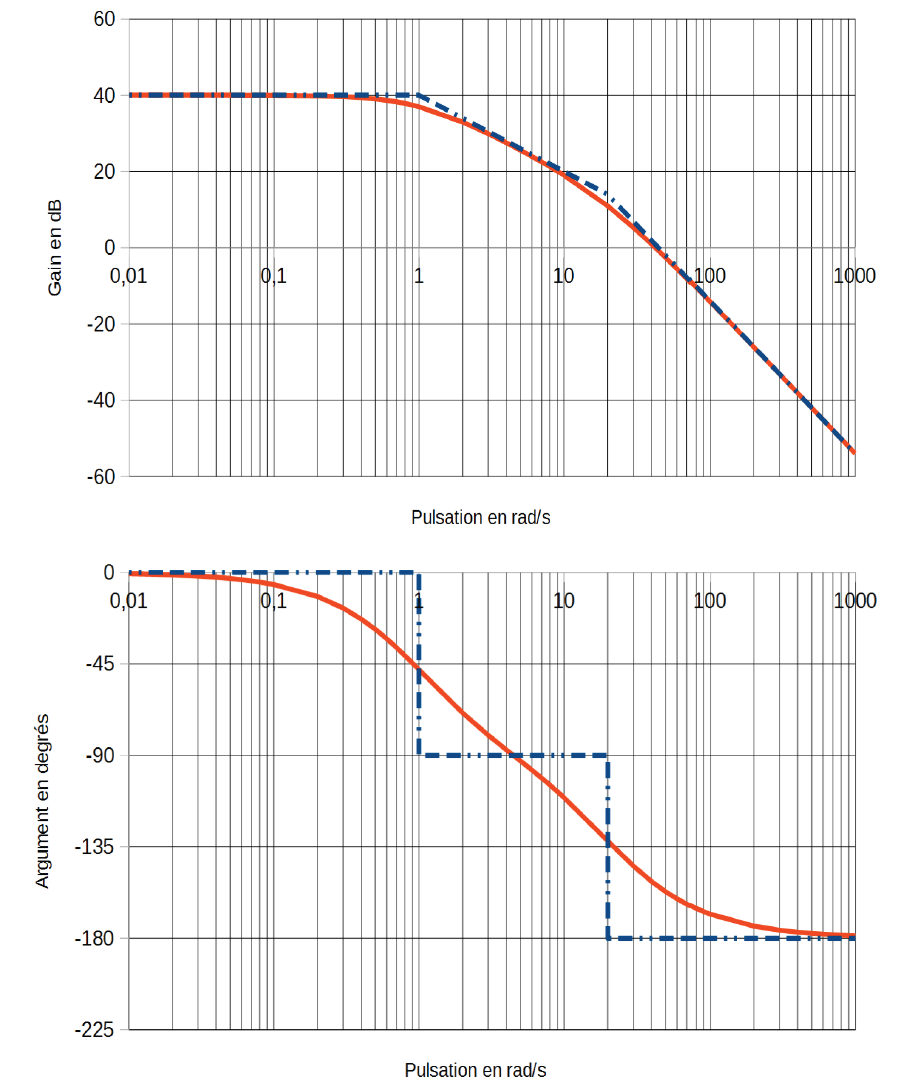
\includegraphics[width=0.7\linewidth]{img/fig19}
\end{center}}{\begin{center}
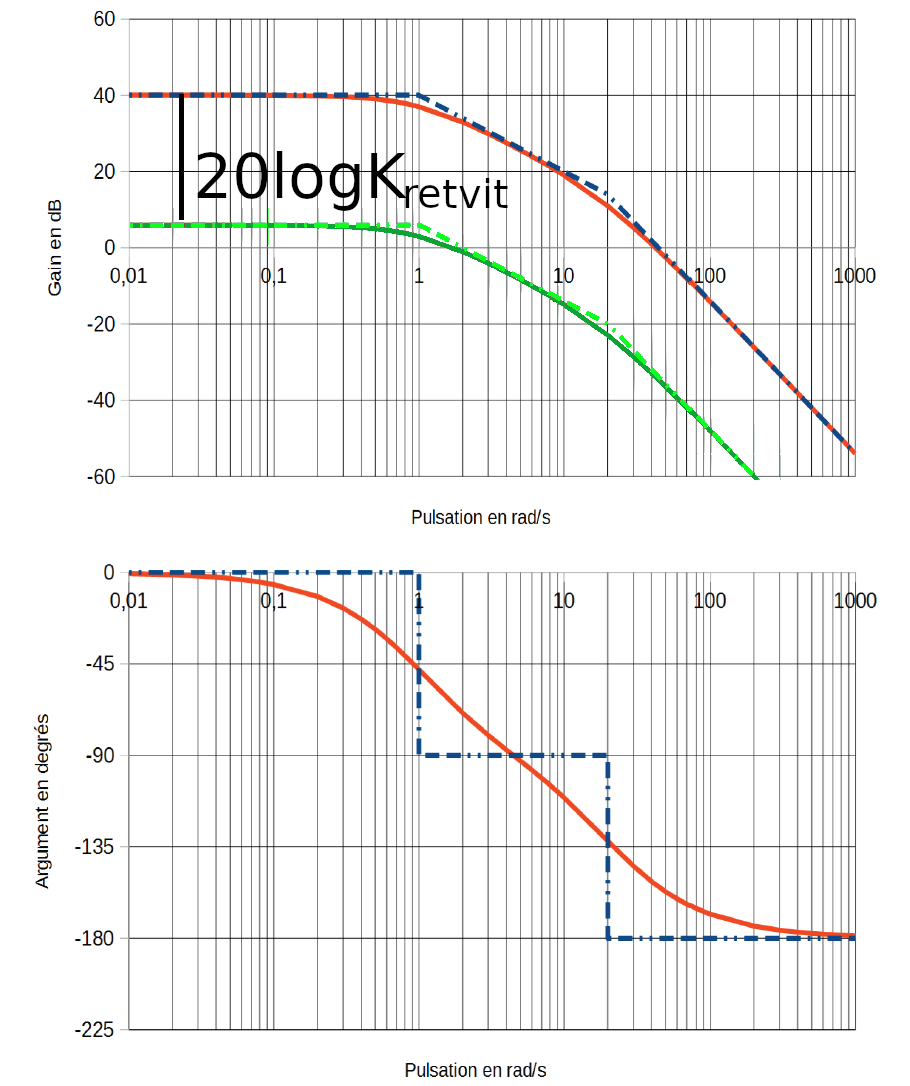
\includegraphics[width=0.7\linewidth]{img/fig19_cor}
\end{center}}}

\reponse{1}{\ifdef{\public}{\vspace{4cm}}{$FTBF_{vitesse}(p)=\frac{\Omega_{arbre}(p)}{U_{consigne}(p)}=\frac{K_{vit}\cdot T_{actionneur}}{1+K_{vit}\cdot T_{actionneur}\cdot K_{retvit}}=\frac{K_{vit}\cdot K_{ac}}{1+\left(\frac{1}{\omega_1}+\frac{1}{\omega_2}\right)\cdot p+\frac{p^2}{\omega_1\cdot\omega_2}+K_{vit}\cdot K_{ac}\cdot K_{retvit}}$

$FTBF_{vitesse}(p)=\frac{\frac{K_{vit}\cdot K_{ac}}{1+K_{vit}\cdot K_{ac}\cdot K_{retvit}}}{1+\frac{1}{1+K_{vit}\cdot K_{ac}\cdot K_{retvit}}\cdot\left(\frac{1}{\omega_1}+\frac{1}{\omega_2}\right)\cdot p+\frac{1}{1+K_{vit}\cdot K_{ac}\cdot K_{retvit}}\cdot\frac{p^2}{\omega_1\cdot\omega_2}}$.

Donc, \\
$A=\frac{K_{vit}\cdot K_{ac}}{1+K_{vit}\cdot K_{ac}\cdot K_{retvit}}$,\\
$\omega_0=\sqrt{\left(1+K_{vit}\cdot K_{ac}\cdot K_{retvit}\right)\cdot\omega_1\cdot\omega_2}$ \\
et $\frac{2\cdot m}{\omega_0}=\frac{\omega_1+\omega_2}{\omega_0^2}$,\\
donc $m=\frac{\omega_1+\omega_2}{2.\cdot \sqrt{\left(1+K_{vit}\cdot K_{ac}\cdot K_{retvit}\right)\cdot\omega_1\cdot\omega_2}}$}}


\newpage

\reponse{1}{\ifdef{\public}{\vspace{4cm}}{$T_i(p)=\frac{\theta_{arbre}(p)}{\Omega_{arbre}(p)}=\frac{1}{p}$}}

\reponse{1}{\ifdef{\public}{\vspace{3cm}}{La fonction de transfert $FTBO_{posarbre}(p)$ est de classe 1, l'erreur angulaire pour un échelon de position sera alors nulle.}}

\reponse{1}{\ifdef{\public}{\vspace{3cm}}{L'exigence est alors respectée.}}

\newpage

\reponse{1}{\ifdef{\public}{\begin{figure}[!h]
 \centering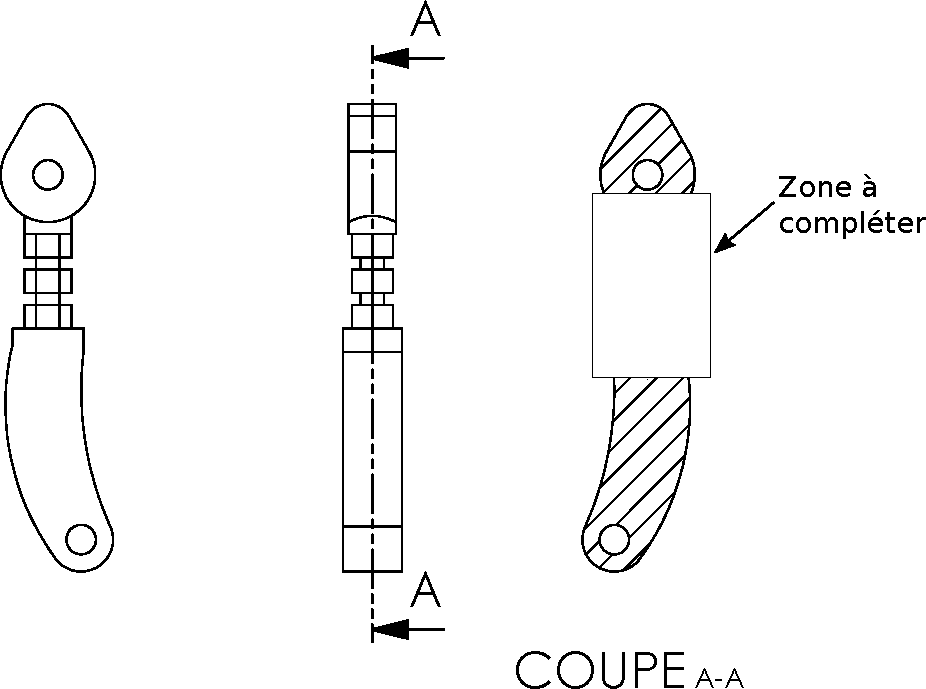
\includegraphics[width=0.7\linewidth]{img/Piece}
\end{figure}}{\begin{figure}[!h]
 \centering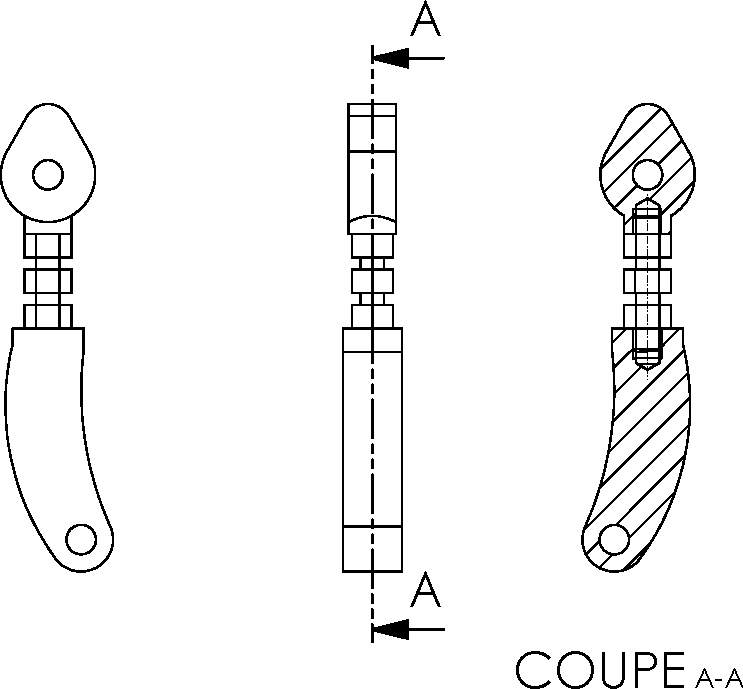
\includegraphics[width=0.7\linewidth]{img/Piece_cor}
\end{figure}}}


\reponse{1}{\ifdef{\public}{\vspace{3cm}}{Le pas de chacune des vis doit être inversé (un à droite et un à gauche).}}
\end{document}

